\documentclass{article}

\usepackage{ctex}
\usepackage{tikz}
\usetikzlibrary{cd}
%tikzit
\usepackage{tikzit}
\input{common.tikzstyles}

\usepackage[linesnumbered,ruled,vlined]{algorithm2e}

%冲突nthm
%\usepackage{amsthm}
\usepackage{amsmath}
\usepackage{amssymb}
\usepackage{mathtools} %for :=
\usepackage{stmaryrd} %for double square bracket

%\usepackage{unicode-math}
%\usepackage{chngcntr}
\PassOptionsToPackage{hyphens}{url}\usepackage{hyperref} %url解决过长的问题
\hypersetup{
    colorlinks=true,
    linkcolor=blue,
    filecolor=magenta,      
    urlcolor=cyan,
    pdftitle={Overleaf Example},
    pdfpagemode=FullScreen,
    }


\usepackage[textwidth=18cm]{geometry} % 设置页宽=18

\usepackage{blindtext}
\usepackage{bm}
\parindent=0pt
\setlength{\parindent}{2em} 
\usepackage{indentfirst}

\usepackage{listings}
%\usepackage{minted}% hightlighting

\usepackage{proof} % infer

\usepackage{xcolor}
\usepackage{titlesec}
\titleformat{\section}[block]{\color{blue}\Large\bfseries\filcenter}{\thesection}{1em}{}
\titleformat{\subsection}[hang]{\color{red}\Large\bfseries}{\thesubsection}{1em}{}
%\setcounter{secnumdepth}{1} %section 序号


\usepackage[thmmarks, thref, amsmath]{ntheorem}

\theoremstyle{plain}
\newtheorem{theorem}{Theorem}

\newtheorem{lemma}[theorem]{Lemma}
\newtheorem{corollary}[theorem]{Corollary}
\newtheorem{proposition}[theorem]{Proposition}
\newtheorem{example}[theorem]{Example}
\newtheorem{definition}[theorem]{Definition}
\newtheorem{remark}[theorem]{Remark}
\newtheorem{exercise}{Exercise}[section]
\newtheorem{annotation}[theorem]{Annotation}

\usepackage{enumitem}
\newlist{pcases}{enumerate}{3}
\setlist[pcases]{label=\textit{Case \arabic*},leftmargin=*}
\setlist[pcases,2]{label=\textit{\thepcasesi.\arabic*}}

\newlist{psubcases}{enumerate}{3}
\setlist[psubcases]{label=\textit{Subcase \arabic*},leftmargin=*}
\setlist[psubcases,2]{label=\textit{\thepcasesi.\arabic*}}

\newcounter{case}
\newcounter{subcase}[case]
\theoremheaderfont{\itshape}
\theorembodyfont{\upshape}
\newtheorem{case}{Case}
\newtheorem{subcase}{Subcase}

\theoremstyle{nonumberplain}
\theoremheaderfont{\scshape}
\theorembodyfont{\upshape}
%\theoremsymbol{\newline\raggedleft\scshape Q. E. D.\par}
\theoremsymbol{\ensuremath{\square}}
\theorempostwork{\setcounter{case}{0}}
%\theorempostwork{\setcounter{subcase}{case}}
\newtheorem{proof}{Proof}

%\newtheorem{theorem}{Theorem}[section]
%\newtheorem{case}{Case}
%\newtheorem{subcase}{Case}
%\numberwithin{subcase}{case}

\newcommand*{\xfunc}[4]{{#2}\colon{#3}{#1}{#4}}
\newcommand*{\func}[3]{\xfunc{\to}{#1}{#2}{#3}}

\newcommand\Set[2]{\{\,#1\mid#2\,\}} %集合
\newcommand\SET[2]{\Set{#1}{\text{#2}}} %

\newcommand{\inl}[1]{\ensuremath{\text{inl}~#1}}
\newcommand{\inr}[1]{\ensuremath{\text{inr}~#1}}
\newcommand{\fold}[1]{\ensuremath{{fold}_{#1}}}
\newcommand{\unfold}[1]{\ensuremath{{unfold}_{#1}}}
\newcommand{\lam}[2]{\ensuremath{\lambda #1\ldotp~ #2}} %lamx.y
\newcommand{\pair}[1]{\ensuremath{\left\langle#1\right\rangle}}
\newcommand{\projone}[1]{\ensuremath{#1.1}}
\newcommand{\projtwo}[1]{\ensuremath{#1.2}}
\newcommand{\caseof}[3]{\ensuremath{{\textbf{case}}~#1~{\textbf{of}}~\inl{x_1}\mapsto #2\mid\inr{x_2}\mapsto #3}}
\newcommand{\Lam}[2]{\ensuremath{\Lambda #1\ldotp #2}}
\newcommand{\pack}[3]{\ensuremath{{pack}~\pair{#1,#2}~{as}~#3}}
\newcommand{\unpack}[4]{\ensuremath{{unpack}~#1~{as}~\pair{#2,#3}~{in}~#4}}
\newcommand{\assign}[2]{\ensuremath{#1~\coloneqq~#2}}
\newcommand{\singletype}[1]{\text{#1}}
\newcommand{\termtype}[2]{\ensuremath{#1:#2}}
\newcommand{\type}[3]{\ensuremath{ \left\{#1:#2\relmiddle|#3 \right\}}}
\newcommand{\matgen}[2]{\ensuremath{\mu #1\ldotp#2}} %ux.y
\newcommand{\mat}[0]{\matgen{\alpha}{\tau}} %ua.t
\newcommand{\fatgen}[2]{\ensuremath{\forall #1\ldotp#2}}
\newcommand{\fat}[0]{\fatgen{\alpha}{\tau}}
\newcommand{\eatgen}[2]{\ensuremath{\exists #1\ldotp#2}}
\newcommand{\eat}[0]{\eatgen{\alpha}{\tau}}
\newcommand{\fatgent}[2]{\ensuremath{\trgb{\forall} #1\ldotp#2}}
\newcommand{\fatt}[0]{\fatgent{\alpt}{\tat}}
\newcommand{\eatgent}[2]{\ensuremath{\trgb{\exists} #1\ldotp#2}}
\newcommand{\eatt}[0]{\eatgent{\alpt}{\tat}}

\newcommand{\fail}[0]{\mi{fail}}

\newcommand{\bnfdef}[0]{\ensuremath{\mathrel{::=}}} %::=
\newcommand{\term}[1]{\ensuremath\mathsf{#1}}
\newcommand{\true}{\term{true}}
\newcommand{\false}{\term{false}}
\newcommand{\ifelse}[3]{\ensuremath{\textbf{if}~#1~\textbf{then}~#2~\textbf{else}~#3}}
\newcommand{\succt}[1]{\term{succ}~#1}
\newcommand{\pred}[1]{\term{pred}~#1}
\newcommand{\iszero}[1]{\term{iszero}~#1}
\newcommand{\seq}[2]{#1;#2}
\newcommand{\subtyp}[2]{#1<:#2}


\newcommand{\redt}[1]{\textcolor{red}{#1}}
\newcommand{\bluet}[1]{\textcolor{blue}{#1}}
\newcommand{\abracket}[1]{\ensuremath{\left< #1 \right>}}
\newcommand{\dbracket}[1]{\ensuremath{\left\llbracket\,\vcenter{\hbox{$#1$}}\,\right\rrbracket}}

%variable name
\ExplSyntaxOn 
\NewDocumentCommand{\vn}{m}
 {
   \seq_set_split:Nnn \l_tmpa_seq { ~ } { #1 }
   \int_compare:nTF { \seq_count:N \l_tmpa_seq > 1 }
    {
     \seq_set_map:NNn \l_tmpb_seq \l_tmpa_seq { \exp_not:N \mathit { ##1 } }
     (\seq_use:Nn \l_tmpb_seq { \  })
    }
    { \mathop{}\!\mathit{#1} }
 }
\ExplSyntaxOff

\begin{document}
\title{Proof Theory}
\author{枫聆}
\maketitle
\tableofcontents


\newpage
\section{Basic Logic}

\subsection{Logical Framework}

%meta logic
%object logic

\begin{definition}
\rm \redt{Meta logic} is the logic that used to formalize anthor logic
\end{definition}

\begin{definition}
\rm \redt{Object logic} is the logic that formalized from meta logic.  
\end{definition}

\begin{definition}
\rm Implementations of meta logics to represent and reason about  object logics are called \redt{logical frameworks}.
\end{definition}

\begin{annotation}
\rm 上面提到的implementations实际上就是languages,例如Prolog是这样的一个language,它以Horn clause作为meta logic. 你要实现的object logic可以通过这个language来进行encoding,也就是所谓的representating,同时还可以在encoding基础上进行reasoning.  
\end{annotation}

\newpage
\subsection{First Order Logic}

\begin{example}
\rm 给定一个statement:

"Every natural number is even or odd, but not both."

如果我们想要构造一个system去accept这个statement,我们需要说明natural number是什么? even和odd又是什么? 如何描述even和odd是冲突的? 这里引出这个system需要描述的三个重要部分: \redt{objects, their properties, and relations between them}. 同时如何描述every natural number? 这里又涉及到了quantifiter.  
\end{example}

\begin{annotation}
\rm 我遵循描述一个logical system, 首先定义里面的terms, 再描述由这些terms构成的formulas.
\end{annotation}

\begin{definition}
\rm A signature $\sigma$ consist of \emph{constant symbols}, \emph{function symbols} and \emph{predicate symbols}.  
\end{definition}

\begin{definition}
\rm Let $\sigma\text{-}terms$ be a set of terms in first order logic, it defined by the follow inductive process:
\begin{enumerate}
	\item Each variable $x \in \sigma\text{-}terms$.
	\item Each constant symbol $a \in \sigma$, then $a \in \sigma\text{-}terms$.
	\item If $t_1,\cdots,t_2 \in \sigma\text{-}terms$ and $f$ is $k$-ary function symbol in $\sigma$, then $f(t_1,\cdots,t_k)\in \sigma\text{-}terms$. 
\end{enumerate}
Let $\mathcal{F}_{\sigma\text{-}terms}$ be a set of formulas in first order logic defined by follow inductive process:
\begin{enumerate}
	\item Given terms $t_1, \cdots, t_k \in \sigma\text{-}terms$ and $k$-ary predicate symbol $P$ then $P(t_1,\cdots,t_k)$ is a term. 
	\item All formulas relate to logical connective in propositional logic.
	\item If $F \in \mathcal{F}_{\sigma\text{-}terms}$ and $x$ is a variable, then $\forall x. F$ and $\exists x. F$ are both in $\mathcal{F}_{\sigma\text{-}terms}$. 
\end{enumerate}
\end{definition}

\begin{annotation}
\rm 在理解propositional logic的基础上,只要记住几个关键词\emph{function}, \emph{predicate}, and \emph{quantifier}就足以刻画first order logic. 
\end{annotation}

\begin{definition}
\rm An \redt{atomic formula} or \redt{atom} in first-order logic is simply a predicate applied to a tuple of terms; that is, an atomic formula is a formula of the form $P (t_1,\cdots,t_n)$ for $P$ a predicate, and the $t_i$ terms.
\end{definition}

\begin{annotation}
\rm 上面first-order logic里面atoms的定义可以好好想想. 我们可能之前印象中atoms只有constants symbols,现在多了一个predicates. 
\end{annotation}

\begin{definition}
\rm An atomic formula is a \redt{literal}. and if $a$ is an atomic formula, then $\neg A$ is a literal.
\end{definition}

\begin{definition}
\rm A finite set (possibly empty) of literals and logical connectives is called a \redt{clause}. The \redt{empty clause} is denoted by $\square$.
\end{definition}

\begin{annotation}
\rm \bluet{一个clause用什么connective取决于context}. 注意在connective为disjunction下的empty clause的真值可以总是被解释为false,这是因为当你考虑clause $\square \vee C$的时候,其中$C$是一个任意的clause,那么$\square \vee C$的真值实际上就是$C$的真值,这正好对应了monoid $(\{true,false\}, \vee)$,在它里面$false$ is the neutral element, 所谓neutral element就是说对这个monoid里面任意一个元素$a$都有$false ~\vee a = a$. 当connective为conjunction的时候,此时empty clause的真值总是可以被解释为true,同理. 
\end{annotation}

\begin{definition}
\rm A literal which contains no variables os called a \redt{ground literal}.
\end{definition}

\begin{definition}
\rm A clause, each member of which is a \redt{ground literal}, is called a ground clause. In particular $\square$ is ground clause.
\end{definition}

\newpage
\subsection{Logical Formulas Means}

\begin{definition}
\rm An \redt{interpretation} of a logic formula $F$ is the assignment of meanings to the symbols of $F$.
\end{definition}


\begin{definition}
\rm If $F$ is true under an interpretation $\mathcal{I}$, then $\mathcal{I}$ is called a \redt{model} of $F$
\end{definition}

\begin{annotation}\label{model-2nd-def}
\rm 关于model的另一种解释是: a set of ground literals which does not include a complementary pair $(a, \neg a)$. 
\end{annotation}

\begin{definition}
\rm A formula $F$ is \redt{satifiable} if it has a model. It is \redt{unsatisfiable} if it has no model.
\end{definition}

\begin{definition}
\rm A formula $F$ is \redt{valid} if it is true under every interpretation.
\end{definition}

\begin{theorem}\label{vaild-and-unsat}
\rm In classical logic:
\[
	F~\text{vaild} \leftrightarrow \neg F ~\text{unsatisfiable}.
\]
\end{theorem}


\newpage
\subsection{Logical Formula Transformations}

\begin{definition}
\rm A formula $F$ is in \redt{prenex normal form} if $F$ is composed by a sequence of quantifier followed by a quantifier-free part(called the matrix)
\end{definition}

\begin{example}
\rm 例如$\forall x.\forall y. F(x,y)$,其中$F$ is quantifier-free,那么这个就是一个prenex normal form.
\end{example}

\begin{definition}
\rm A formula $F$ is in \redt{negation normal form} if all its negation are applied to atoms.
\end{definition}

\begin{definition}
\rm A formula $F$ is in \redt{conjunctive normal form} (CNF) if it is a conjunction $C_1 \wedge \cdots \wedge C_n$, where $C_1 \wedge \cdots \wedge C_n$, where each $C_i$ is disjunction of literals (i.e., atoms or negated atoms). Each $C_i$ is called a \redt{clause}.
\end{definition}

\begin{definition}
\rm Let $F$ be a formula in prenex normal form. The \redt{skolemization} of $F$ consists on replacing every existentially  quantifered varible $y$ by a fresh function symbol $f(x_1,\cdots,x_n)$, where $x_1, \cdots, x_n$ are the universally quantified varaibles occurring before $y$ in the prefix of $F$. Additionally the existential quantification on $y$ is removed. When there are no more existential quantifiers left the formula is \redt{skolemized}. The $f$ is called \redt{Skolem function} (or \redt{Skolem constant} if it is of zero arity) and the term $f(x_1,\cdots,x_n)$ is called \redt{Skolem term}.
\end{definition}

\begin{example}
\rm 例如给定$\exists x. \forall y. \exists z. P(x,y,z)$,它对应的skolemization为$\forall y. P(c,x,f(y))$.
\end{example}

\begin{theorem}
\rm (\redt{Skolemization does not change sat}) The satisfiability of $F$ under skolemization is equivalent.   
\end{theorem}

\begin{proof}
\rm 考虑任意的formula $F = \forall x_1. \cdots \forall x_n. \exists y R(x_1, \cdots, x_n, y)$. 这里我们可以拆解一下model, 定义一个$M$, which contains evalutions for every function $f$ in $F$. 如果$F$ is satified under $M$ if and only if,for each possible terms for $x_1,\cdots, x_n$ (actually are strings that contains $x_i$) under the domain of functions in $M$, there exists a term for $y$ under the domain of functions in $M$ that makes $R(x_1,\cdots,x_n,y)$ is true. 因此根据axiom of choice, there exists a function $f$ such that $y = f(x_1,\cdots,x_n)$,然后我们把这个$f$再加到$M$上,这样$ \forall x_1. \cdots \forall x_n. R(x_1, \cdots, x_n, f(x_1,\cdots,x_n))$ is also satified under $M \cup f$. 
\end{proof}

\begin{annotation}
\rm Skolemization里面实际使用了second-order logical equivalence:
\[
	\forall x. \exists y. R(x,y) \iff \exists f. \forall x. R(x,f(x))
\]

\end{annotation}

\newpage
\subsection{Satisfiabitity of Logic Formulas}

\begin{annotation}
\rm 如果考虑logic formulas $F = C_1 \wedge \cdots \wedge C_n$,其中$C_i$ is clause with disjunction, 注意$F$里面的出现的variables都是被universal quantified,这是只是implicitly化了. 可以想想一旦$F$里面存在某个empty clause,那么显然$F$ is unsat, 因为empty clause is always false. 
\end{annotation}

\begin{annotation}
\rm 现在只记录一下当下我自己的思考,未来会系统补充. 
\begin{itemize}
	\item 关于connectives对sat的影响:
		\begin{itemize}
			\item 若$F = F_1 \vee F_2$ and $F$ is unsat, 那么需要$F_1$ is unsat和$F_2$ is unsat. 
			\item 若$F = F_1 \wedge F_2$ and $F$ is unsat,那么需要$F_1$ is unsat或者$F_2$ is unsat. 
		\end{itemize}
		可以看到它和connectives的关系好像是反过来了. 		 
\end{itemize}
\end{annotation}


\newpage
\subsection{Satisfiability of Sets of Formulas}

\begin{definition}
\rm If $v$ is a \redt{valuation}, this is, a mapping from the atoms to the set $\{t,f\}$.   
\end{definition}


\begin{definition}
\rm \cite{cs245-sat} Let $\Sigma$ denote a set of well-formed formulas and $t$ a valuation. Define 
$$
\Sigma^t = \left\{
\begin{aligned}
T &&& \text{if for each}~\beta \in \Sigma, \beta^t = T \\
F &&& \text{otherwise}
\end{aligned}\right.
$$
When $\Sigma^t = T$, we say that $t$ \redt{satisfies} $\Sigma$. A set $\Sigma$ is \redt{satisfiable} iff there is some valuation $t$ such that $\Sigma^t = T$. 
\end{definition}


\begin{definition}
\rm Let $\Sigma$ be a set of formulas, and let $\alpha$ be a formula, we say that 
\begin{enumerate}
	\item $\alpha$ is a \redt{logical consequence} of $\Sigma$, or
	\item $\Sigma$ \redt{(semantically) entails} $\alpha$, or
	\item $\Sigma \models \alpha$,
\end{enumerate}
if and only if for all truth valuations $t$, if $\Sigma^t = T$ then also $\alpha^t = T$. We write $\Sigma \nvDash \alpha$ for there exists a truth valuation $t$ such that $\Sigma^t = T$ and $\alpha^t = F$. 
\end{definition}

\begin{annotation}
\rm For example, $\Sigma = \{p_1,p_2,\cdots,p_n\}$ could be a set of premises and let $\alpha$ could be the conclusion that we want to derive. 
\end{annotation}

\newpage
\subsection{Classic Propositional Modal Logic}


\begin{definition}
\rm \cite{15-816-cml}Let $\Sigma$ be a set of propositional letters or atomic propositions. The set $F_P(\Sigma)$ of formulas of classical propositional modal logic is the smallest set with:
\begin{enumerate}
	\item If $A \in \Sigma$ is a propositional letter, then $A \in F_P(\Sigma)$;
	\item If $\phi,\psi \in F_P(\Sigma)$, then $\neg \phi, (\phi \wedge \psi), (\phi \vee \psi), (\phi \to \psi) \in F_P(\Sigma)$;
	\item If $\phi \in F_P(\Sigma)$, then $(\square \phi),(\Diamond \phi) \in F_P(\Sigma)$. 
\end{enumerate}
\end{definition}

\begin{definition}
\rm Let $\mathcal{S}$ be a system of modal logic, this is $F_P(\Sigma)$ with a set of axioms and rules. If axioms and rules as follow
$$
\begin{aligned}
&\text{all propostional tautologies}&(\text{P}) \\
&\square(\phi \to \psi) \to (\square\phi \to \square\psi)& (\text{Kripke axiom})\\
&\square\phi \to \phi & (\text{T}) \\
&\square\phi \to \square\square\phi &(4) \\
&\infer{\psi}{\phi & \phi \to \psi} & (\text{modus ponens})\\
&\infer{\square \phi}{\phi} & (\text{G\"{o}del}) 
\end{aligned}
$$
We call it modal logic $\mathcal{S}4$.
\end{definition}


\begin{annotation}
\rm Kriple axiom原本的形式应为
$$
\square \phi \wedge \square(\phi \to \psi) \to \square \psi
$$
上面是它经常用的等价形式. Axiom T是指若$\phi$ is necessary, 那么$\phi$ is true. Axiom 4是指$\phi$ is necessary, 那么命题"$\phi$ is necessary" is necessary, 有点别扭,举个形象的例子如果box是指某个人知道某件事,假设我知道$A~true$, 那么我肯定知道我知道$A~true$. 最后一个叫G\"{o}del translation, 它将intuitionistic logic里面的formulas转换到modal logic里面. 
\end{annotation}

\begin{definition}
\rm Let $\mathcal{S}$ be a system of modal logic. For a formula $\psi$ and a set of formulas $\Phi$,  we write $\Phi \vdash_\mathcal{S} \psi$ and say that $\psi$ can be derived from $\Phi$(or is provable from $\Phi$), iff there is a proof of $\psi$ that uses only the formulas of $\Phi$ and the axioms and proof rules of $\mathcal{S}$. That is, we define $\Phi \vdash_\mathcal{S} \psi$ inductively as:
$$
\Phi \vdash_\mathcal{S} \psi
$$
iff $\psi \in \Phi$ or there is an instance
$$
\infer{\psi}{\phi_1 &  \cdots & \phi_n}
$$
of a proof rule of $\mathcal{S}$ with conclusion $\psi$ and some number $n \geq 0$ of premises such that for all $i=1,2,\cdots,n$, the premises $\phi_i$ is derivable, i.e:
$$
\Phi \vdash_\mathcal{S} \phi_i
$$
When the case $n=0$ corresponds to axioms. 
\end{definition}

\begin{annotation}
\rm 现在以$\square$表示provable的视角来看待前面提到的axioms. 首先是
$$
\square(\phi \to \psi) \to (\square\phi \to \square\psi)~~ (\text{Kripke axiom})
$$
若$\phi \to \psi$ is provable且$\phi$ is provable, 那么则$\psi$ is provable. 
$$
\square\phi \to \phi ~~(\text{T})
$$
若$\phi$ is provable, 那么$\phi$ should be true.
$$
\square\phi \to \square\square\phi ~~(4)
$$
若$\phi$ is provable, 那么$\phi$ should be provably provable, 也就是我们肯定知道存在一个proof. 
$$
\infer{\square \phi}{\phi} ~~(\text{G\"{o}del}) 
$$
若$\phi$ is proven, 那么$\phi$ should be provable. 
\end{annotation}


\begin{definition}
\rm A Kripke frame $(W,\rho)$ consists of a non-empty set $W$ and a relation $\rho \subseteq W \times W$ on worlds. The element of $W$ are called possible worlds and $\rho$ is called accessibility relation. 
\end{definition}

\begin{definition}
\rm A Kripke structure $K = (W, \rho, v)$ consists of Kripke frame $(W,\rho)$ and a mapping $v : W \to \Sigma \to \{true, false\}$ that assigns truth-values to all the propositional letters in all worlds.
\end{definition}

\begin{definition}
\rm Given a Kriple structure $K=(W, \rho, v)$, the interpretation  $\vDash$ of modal formulas in worlds $s$ is defined as
\begin{itemize}
	\item $K, s \vDash A$ iff $v(s)(A) = true$;
	\item $K, s \vDash \phi \wedge \psi$ iff $K, s \vDash \phi$ and $K, s \vDash \psi$;
	\item $K, s \vDash \phi \vee \psi$ iff $K, s \vDash \phi$ or $K, s \vDash \psi$;
	\item $K, s \vDash \neg \phi$ iff it is not the case that $K, s \vDash \phi$;
	\item $K, s \vDash \square \phi$ iff $K, t \vDash \phi$ for all worlds $t$ with $s \rho t$;
	\item $K, s \vDash \Diamond \phi$ iff $K, t \vDash \phi$ for some worlds $t$ with $s \rho t$.
\end{itemize}
\end{definition}

\begin{annotation}
\rm 最后两个关于modality $\square$和$\Diamond$定义是最重要的,它们借助accessible possible world来make sense. 可以通过它们的nesting形式来描述更长的路径即$\square\square,\Diamond\Diamond,\square\Diamond$. 
\end{annotation}

\begin{definition}
\rm Given a Kripke structure $K = (W,\rho, v)$, formula $\phi$ is \redt{vaild} in $K$, written $K \vDash \phi$, iff $K,s \vDash \phi$ for all worlds $s \in W$.
\end{definition}

\begin{definition}
\rm (\redt{local consequence}) Let $\psi$ be a formula and $\Phi$ a set of formulas. Then we write $\Phi \vDash_l \psi$ if and only if, for each Kripke structure $K = (W, \rho, v)$ and each world $s \in W$, we have $K, s \vDash \Phi~\text{implies}~K,s \vDash \psi$.  
\end{definition}

\begin{definition}
\rm (\redt{global consequence}) Let $\psi$ be a formula and $\Phi$ a set of formulas. Then we write $\Phi \vDash_g \psi$ if and only if, for each Kripke structure $K = (W, \rho, v)$, if for all world $s \in W:K, s \vDash \Phi$, then for all world $s \in W: K,s \vDash \psi$.
\end{definition}

\begin{annotation}
\rm local consequence和global consequence的区别就是assumption是在某个world里面还是在所有的worlds里面. 
\end{annotation}

\begin{definition}
\rm A formula $\phi$ is vaild or a tautology, iff $\emptyset \vDash_l \phi$, which we write $\vDash \phi$. A set of formulas $\Phi$ is called \redt{satisifable}, iff there is a Kripke structure $K$ and a world $s$ with $K,s \vDash \Phi$. 
\end{definition}

\begin{lemma}
\rm (\redt{local deduction theorem}) For formulas $\phi, \psi$ we have 
$$
\phi \vDash_l \psi \iff \vDash_l \phi \to \psi.
$$
\end{lemma}

\begin{annotation}
\rm \redt{(view of finite automata)} 对于Kripke frame的第一反应应该是finite automata, 但是对于一个给定的finite automata我们还需要一些额外的说明. 例如
\begin{center}
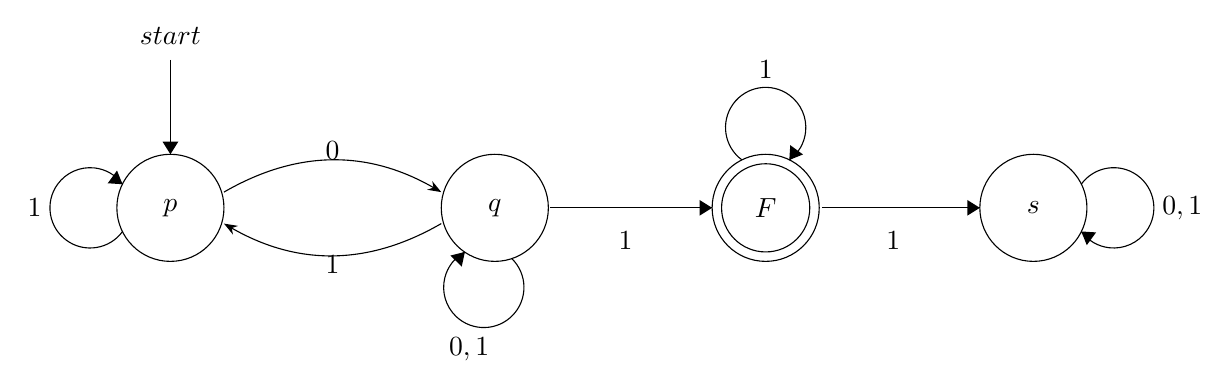
\begin{tikzpicture}[scale=0.2]
\tikzstyle{every node}+=[inner sep=0pt]
\draw [black] (9.1,-16.5) circle (3.4);
\draw (9.1,-16.5) node {$p$};
\draw [black] (29.7,-16.5) circle (3.4);
\draw (29.7,-16.5) node {$q$};
\draw [black] (46.9,-16.5) circle (3.4);
\draw (46.9,-16.5) node {$F$};
\draw [black] (46.9,-16.5) circle (2.8);
\draw [black] (63.9,-16.5) circle (3.4);
\draw (63.9,-16.5) node {$s$};
%\draw [black] (9.1,-3.6) circle (3.4);
\draw (9.1,-5.6) node {$start$};
%\draw [black] (12.8,-16.5) -- (26.3,-16.5);%p-q
\draw (12.5,-15.5) edge[bend left, above,-Stealth] node{0} (26.3,-15.5);
\draw (26.3,-17.5) edge[bend left, below,-Stealth] node{1} (12.5,-17.5); 
%\draw (18,-18) node [below] {$0$};
\draw [black] (33.2,-16.5) -- (43.5,-16.5);%q-f
\draw (38,-18) node [below] {$1$};
\fill [black] (43.5,-16.5) -- (42.7,-16) -- (42.7,-17);
\draw [black] (50.5,-16.5) -- (60.5,-16.5);%F-s
\draw (55,-18) node [below] {$1$};
\fill [black] (60.5,-16.5) -- (59.7,-16) -- (59.7,-17);
\draw [black] (9.1,-7.1) -- (9.1,-13.1);
\fill [black] (9.1,-13.1) -- (9.6,-12.3) -- (8.6,-12.3);
\draw [black] (6.063,-17.999) arc (-36:-324:2.55);
\draw (0.95,-16.5) node [left] {$1$};
\fill [black] (6.06,-15) -- (5.71,-14.13) -- (5.12,-14.94);
\draw [black] (30.768,-19.714) arc (46.11307:-241.88693:2.55);
\draw (28.07,-24.74) node [below] {$0,1$};
\fill [black] (27.8,-19.3) -- (26.88,-19.53) -- (27.6,-20.23);
\draw [black] (45.401,-13.463) arc (234:-54:2.55);
\draw (46.9,-8.35) node [above] {$1$};
\fill [black] (48.4,-13.46) -- (49.27,-13.11) -- (48.46,-12.52);
\draw [black] (66.937,-15.001) arc (144:-144:2.55);
\draw (72.05,-16.5) node [right] {$0,1$};
\fill [black] (66.94,-18) -- (67.29,-18.87) -- (67.88,-18.06);
\end{tikzpicture}
\end{center}
每一个state里面存在一个proposition,它表示这个proposition is hold at this state,自然地states就变成了possible worlds. state现在可以接受多个输入$\{0,1\}$,那么这里就表示我们有两个relations $\rho_0$和$\rho_1$,对应我们需要两个pair来构建不同的modality $(\square_0,\Diamond_0)$和$(\square_1,\Diamond_1)$,它们都是用于描述某个state的successor. 因此这里可以对应上一个Kripke structure, 对上图我们可以列举几个vaild formula.
$$
\begin{aligned}
&K \vDash \neg \Diamond_0 F && \text{does not end with 0} \\
&K \vDash p \to \Diamond_0 p &&\text{$p$ has a 1-loop} \\
&K \vDash \Diamond_0~true && \text{never stuck with input 0} \\
&K \vDash \Diamond_1~true && \text{never stuck with input 1} \\
\end{aligned}
$$
再看一个稍微复杂一点
$$
K \vDash F \to \Diamond_0(\neg \Diamond_0 F \wedge \neg \Diamond_1 F)
$$
它意思如果某个状态$\sigma$下$F$ is hold, 那么$\sigma$ accept 0 的successors $\{s_i\}$中每个$s_i$的successors都无法hold $F$,显然这是成立的. 
\end{annotation}


\begin{definition}
\rm A system $\mathcal{S}$ of proof rules and axioms of modal logic is sound iff, for all formulas $\psi$ and all sets of formulas $\Phi$:
$$
\Phi \vdash_S \psi~\text{implies}~\Phi \vDash_g \psi
$$
\end{definition}


\begin{annotation}
\rm 上述soundness实际在建立关于axiomatic modal logic和semantic modal logic之间的一座桥,这座桥需要每一个axiom make sense. 
\end{annotation}

\begin{lemma}
\rm Kripke axiom $\square(\phi \to \psi) \to (\square\phi \to \square\psi)$ is sound.
\end{lemma}

\begin{proof}
\rm 首先给定任意一个Kripke structure $K$. 我们需要证明
$$
K,s \vDash \square(\phi \to \psi) \to (\square\phi \to \square\psi).
$$
因此假设其前提
$$
\begin{aligned}
&K,s \vDash \square(\phi \to \psi) \\
&K,s \vDash \square\phi
\end{aligned}
$$
那么对应所有满足$s \rho t$的successor $t$, 都有
$$
\begin{aligned}
&K,t \vDash \phi \to \psi \\
&K,t \vDash \phi
\end{aligned}
$$
自然地这里有$K,t \vDash \psi$,于是$K,s \vDash \Diamond \psi$. 
\end{proof}

\begin{lemma}
\rm G\"{o}del Rule $\infer{\square\phi}{\phi}$ is sound.
\end{lemma}

\begin{proof}
注意这里的结论是建立在global assumption上的,即$K,s \vDash \phi$ for any $s \in W$,证明过程是显然的.
\end{proof}

\begin{lemma}
\rm A Kripke frame $(W,\rho)$ is reflexive, that $\rho$ is reflexive, if and only if $K,s \vDash \square q \to q$ for all Kripke structures $K = (W,\rho,v)$. 
\end{lemma}

\begin{proof}
($\Rightarrow$) 若$(W,\rho)$ is reflexive, 这是显然的.

($\Leftarrow$) 若$K,s \vDash \square q \to q$ for all Kripke structures $K = (W,\rho,v)$. 假设存在一个$r$ such that $(r,r) \notin \rho$, 构造一个比较巧妙地valuation $v$
$$
v(s)(q) = \left\{
\begin{aligned}
&true && \text{if}~r \rho s \\
&false && \text{otherwise}
\end{aligned}
\right.
$$
那么显然有$K,r \vDash \square q$,根据前提这里有$K,r \vDash q$,而根据valuation这里就$r$存在一个successor是它自己,即$(r,r)$与假设矛盾. 
\end{proof}

\begin{lemma}
\rm  A Kriple frame $(W,\rho)$ is transitive, that $\rho$ is transitive, if and only if $K,s \vDash \square q \to \square\square q$ for all Kripke structures $K=(W,\rho,v)$. 
\end{lemma}

\begin{proof}
\rm ($\Rightarrow$) 若$(W,\rho)$ is transitive, 给定$K,s \vDash \square q$,对于$s$的任意一个successor $t$($s \rho t$)则有$K,t \vDash p$,进一步对$t$的任意一个successor $r$($t \rho r$),考虑transitive $s \rho r$,那么有$K,r \vDash p$. 由于$t$和$r$的任意性,因此$K,s \vDash \square\square p$. 

($\Leftarrow$) 若Kriple frame满足对任意的valuation $v$都有$K,s \vDash \square q \to \square\square q$. 假设$(W,\rho)$不是transitive, 那么存在$r_1,r_2,r_3 \in W$ such that $r_1 \rho r_2, r_2 \rho r_3$ and $(r_1,r_3) \notin \rho$. 构造一个valuation $v$
$$
v(s)(q) = \left\{
\begin{aligned}
&true && \text{if}~r_0 \rho s \\
&false && \text{otherwise}
\end{aligned}
\right.
$$
那么$K,r_0 \vDash \square q$,但是因为$(r_0,r_3) \notin \rho$,因此$K, r_0 \nvDash \square\square q$,和假设前提矛盾了. 
\end{proof}

\begin{annotation}
\rm 这座需要两边的支撑一样高,给定特定axiomatic modal logic, 我们得到找到与之对应的semantic modal logic,我们的手法就是sketch it from basic Kripke frame. 当我们尝试构造了一部分之后,我们需要让其make sense,上述lemma利用formula来characterize是一个不错的选择. 
\end{annotation}

\begin{definition}
\rm (\redt{characterization})Let $C$ be a class of Kripke frames and $\phi$ a formula in modal logic.  Formula $\phi$ characterizes $C$, if for every Kripke frame $(W,\rho)$:
$$
(W,\rho) \in C ~\text{iff for each}~v: K,s \vDash \phi~\text{holds for}~K=(W,\rho,v).  
$$
\end{definition}

\begin{theorem}
\rm (\redt{soundness of $\mathcal{S}4$})The Kriple proof rules for $\mathcal{S}4$ are sound for the class of reflexive and transitive frames.
\end{theorem}

\begin{theorem}
\rm The conjunction of the following two multimodal formulas
$$
\begin{aligned}
&\square_a p \to (p \wedge \square_a\square_b p) \\
&\square_a(p \to \square_b p) \to (p \to \square_a p)
\end{aligned}
$$
characterizest the class of all multimodal kripke frames $(W, \rho_a,\rho_b)$ such that $\rho_a$ is the reflxive, transitive closure of $\rho_b$. 
\end{theorem}

\begin{proof}
\rm ($\Leftarrow$) 如果$(W, \rho_a, \rho_b)$is Kripke frame where $\rho_a$ is the reflexive, transitive closure of $\rho_b$. 对于一个formula只要注意到$\square_a\square_a p \to \square_a\square_b p$即可,可以从需要考虑的successors数量来证明. 对于第二个formula, 先给一个思考图
$$
% https://tikzcd.yichuanshen.de/#N4Igdg9gJgpgziAXAbVABwnAlgFyxMJZABgBoBGAXVJADcBDAGwFcYkQEBfU9TXfQigBMFanSat2ORGgAEAHXk4IC+XACOzegCcYAfQBGsuQD9FOGAA8cwemCicTxkN17Y8BIgHZRNBizZEEG0XHhAMdwEiABZSYjF-SSCAdz1gLE5Qt35PFABWOISJQJBU9IBqckzOMRgoAHN4IlAAM20IAFskMhBlJHI-YvY4VW0ACwhDAD0AKlkcLJA2zv6aPsQRcQCpUYnpuZDXJfauxABmNYgkWK2kkANEVKxdyaMyrErqsOXTgd6r840RhYMAlKD0OBjOogQbbIIGGaLH7XS5ITbA0HscGQ6Gwu4IpEnbqowH3GD2JBnHqJEojRTjV6zFyUThAA
\begin{tikzcd}
                                                                    &  &                                                                                            &  & w_{i} \arrow[r, "b:w_i \rho_b w_{i+1}"] & w_{i+1} \arrow[rrd, "b*", dashed] &  &   \\
s \arrow[rr, "s \rho_b^* t"] \arrow[rrrru, "s \rho_b^* w_i", bend left] &  & t:p \to \square_b p ~\text{and}~ p \arrow[rrrrr, "t \rho_b^* r"] \arrow[rru, "b*", dashed] &  &                                         &                                   &  & r
\end{tikzcd}
$$
这里$\rho_a  = \rho_b^*$. 这里证明手法是
$$
\square_a(p \to \square_b p) \to \square_a(p \to \square_a p) ~\text{and}~ \square_a(p \to \square_a p) \to (p \to \square_a p)   
$$
最重要是证明第一个implication,第二个implication是前面已经证明过的reflexive. 对于第一个implication它描述的是首先给出前提(1)$\square_a(p \to \square_b p)$即$s \rho_b^* t$. 然后我们想要将$t$中$p \to \square p$扩展至$p \to \square_b^* p$,因此再给一个假设前提$t$ holds p,我们来考察$\square_b^* p$是否成立即$t \rho_b^* r$. 这里我们需要分解$t \rho_b^* r$使其为$w_i \rho_b w_{i+1}$ for all $i < n$,其中$w_0=t$和$w_{n} = r$. 利用数学归纳法证明$K,w_i \vdash p$,这里就不详细描述了,和后面一个证明过程类似,但是说明几点: (1)$s \rho_b^* w_i$送来了$p \to \square_b p$ (2)假设前提保证了$K,w_i \vDash p$. 因此$K,w_{i+1}\vDash p$. 

($\Rightarrow$) 如果$(W, \rho_a, \rho_b)$is Kripke frame such that above formulas are vaild in it for any valution $v$. 我们得证明$\rho_a = \rho_b^*$. 这种证明两个集合相等的手法,还是用两边证.

先证\bluet{$\rho_a \subseteq \rho_b^*$}. 取任意的$(s,t) \in \rho_a$,我们得证明$(s,t) \in \rho_b^*$. 还是构造一个特殊的valuation
$$
v(w)(q) = \left\{
\begin{aligned}
&true && \text{if}~(s,w) \in \rho_b^* \\
&false && \text{otherwise}
\end{aligned}
\right.
$$
我们的思路是首先证明第二个formula的前提(1) $\square_a(p \to \square_b p)$,从而得到对应的conclusion (2) $(p \to \square_a p)$,由给定的$v$结合$\rho_b^*$的reflexive性质,自然地有$K,s \vDash p$,在使用一下(2)得到$K,t \vDash p$, 这样就有$(s,t) \in \rho_b^*$.  证明(1)思路是依然是假设前提: 给定$s \rho_a w$且$K,w \vDash p$,实际上$(s,w) \in \rho_b^*$. 考虑下面的思考过程
$$
% https://tikzcd.yichuanshen.de/#N4Igdg9gJgpgziAXAbVABwnAlgFyxMJZABgBpiBdUkANwEMAbAVxiRAQF9T1Nd9CUAJnJVajFmwDuiAARoQXHtjwEiAFhHV6zVohCSA5AtEwoAc3hFQAMwBOEALZIyIHBCQBGLeN0g6suBkAHSDbAAsIAH0AIwA9ACoZSRBqBjpomAYABV4VARAGGGscBW4QO0dnajckYTEdNkCQ8Ki4xMMUgvTMnOV+NkLizoywKCQAZmJFcvsnRC9Xd0Q67Qk9aNlJZoiYhI7U7uzc-r1Bko4KDiA
\begin{tikzcd}
s \arrow[rr, "a: s \rho_b^* w"] \arrow[rrrr, "s \rho_b^* w'", bend left] &  & w: p \arrow[rr, "b: w\rho_b^*w'"] &  & w'
\end{tikzcd}
$$
另外又给了一个$w'$满足$w \rho_b w'$,再根据$\rho_b^*$的transitive得到$s \rho_b^* w'$,从而$K,w' \vDash p$. 

再证\bluet{$\rho_a \supseteq \rho_b^*$}. 取任意的$(s,t) \in \rho_b^*$,我们要证明$(s,t) \in \rho_a$. 依然构造一个类似的valuation
$$
v(w)(q) = \left\{
\begin{aligned}
&true && \text{if}~(s,w) \in \rho_a \\
&false && \text{otherwise}
\end{aligned}
\right.
$$
我们的思路: 由于我们构造地特别的$v$有$K,s \vDash \square_a p$, 借助命题中的第一个formula得到对应的conclusion (1) $K,s \vDash p \wedge \square_a\square_b p$. 考虑下面的思考过程
$$
% https://tikzcd.yichuanshen.de/#N4Igdg9gJgpgziAXAbVABwnAlgFyxMJZABgBoBGAXVJADcBDAGwFcYkQ5E0QBfU9TLnyEUAJlLFqdJq3YB3APpYuvfiAzY8BIgFYKUhizaIQOFXwGbhRAMwSDM4yEXAsAanI9zUmFADm8ESgAGYAThAAtkhkphBI4tJG7HAABAA6aaEAFhAKAEYAegBUKTiqIeFRiDE4cYjkNIxYYE5Q9HBZviA0eTBgUEg2xBYgYZFIDbGDPX0D1TSGsiZ5iCmKWOmZOflrCq4ePOWjldNTiAlNLextHV0z-YPDlDxAA
\begin{tikzcd}
                                                                 &  & w_i:p \arrow[r, "b: w_i \rho_b w_{i+1}"] & w_{i+1}:p \arrow[rrd, dashed, bend left] &  &     \\
s:p \arrow[rrrrr, "s \rho_b^* t"] \arrow[rru, dashed, bend left] &  &                                          &                                          &  & t:p
\end{tikzcd}
$$
我们考虑将$s \rho_b^* t$拆开,设$w_i \rho_b w_{i+1}$ for all $i < n$,其中$w_0 = s$和$w_n = t$,这是可以做到的,考虑closure的构造过程. 再用一下数学归纳法证明$K, w_i \vDash p$,在$i=0$显然是成立的,假设$w_i$成立,那么根据$v$即有$s \rho_a w_i$,再利用一下(1)可以得到$K,w_i \vDash \square_b p$,因此$K,w_{i+1} \vDash p$. 最终$K,t \vDash p$,那么$(s,t) \in \rho_a$. 
\end{proof}

\begin{annotation}
\rm \bluet{回顾上面的证明手法},我们如果想要刻画两个possible worlds是否存在某种关系,例如$(r,t) \stackrel{?}{\in} \rho$,我们可以额外借助一个formula $p$和valuation $v$,仅使得所有$w$满足$r \rho w$都hold $p$. 这样如果我们能利用额外和$p$相关的条件间接证明$t$ holds $p$, 那么就可以证明$s \to t$. 我们应该意识到relations是Kripke frame固有的性质,与valuation无关因此这里我们可以任意的定义它.  
\end{annotation}

\newpage
\section{Natural Deduction}

\begin{remark}
\rm \redt{Natural deduction is a kind of proof calculus in which logical reasoning is expressed by inference rules closely related to the "natural" way of reasoning}. 
\end{remark}

\subsection{Judgments and Propositions}

\begin{definition}
\rm A \emph{judgment} is somthing we may know, this is, an object of knowledge. A judgment is \emph{evident} if we in fact know it.
\end{definition}

\begin{annotation}
\rm "A is false" (see classical logic), "A is true at time t" (see temporal logic), "A is necessarily true" or "A is possibly true" (see modal logic), "the program M has type τ" (see programming languages and type theory), "A is achievable from the available resources" (see linear logic). 
\end{annotation}

%inference rule 写一遍没意思

\subsection{Introduction and Elimination}

\begin{definition}
\rm Inference rules that introduce a logical connective is the conclusion are known as \emph{introduction rules}. i.e., to conclude "$A~\text{and}~B~true$" for propositions $A$ and $B$, one requires evidence for "$A~true$" and $B~true$. As an inference rule:
$$
\infer[\wedge I]{A \wedge B ~true}{A~true & B~true}
$$
Here $\wedge I$ stands for "conjunction introduction".
\end{definition}

\begin{annotation}
\rm 实际上面的inference rule的general form应该是
$$
\infer[\wedge I]{A \wedge B ~true}{A~prog & B~prog & A~true & B~true}
$$
这里才能帮助后面的$\vDash$ make sense. 
\end{annotation}

\begin{definition}
\rm Inference rules that describe how to deconstruct information about a compound proposition into information about its consitiuents are elimination rules. i.e., from $A \wedge B~true$, we can conclude $A~true$ and $B~true$:
$$
\infer[\wedge E_L]{A~true}{A \wedge B ~true}~~~~~~\infer[\wedge E_R]{B~true}{A \wedge B ~true} 
$$
\end{definition}

\begin{annotation}
\rm The meaning of conjunction is determinded by its \emph{verifications}.  
\end{annotation}

\subsection{Hypothetical Derivations}

\begin{definition}
\rm A \emph{hypothetical judgment} is $J_1, \cdots, J_n \vdash J$, where judgments $J_1,\cdots,J_n$ are unproved assumptions, and the judgment $J$ is the conclusion. A \emph{hypothetical deduction}(derivation) for $J_1, \cdots, J_n \vdash J$ has the form 
$$
\deduce[\vdots]{\raisebox{-1.0em}{$J$}}{J_1 & \cdots & J_n}
$$
which means $J$ is derivable from $J_1, \cdots, J_n$. 
\end{definition}

\begin{annotation}
\rm 上面的$J_1,\cdots,J_2$都可以替换成关于$J_i$的一个hypothetical derivation. 
\end{annotation}


\begin{definition}
\rm In the natural deduction calculus, an assumption is discharged when the conclusion of an inference does not depend on it, although one of the premises of the inference does\cite{tln}.
\end{definition}

\begin{annotation}
\rm Once the appropriate rules have been completed, these are known as discharged assumptions, and are not included in the pool of assumptions on which the conclusion of the rule depends\cite{discharged-proofwiki}.
\end{annotation}

\begin{annotation}
\rm hypothetical derivation要求最后的conclusion依赖的poof of assumptions不是空的. 
\end{annotation}

\begin{theorem}
\rm \redt{Deduction theorem} \[T, P \vdash Q \iff T \vdash P \to Q\].
\end{theorem}

\begin{annotation}
\rm 在deduction theorem中我们注意到第一个hypothetical judgment里面的antecedent $Q$被去掉了,在第二个hypothetical judgment的succedent里面作为一个implication的antecedent出现了,这里我们就可以说assumption $Q$ is discharged,即现在的conclusion已经不依赖它了. 那么我们是如何构造deduction theorem里面的implication的呢? 下面接着看
\end{annotation}

\begin{definition}
\rm (\redt{implication}) If $B$ is true under the assumption that $A$ is true, formly written $A \supset B$. The corresponed introduction and elimination rule as follow \[\infer[\supset\!\!I^u]{A \supset B~true}{\deduce[\vdots]{B~true}{\infer[u]{A~true}{}}}~~~~~ \infer[\supset\!\!E]{B~true}{A\supset B~true & A~true}\]
\end{definition}

\begin{annotation}
\rm \redt{Why indexed $u$} In the introduction rule, the antecedent named $u$ is discharged in the conclusion. This is a mechanism for delimiting the scope of the hypothesis: its sole reason for existence is to establish "$B~true$"; it cannot be used for any other purpose, and in particular, it cannot be used below the introduction.

上面这段话出自natural deduction的wiki,这个$u$scope了assumption $A~true$的开端,因为$A\supset B$并不依赖$A~true$, 它描述只是if $A~true$ then $B~true$. 
同时最后的introduction rule会将这个assumption $A~true$ discharged掉,表示scope在这里已经结束了. 而implication rule会将上述derivation直接总结得到一个结论,即
$$
A \vdash B \Rightarrow \cdot\vdash A \to B. 
$$
\end{annotation}

\begin{example}
\rm Considering the following proof of $A \supset (B \supset (A \wedge B))$
$$
\infer[I^u]{A \supset (B \supset (A \wedge B))~true}{\infer[I^w]{B \supset (A \wedge B)~true}{\infer[\wedge I]{A \wedge B~true}{\infer[u]{A~true}{} & \infer[w]{B~true}{}}}}.
$$

这整个derivation不是hypothetical的,因为两个assumptions $A~true$和$B~true$都已经被discharged,因此它实际上一个complete proof! 
\end{example}

\begin{definition}
\rm (\redt{disjunction}) The elimination rule for disjunction:
$$
\infer[\vee E^{u,w}]{C~true}{A \vee B ~true & \deduce[\vdots]{C~true}{\infer[u]{A~true}{}} & \deduce[\vdots]{C~true}{\infer[w]{B~true}{}}}
$$
both assumption $u,w$ are discharged at the disjunction elimination rule. 
\end{definition}


\begin{definition}
\rm The falsehood elimination rule:
$$
\infer[\perp\!\!E]{C~true}{\perp~true}
$$
\end{definition}

\begin{annotation}
\rm falsehood elimination的意义在哪? 首先你应该主要到一个特殊等价命题$A \vee \perp = A$,从$\vee$的introduction rule来看这意味$\perp~true \vdash A~true$,由于$A$是任意的,因此我们得到了$\perp~true \vdash C~true$. 
\end{annotation}

\newpage
\subsection{Harmony}

\begin{definition}
\rm \redt{Local soundness} shows that the elimination rules are not strong: no matter how we apply eliminations rules to the result of an introduction we cannot gain any new information.
\end{definition}

\begin{definition}
\rm \redt{Local completeness} shows that the elimination rules are not weak: there is always a way to apply elimination rules so that we can reconstitute a proof of the original proposition from the the results by apply intruduction ruls. 
\end{definition}

\begin{annotation}
\rm local soundness告诉你通过elimination得到的东西不会比你已经知道的东西强(not strong),而local completeness告诉你可以利用通过elimination得到的东西来构造你原本你已经知道的东西(not weak). 
\end{annotation}


\begin{definition}
\rm Given two deduction of same judgment, we use the notion
$$
\deduce{A~true}{\mathcal{D}} \Longrightarrow_{R} \deduce{A~true}{\mathcal{D'}} 
$$
for the \redt{local reduction} of a deduction $\mathcal{D}$ to another deduction $D'$ of same judgement $A~true$. Simliarly, we have \redt{local expansion}
$$
\deduce{A~true}{\mathcal{D}'} \Longrightarrow_{E} \deduce{A~true}{\mathcal{D}}
$$
\end{definition}


\begin{definition}
\rm (\redt{substitution Principle}) If 
$$
\deduce[\mathcal{E}]{C~true}{\infer[u]{A~true}{}}
$$
is a hypothetical proof of $\mathcal{C}~true$ under the undischarged hypothesis $A~true$ labelled $u$, and 
$$
\deduce{A~true}{\mathcal{D}}
$$
is a proof of $A~true$ then
$$
\deduce[\mathcal{E}]{C~true}{\infer[u]{A~true}{\mathcal{D}}}
$$
is our notation for substituting $\mathcal{D}$ for all uses of the hypothesis labelled $u$ in $\mathcal{E}$. This deduction, also sometime written as $[\mathcal{D}/u]\mathcal{E}$ no longer depends on $u$.  
\end{definition}


\begin{example}
\rm If given a elimination rule of disjunction as follow
$$
\infer[\vee\!E_L]{A~true}{A \vee B~true}
$$
The rule a little bit stronger, since we would not be able to reduce
$$
\infer[\vee\!E_L]{A~true}{\infer[\vee\!I_R]{A \vee B~true}{B~true}}
$$
As u can see it's not local soundness. 
\end{example}


%\begin{definition}
%\rm The \redt{soundness} of proof system will assure that we can %only construct proofs of vaild arguments. That is, we want to %prove that every sentence in a proof is entailed by previous %sentenses. 
%\end{definition}

%Godel
%\begin{definition}
%\rm A deduction system is said to be complete if every %universally valid formula in the language $L$ has a proof under %the proof system.
%\end{definition}




\newpage
\subsection{Verifications and Uses}

\begin{definition}
\rm a verification should be a proof that only analyzes the consitituents of a proposition.
\end{definition}


\begin{annotation}
\rm \cite{15-317-vu} 在natural deduction中由于local reduction的存在,可能会让一个证明过程变得非常的冗余,例如在证明conjunction commutativity
$$
\infer[\supset I^u]{(A \wedge B) \supset (B \wedge A)~true}{\infer[\wedge I]{B \wedge A~true}{\infer[\wedge E_2]{B~true}{\infer[\wedge I]{A \wedge B~true}{\infer[\wedge E_1]{A~true}{\infer[u]{A \wedge B ~true}{}}  &  \infer[\wedge E_2]{B~true}{\infer[u]{A \wedge B ~true}{}}}}  &  \infer[\wedge E_1]{A~true}{\infer[u]{A \wedge B ~true}{}}}}
$$
其中左上角的local reduction显然是冗余的. 这样对于谈论某个具体proposition的proof时就会出现问题,因为the shape of proof is not decidable. 同时我们也希望未来能够设计出一个tool用于deviates proofs automatically,也就是search proof automatically. 因此从natural deduction上诞生了一个新的calculus,它会在syntax level上来施加一些限制,借此限制the shape of proof. 最后我们将证明这个calculus引入的restrictions不会产生side-effect.   
\end{annotation}


\begin{definition}
\rm Writing $A\uparrow$ for the judgment "A has a verification". Naturally, this should mean that $A$ is true,  and that the evidence for that has a special form.
\end{definition}

\begin{definition}
\rm Writing $A\downarrow$ for the judgment "A may be used". $A\downarrow$ should be the case when either $A~true$ is a hypothesis, or $A$ is deduced from a hypothesis via elimination rules. 
\end{definition}

\begin{annotation}
\rm 我觉得下述两种理解方式更为明确易懂
\begin{itemize}
	\item $A \uparrow$ denotes that we are searching for a verfication of $A$;
	\item $A  \downarrow$ denotes that we are allowed to use $A$. 
\end{itemize}
\end{annotation}

\begin{annotation}
\rm 上述两个definitions里面隐藏着非常重要但有点不正式的结论:If $A$ has a vertification then $A$ true, 反之依然. 后面我们将形式化地证明它们. 
\end{annotation}

\begin{definition}
\rm For conjunction. 
$$
\begin{aligned}
&\infer[\wedge I]{A \wedge B\uparrow}{A \uparrow & B \uparrow} &&& \infer[\wedge E_L]{A \downarrow}{A \wedge B \downarrow} &&&& \infer[\wedge E_R]{B \downarrow}{A \wedge B \downarrow}
\end{aligned}
$$
\end{definition}


\begin{definition}
\rm For implication
$$
\begin{aligned}
&\infer[\supset^u]{A \supset B \uparrow}{\deduce[\vdots]{B\uparrow}{\infer[u]{A\downarrow}{}}} &&& \infer[\supset E]{B \downarrow}{A \supset B \downarrow & A \uparrow}
\end{aligned}
$$
\end{definition}

\begin{annotation}
\rm (\redt{why implication}) In order to have a verification of $A \supset B$, we need a proof of $B$ and we are given an assumption $A$ to work with. Therefore, we will need a verification of $B$ and we are allowed to use $A$. 

When using an implication statement in a proof, we need to show that the antecedent holds, so we need a verification of it. Only then we are allowed to use the consequent.
\end{annotation}

\begin{example}\label{use-is-weaker}
\rm
$$
\infer{((A \supset A) \supset B) \supset B \uparrow}{\infer{B ~?}{(A\supset A) \supset B ~? & \infer{A \supset A ~?}{\infer{A~?}{A~?}}}}
$$
\end{example}

\begin{example}\label{early-verification-and-truth}
\rm 
$$
\infer[\supset I^u]{(A \wedge B) \supset A~true}{\infer[\wedge E_L]{A~true}{\infer[u]{A\wedge B~true}{}}}
$$
那么它对应上verification和use
$$
\infer[\supset I^u]{(A \wedge B) \supset A~?}{\infer[\wedge E_L]{A \downarrow}{A \wedge B \downarrow}}
$$
一切都非常奇怪,这个verification和use到底是怎样对应truth? 从前面两个例子都可以清晰地感觉到一个阻力,即
$$
\deduce[???]{A \uparrow}{A \downarrow}
$$
就是当我们在use $A$的时候,实际上存在一个$A$ has a verification. 
\end{example}


\begin{definition}
\rm For disjunction
$$
\begin{aligned}
&\infer[\vee I_L]{A \vee B \uparrow}{A \uparrow} &&& \infer[\vee I_R]{A \vee B \uparrow}{B \uparrow} &&&  \infer[\vee E^{u,w}]{C \uparrow}{A \vee B \downarrow & \deduce[\vdots]{C\uparrow}{\infer[u]{A\uparrow}{}} & \deduce[\vdots]{C\uparrow}{\infer[w]{B\downarrow}{}}}
\end{aligned}
$$
\end{definition}


\begin{definition}
\rm For truth and falsehood.
$$
\begin{aligned}
& \infer[\top I]{\top \uparrow}{} &&& \infer[\perp E]{C\uparrow}{\perp \downarrow}
\end{aligned}
$$
\end{definition}

\begin{annotation}
\rm $\perp \downarrow$ signifies a contradiction from our hypotheses.
\end{annotation}

\begin{annotation}
\rm the elimination rule of disjunction and falsehood里面出现conclusion $C \uparrow$也很奇怪,为什么不是$C \downarrow$?
\end{annotation}

\begin{definition}\label{arrow switch of atomic}
\rm For atomic propositions.
$$
\infer[\downarrow\uparrow]{P \uparrow}{P \downarrow}.
$$
\end{definition}

\begin{annotation}
\rm 当引入上述的arrow switch之后我们可以回答前面的种种问题了. 首先是example \ref{use-is-weaker},假设其中的$A,B$都是atomic proposition,则
$$
\infer[\supset I^w]{((A \supset A) \supset B) \supset B \uparrow}{\infer[\downarrow\uparrow]{B \uparrow}{\infer{B ~\downarrow}{\infer[w]{(A\supset A) \supset B ~\downarrow}{} & \infer[\supset I^u]{A \supset A ~\uparrow}{\infer[\downarrow\uparrow]{A~\uparrow}{\infer[u]{A~\downarrow}{}}}}}}
$$
同时如果将implication emilination的premise换成$A \downarrow$,在找$A \supset A \downarrow$的proof时就被卡住了. example \ref{early-verification-and-truth}类似. 那么有一个很自然的问题这个arrow switch能不能推广到任意的propositions上呢? 本质上是没有问题的,例如
$$
\infer[\supset I^u]{A \supset A \uparrow}{\infer[\downarrow\uparrow]{A \uparrow}{\infer{A \downarrow}{A \supset A \downarrow & \infer[\downarrow\uparrow]{A \uparrow}{\infer[u]{A~\downarrow}{}}}}}
$$
但是这样的语法又会使得proof search space变大,并不符合我们的初衷,因此我们只将arrow switch放在的了atomic proposition上,这样做的后果你也可以看到,需要将connectives都展开.  

再来思考另外一种arrow switch
$$
\infer[\uparrow\downarrow]{F \uparrow}{&F \downarrow&}
$$
这个人在本质上也是没有问题的,当我们有一个关于$F$的verification,我们当然可以use it. 但是引入它同样会造成我们的proof search space,就像classical logic中的tautologies,我们可以在任何proof中使用它,但是有时候是没有意义的. 同在emilinotation rule of disjunction and falsehood中的conclusion中我们都是使用的verification,而不是use,也是为了防止后续使得我们的proof变得复杂. 
\end{annotation}

\begin{theorem}
\rm (\redt{Global Soundness}) $\deduce[\vdots]{\text{If}~A \uparrow~\text{and}~C\uparrow~\text{then}~C \uparrow}{A \downarrow}$
\end{theorem}

\begin{annotation}
\rm Global Soundness意味着如果if the verification formula of $C$ under the verification formula $A$,那么在$C$中使用$A$,并不会得到任何其他new informations.
\end{annotation}

\begin{theorem}
\rm (\redt{Global Completeness}) If $A \downarrow$, then $A \uparrow$. 
\end{theorem}

\begin{annotation}
\rm Global completeness意味着如果我们确定formula $A$在某种情况下可以使用,那么在相同的assumptions下我们可以推导出一个关于它的verification. 这在前面关于$\downarrow\uparrow$转换规则的annotation中已经见识过一个特殊例子了. 
\end{annotation}

\newpage
\subsection{Notational Definition}

\begin{definition}
\rm A \redt{notational definition} gives the meaning of the general form of a proposition in terms of another proposition whose meaning has already been defined.
\end{definition}

\begin{example}
\rm We can define logical equivalence, written $A \equiv B$ as 
$$
(A \supset B) \wedge (B \supset A).
$$ 
\end{example}

\begin{example}
\rm We can define negation $\neg A$ as 
$$
\neg A = (A \supset \perp) \Longrightarrow \infer[\neg I]{\neg A}{\deduce[\vdots]{\perp}{A}}
$$
We also can give the introduction rule of falsehood.
$$
\infer[\perp I]{\perp}{\neg A & A}
$$
so $\perp$ actually means any contradictions. moreover double negation is coming.
\end{example}

\begin{annotation}
\rm notaional definition可以看做用已有的东西构造出一些东西. 与之对应的是我们可以直接符号化的给出某个新的定义,称之为symbolic definition. 
\end{annotation}

\newpage
\subsection{Soundness and Completeness of Native Natural Deduction}

\begin{definition}
\rm \cite{cs245-nd}\redt{Soundness} of natural deduction means that the conclusion of proof is always a logical consequence of the premises. That is
$$
\text{If}~\Sigma \vdash \alpha, \text{then}~\Sigma \vDash \alpha. 
$$ 
\end{definition}


\begin{definition}
\rm \redt{Completeness} of natural deduction means that all logical consequences in propositional logic are provable in natural deduction. That is,
$$
\text{If}~\Sigma \vDash \alpha, \text{then}~\Sigma \vdash \alpha.
$$ 
\end{definition}

\begin{annotation}
\rm 其中$\Sigma \vdash \alpha$, 表示存在一个以$\Sigma$作为premise得到conclusion为$\alpha$的proof. 而$\Sigma \vDash \alpha$,就考虑两端的proposition加上truth-falsehood了, 即如$\Sigma^t = True$则有$\alpha^t = True$.

对于soundness的证明,我们需要根据$\alpha$的结构来做归纳,而后再考虑赋予其true/false来考虑. 这里记录一下对于结构归纳它是怎样对应一般归纳法命题$P(n)$结构上,这里的$n$应该对应$\alpha$的bottom-up derivation里面的maximum depth of line. 

而对于completeness的证明,相对来说会复杂一点. 我们需要下面3个lemma. 有一个疑问不引入negation是不是还说明不了completeness?
\end{annotation}

\begin{lemma}
\rm If $\Sigma =\{\alpha_0,\alpha_1,\cdots,\cdots,\alpha_n\} $ and $\Sigma \vDash \beta$, then
$$
\emptyset \vDash (\alpha_0 \to (\alpha_1 \to (\cdots \to (\alpha_n \to \beta)\cdots)).
$$
\end{lemma}

\begin{annotation}
\rm Deduction theorem体现的淋漓尽致,将$\beta$完美转换成了一个tautology. 
\end{annotation}

\begin{lemma}\label{how-to-construct-provable-formula}
\rm For any well-form formula $\gamma$ containing atoms $p_1,p_2,\cdots,p_n$ and any valuation $t$, we have 
\begin{enumerate}
	\item If $\gamma^t = True$ then $\widehat{p}_1,\widehat{p}_2,\cdots,\widehat{p}_n \vdash \gamma$;
	\item If $\gamma^t = False$ then $\widehat{p}_1,\widehat{p}_2,\cdots,\widehat{p}_n \vdash \neg\gamma$;
\end{enumerate}
where defines $\widehat{p}_i$ as follow
$$
\widehat{p}_i = \left\{
\begin{aligned}
&p_i && \text{if}~p_i^t = True \\
&\neg p_i && \text{if}~p_i^t = False
\end{aligned}
\right.
$$
\end{lemma}

\begin{example}
\rm 若$\gamma = p \to q$,我们可以构造一个真值表
\begin{center}
\begin{tabular}{|c|c|c|c|}
\hline
$p$ & $q$ & $p \to q$ & Claim \\ 
$T$ & $T$ & $T$ & $p , q \vdash p \to q$ \\
$T$ & $F$ & $F$ & $p , \neg q \vdash \neg(p \to q)$ \\
$F$ & $T$ & $T$ & $\neg p , q \vdash p \to q$ \\
$F$ & $F$ & $T$ & $\neg p , \neg q \vdash p \to q$ \\ 
\hline
\end{tabular}
\end{center}
那么上面的claims是怎么来的呢?我们可以来分别证明, 对于第一行
$$
\infer[u]{p \to q~true}{\infer{q~true}{\infer[u]{p~true}{} & q~true}}
$$
感觉有点奇怪,这里需要用到vars inference rule, 这里相对于对$q \vdash p \to q$的weaken premise. 对于第二行
$$
\infer[u]{\neg (p \to q)~true}{\infer{\perp}{\infer{q}{\infer[u]{p \to q~true}{} & p~true} & \neg q ~true}}
$$
对于第三行
$$
\infer[u]{p \to q~true}{\infer{q~true}{\infer{\perp}{\infer[u]{p~true}{} & \neg p ~true}}}
$$
对于第四行,和第三行类似. 可以看的出来这个lemma非常深刻,\bluet{只要将atoms调整为在当前valuation下都是true的命题,结论再对应调整,就可以构造一个对应的proof}. 
\end{example}

\begin{lemma}\label{tautologies-are-provable}
\rm For any well-formed formula $\gamma$, if $\emptyset \vDash \gamma$, then $\emptyset \vdash \gamma$. 
\end{lemma}

\begin{annotation}
\rm Lemma \ref{tautologies-are-provable}一句话概况就是tautologies are provable. 其证明过程可以用Lemma \ref{how-to-construct-provable-formula}来说明. 现在$\gamma$是一个tautology,那么对于所有的valuation都有$\gamma^t = true$,这有什么用呢? 这里还需要引入另外一种tautology $p \vee \neg p$,配合emilination rule of $vee$,即
$$
\infer{\gamma}{(p_1 \vee \neg p_1) & (p_2 \vee \neg p_2) & \cdots & (p_n \vee \neg p_n)&\deduce[\vdots]{\gamma}{\infer{}{\infer{p_1}{} & \cdots & \infer{p_n}{}}} & \cdots & \deduce[\vdots]{\gamma}{\infer{}{\infer{\neg p_1}{} & \cdots & \infer{\neg p_n}{}}}}
$$
这里需要考虑有$2^n$个cases,每一个对应一种valuation,又因为$\gamma$是tautology,因此最后的conclusion也都是$\gamma$. 
\end{annotation}

\begin{lemma}
\rm If $\emptyset \vdash (\alpha_0 \to (\alpha_1 \to (\cdots \to (\alpha_n \to \beta)\cdots))$, then $\{\alpha_0, \alpha_1,\cdots,\alpha_n\} \vdash \beta$, that is, $\Sigma \vdash \beta$. 
\end{lemma}

\newpage
\subsection{Derived Rules of Inference}

\begin{example}
\rm 
$$
\infer{A \supset C~true}{A \supset B~true & B \supset C~true}
$$
is a derived rule of inference. Its derivation is the following:
$$
\infer[\supset I^u]{A \supset C~true}{\infer[\supset E]{C~true}{B \supset C~true & \infer[\supset E]{B~true}{A \supset B~true & \infer[u]{A~true}{}}}}
$$
\end{example}

\begin{annotation}
\rm 关于derivation的推导这里有一些strategies在里面
\begin{itemize}
	\item 使用introduction rule从下至上,即我们想要什么;
	\item 使用elimination rule从上至下,即我们知道什么.
\end{itemize}
\end{annotation}

\begin{example}
\rm Modus tollens(这玩意不就是逆否命题)
$$
\infer[MT]{\neg A}{A \to B & \neg B}.
$$
\end{example}


\newpage
\subsection{Curry-Howard Conrrespondence}

\begin{definition}
\rm Curry-Howard correspondence is between the natural deduction and simply-typed $\lambda$-calculus at three levels
\begin{itemize}
	\item propositions are types;
	\item proofs are programs; and
	\item simplification of proofs is evaluation of programs.
\end{itemize}
That is
\begin{center}
\begin{tabular}{c|c}
Types & Propositions \\
\hline
Unit types (1) & Truth ($\top$)\\
\hline
Product type ($\times$) & Conjunction ($\wedge$) \\
\hline
Union type ($+$)& Disjunction ($\vee$) \\
\hline
Function type ($\to$) & Implication ($\supset$)\\
\hline
Void types (0) & False ($\perp$)
\end{tabular}
\end{center}
Every typing rule has a correspondence with a deduction rule. 
\end{definition}


\begin{example}
\rm The typing derivation of the term $\lam{a}{\lam{b}{\left<a,b\right>}}$ can be seen as a deduction tree proving $A \supset B \supset A \wedge B$.
\[
\begin{aligned}
	\infer[abs]{\Gamma\vdash\lam{x:A}{\lam{y:B}{\left<x,y\right>}}:A \to B \to A \times B}{\infer[abs]{\Gamma\vdash \lam{y:B}{\left<a,y\right>}:B \to A \times B}{\infer[pair]{\Gamma\vdash \left<a,b\right>: A \times B}{\infer[var]{\Gamma\vdash a:A}{a:A \in \Gamma} & \infer[var]{\Gamma\vdash b:B}{b:B \in \Gamma}}}} & \iff & 
	\infer[\supset I^u]{A \supset B \supset A \wedge B~true}{\infer[\supset I^w]{B \supset A \wedge B~true}{\infer[\wedge \wedge I]{A \wedge B ~true}{\infer[u]{A~true}{} & \infer[w]{B~true}{}}}}		
\end{aligned}
\]
\end{example}

\begin{annotation}
\rm 从上面例子中看的出来,the inference rule of natural deduction缺点什么,我也可以给原本每个inference rule都加上the annotation for proof terms. \cite{FP-pap}那么这里$M:A$有两种解释:
\begin{enumerate}
	\item $M$ is proof term for proposition $A$;
	\item $M$ is a program of type $A$. 
\end{enumerate}
这样解释Curry-Howard ismorphism或许方便一点. 让proof terms make sense: 我们有"if $M:A$ then $A~true$",反过来"if $A~true$ then $M:A$". 例如我们可以将the proof term of $A \wedge B~true$看做一个pair包含两个subterm,一个关于$A~true$和另一个关于$B~true$.
$$
\infer[\wedge I]{\left<M,N\right>: A \wedge B}{M:A & N:B}
$$
那么the elimination rule of conjunction对应一个natural projection.
$$
\begin{aligned}
\infer[\wedge E_L]{\pi_1 M:A}{M:A \wedge B} &&& \infer[\wedge E_R]{\pi_2 M:B}{M:A \wedge B} 
\end{aligned}
$$ 
\end{annotation}


\begin{example}
\rm 通过Curry-Howard isomorphism我们可以将我们想要证明的judgment转换到type system中,你会看到非常的便利! 例如
$$
(A \supset (B \wedge C)) \supset (A \supset B) \wedge (A \supset C)~true
$$
等价于
$$
\lam{x}{\left<\lam{y}{\pi_1(x~y)},\lam{y}{\pi_2(x~y)} \right>}: (A \to B \times C) \to (A \to B) \times (A \to C)
$$
一个implication被转换成了对应的abstraction,此时我们肯定会想如果给一个false proposition是不是就转不了? 例如
$$
(A \supset B) \supset (B \supset A)
$$
显然我们无法在现有type system构造出一个合理的abstraction使得$(A \to B) \to (B \to A)$.

迎面走来的问题是: 给定一个proposition true, 是否有其他的term with type和它对应呢? 显然是有的,
$$
\lam{z}{\lam{x}{\left<\lam{y}{\pi_1(x~y)},\lam{y}{\pi_2(x~y)} \right>}}z'
$$
那这是不是违反Curry-Howard isomorphsim了呢? 其实并不是,这里的对应是指proof terms和deduction of proposition true,  显然deduction变了,对应的proof terms也要变. 
\end{example}

\begin{annotation}
\rm Curry-Howard isomorphism建立在ND和STLC之间似乎看起来局限性很强,但是它是非常重要的第一步,是我们以另外一种视角来看待问题的方法,例如well-type term is normalizing,那么也意味well-formed formula is derivable. 之后researcher渐渐地发现了其他的logics也可以找到与之对应的programming language, 直到现在这仍然是一个active research field.
\end{annotation}

\newpage
\subsection{Quantifier}

\begin{annotation}
\rm natural deduction很自然地建立在propositional logic上,现在要把quantifier加到里面,我们就得面向first order logic了,这里需要引入terms和variables来为后面construction做准备. 另外还得必要引入关于term的properties,这里我们给它一个合适的名字叫做type, 即type of term, 为什么要引入这个它呢? 因为你可以想象我们经常在谈及quantified statement的时候,例如"every natural number is even or odd", 这里谈论的对象是natural number,那么这个natural number实际上就是这里term的type. 
\end{annotation}


\begin{definition}
\rm A formula $\forall x. A$ hold if and only if for every term $a$ chosen, the proposition $A[a/x]$ hold, where the proposition means all occurrences of $x$ in $A$ replaced by $a$. 
\end{definition}


\begin{definition}
\rm The introduction rule of universal quantifier is defined as follow:
$$
\infer[\forall I^a]{\forall x. A~true}{\deduce{A[a/x]~true}{\deduce{\vdots}{\infer{a:\tau}{}}}}
$$
where term $a$ is called an \emph{eigenvariable} and its shoule be fresh, meaning that it has not occurred anywhere else in the proof.
\end{definition}

\begin{definition}
\rm The emilination rule of universal quantifier is defined as follow:
$$
\infer[\forall E]{A[t/x]~true}{\forall x.A~true & t:\tau}
$$
where term $t$ should not be any bound variables in $A$.
\end{definition}

\begin{definition}
\rm A formula $\exists x.A$ holds if and only if for some term $t$, $A[t/x]$ holds.
\end{definition}

\begin{definition}
\rm The introduction rule of existential quantifier is defined as follow:
$$
\infer[\exists I]{\exists x. A~true}{A[t/x]~true & t:\tau}
$$
where term $t$ should not be any bound varaibles in $A$. 
\end{definition}

\begin{definition}
\rm The emilination rule of existential quantifier is defined as follow:
$$
\infer[\exists E^{a,u}]{C~true}{\exists x.A~true & \deduce{C~true}{\deduce{\vdots}{\infer{a:\tau}{} & \infer{A[a/x]~true}{}}}}
$$
where varaible $a$ should be fresh. 
\end{definition}

\begin{theorem}
\rm The rules for quantifier is local soundness and completeness
\end{theorem}

\begin{proof}
\rm The local reduction and local expansion of universal quantifier as follow:
$$
\begin{gathered}
\infer[\forall E]{A[t/x]~true}{\infer[\forall I^a]{\forall x. A~true}{\deduce{A[a/x]~true}{\deduce{\mathcal{D}}{\infer{a:\tau}{}}}} & \deduce{t:\tau}{\mathcal{E}}} ~~~~ \Rightarrow_R~~~~ \deduce{A[t/x]~true}{\deduce{\mathcal{D}[t/a]}{\deduce{t:\tau}{\mathcal{E}}}} \\ \\
\deduce{\forall x. A~true}{\mathcal{D}} ~~~~ \Rightarrow_E ~~~~\infer[\forall I^a]{\forall x. A~true}{\infer{A[a/x]~true}{\deduce{\forall x. A~true}{\mathcal{D}} & \infer{ a: \tau}{}}}
\end{gathered}
$$
The local reduction and local expansion of existential quantifier as follow:
$$
\begin{gathered}
\infer[\exists E^{a,u}]{C~true}{\infer[\exists I]{\exists x. A~true}{\deduce{A[t/x]~true}{\mathcal{D}} & \deduce{t:\tau}{\mathcal{E}}} & \deduce{C~true}{\deduce{\mathcal{F}}{\infer{a:\tau}{} & \infer[u]{A[a/x]~true}{}}}} ~~~~ \Rightarrow_R ~~~~ \deduce{C~true}{\deduce{\mathcal{F}[t/a]}{\deduce{t:\tau}{\mathcal{E}} & \deduce{A[a/x]~true}{\mathcal{D}}}} \\ \\
\deduce{\exists x.A~true}{\mathcal{D}}~~~~\Rightarrow_E ~~~~\infer[\exists E^{a,u}]{\exists x. A~true}{\deduce{\exists x.A~true}{\mathcal{D}} & \infer[\exists I]{\exists x.A~true}{\infer{a:\tau}{} & \infer[u]{A[a/x]~true}{}}}
\end{gathered}
$$
\end{proof}

\begin{annotation}
\rm 注意到local expansion of existential quantifier并不是以一个introduction rule结尾的,这和我预想的有些不太一样. 
\end{annotation}

\begin{annotation}
\rm \redt{Quantifiers corresponse dependent types}.
\end{annotation}

\newpage
\section{More Delicate}

\subsection{Natural Deduction in Sequent Nation}

\begin{definition}
\rm A sequent is a pariticular form of hypothetical judgement
$$
A_1, \cdots, A_n \vdash C.
$$
where $A_1,\cdots,A_n$ and $C$ are well-defined formulas.
\end{definition}

\begin{definition}
\rm The correspondence between natural deduction and natural deduction in sequent nation.
\begin{center}
\begin{tabular}{|c|c|}
\hline$\infer[\wedge I]{A \wedge B~true}{A~true & B~true}$ & $\infer[\wedge I]{\Gamma \vdash A \wedge B}{\Gamma \vdash A & \Gamma \vdash B}$ \rule{0mm}{10mm} \\
\hline$\infer[\wedge E_1]{A~true}{A \wedge B~true}$ \quad $\infer[\wedge E_2]{B~true}{A \wedge B~true}$ & $\infer[\wedge E_1]{\Gamma \vdash A}{\Gamma \vdash A \wedge B}$ \quad $\infer[\wedge E_2]{\Gamma \vdash B}{\Gamma \vdash A \wedge B}$ \rule{0mm}{10mm} \\
\hline$\infer[\vee I_1]{A \vee B~true}{A~true}$ \quad $\infer[\vee I_2]{A \vee B~true}{B~true}$ & $\infer[\vee I_1]{\Gamma \vdash A \vee B}{\Gamma \vdash A}$ \quad $\infer[\vee I_2]{\Gamma \vdash A \vee B}{\Gamma \vdash B}$ \rule{0mm}{10mm} \\
\hline $\infer[\vee E^{u,w}]{C~true}{A \vee B ~true & \deduce[\vdots]{C~true}{\infer[u]{A~true}{}} & \deduce[\vdots]{C~true}{\infer[w]{B~true}{}}}$ & $\infer[\vee E]{\Gamma \vdash C}{\Gamma \vdash A \vee B & \Gamma, A \vdash C & \Gamma, B \vdash C}$ \rule{0mm}{18mm} \\
\hline $\infer[\supset\!\!I^u]{A \supset B~true}{\deduce[\vdots]{B~true}{\infer[u]{A~true}{}}}$ & $\infer[\supset\!\!I]{\Gamma \vdash A \supset B}{\Gamma,A \vdash B}$ \rule{0mm}{18mm}  \\
\hline $\infer[\supset\!\!E]{B~true}{A\supset B~true & A~true}$ & $\infer[\supset\!\!E]{\Gamma \vdash B}{\Gamma \vdash A\supset B & \Gamma \vdash A}$ \rule{0mm}{10mm} \\
\hline $\infer[\top I]{\top ~true}{}$ & $\infer[\top I]{\Gamma \vdash \top}{}$ \rule{0mm}{10mm} \\
\hline $\infer[\perp E]{C~true}{\perp~true}$ & $\infer[\perp E]{\Gamma \vdash C}{\Gamma \vdash \perp}$ \rule{0mm}{10mm}\\
\hline Hypothesis discharging & $\infer[hyp]{\Gamma,A \vdash A}{}$ \rule{0mm}{10mm}\\
\hline Substitution & $\infer[subst]{\Gamma \vdash C}{\Gamma, A \vdash C & \Gamma \vdash A}$ \rule{0mm}{10mm}\\
\hline
\end{tabular}
\end{center}
\end{definition}

\begin{annotation}
\rm (\redt{detail of correspondence}) 其中$\Gamma$是一个set of formulas,它可以是empty set. 思考上述sequent形式下的natural deduction,我们应该用bottom-up的视角来观察. 试想我们在没有additional assumptions证明一个formulas,在最开始$\Gamma$应该是empty的,随着我们不断apply上述规则过程中将不断的填充$\Gamma$. 那么什么时候证明算接结束了呢? 在natural deduction中我们从下往上使用introduction rules,并添加相应的assumptions,再从上往下使用emilination rules,直到它们在中途相遇,这时候我们的证明就结束了,当证明结束的时候,此时所有的assumptions都应该被discharge了,这个操作对应到sequent形式下就是上述hyp rule,在利用sequent构造proof的时候,总是以hyp rule结束的.

显然sequent提供了一种收集assumptions的方式,使得assumptions和需要证明的formula总是在一个level,一旦某个assumption建立之后,以此往后的证明过程中这个assumption都是visible的.    
\end{annotation}

\begin{example}
\rm A proof in sequent form.
$$
\infer[\supset I]{\vdash (A \supset B) \supset ((A\wedge C) \supset (B \wedge C) ) }{\infer[\supset I]{A \supset B \vdash (A\wedge C) \supset (B \wedge C)}{\infer[\wedge I]{A \supset B,(A\wedge C) \vdash  (B \wedge C)}{\infer[\supset\!\!E]{A \supset B,(A\wedge C) \vdash B}{\infer[hyp]{A \supset B,(A\wedge C) \vdash A \supset B}{} & \infer[\wedge E_1]{A \supset B,(A\wedge C) \vdash A}{\infer[hyp]{A \supset B,(A\wedge C) \vdash A \wedge C}{}} } & \infer[\wedge E_2]{A \supset B,(A\wedge C) \vdash C}{\infer[hyp]{A \supset B,(A\wedge C) \vdash A \wedge C}{}}}}}
$$
\end{example}

\begin{definition}
\rm We say a rule is \redt{admissible} if all proofs using the rule can be transformed into proofs that do not use the rule.
\end{definition}

\begin{lemma}
\rm The \emph{subst} rule is admissible.
\end{lemma}

\begin{proof}
我们可以将其替换为等价的形式
$$
\infer[subst]{\Gamma \vdash C}{\Gamma, A \vdash C & \Gamma \vdash A} ~~\leadsto ~~ \infer[\supset\!\!E]{\Gamma \vdash C}{\infer[\supset I]{\Gamma \vdash A \supset C}{\Gamma, A \vdash C} & \Gamma \vdash A}
$$
\end{proof}



\newpage
\subsection{Sequent Calculus}

\begin{definition}
\rm A sequent is a pariticular form of hypothetical judgement
$$
A_1~left,\cdots,A_n~left \vdash C~right. 
$$
where $A~left$ corresponds to a proposition that can be used ($A\downarrow$) and $C~right$ corresponds to a proposition we have to verify ($C \uparrow$). The \redt{right rules} decompose $C$ in analogy with introduction rules from the perspective of "bottom-up",  while the \redt{left rule} decompose one of the hypotheses, in analogy with elimination rules, but "upside-down". 
\end{definition}


\begin{definition}
\rm 引入上述sequent及其inferences是为了正式地说明proof search, 即从conclusion到premises的derivations.  
\end{definition}

\begin{definition}
\rm The initial rule
$$
\infer[init]{\Gamma, P~left \vdash P~right}{}
$$
where $P$ is atomic proposition. 
\end{definition}

\begin{definition}
\rm The left rules and right rules
\begin{center}
\begin{tabular}{|c|c|}
\hline
$\begin{aligned} \infer[\wedge L_1]{\Gamma, A \wedge B~left \vdash C~right}{\Gamma, A \wedge B~left, A~left \vdash C~right}\\ \infer[\wedge L_2]{\Gamma, A \wedge B~left \vdash C~right}{\Gamma, A \wedge B~left, B~left \vdash C~right}\end{aligned}$ &  $\infer[\wedge R]{\Gamma \vdash A \wedge B ~right}{\Gamma \vdash A~right & \Gamma \vdash B~right}$ \rule{0mm}{15mm}\\
\hline
$\infer[\supset L]{\Gamma, A \supset B~left \vdash C~right}{\Gamma, A \supset B~left \vdash A~right & \Gamma, A \supset B~left, B~left \vdash C~right}$ & $\infer[\supset R]{\Gamma \vdash A~left \supset B~right}{\Gamma, A~left \vdash B~right}$ \rule{0mm}{10mm} \\
\hline
 $\infer[\vee L]{\Gamma, A \vee B~left \vdash C~right}{\Gamma, A \vee B~left,A~left \vdash C~right & \Gamma, A \vee B~left, B~left \vdash C~right}$ & $\begin{aligned}\infer[\vee R_1]{\Gamma\vdash A \vee B~right}{A~right} \\ \infer[\vee R_2]{\Gamma\vdash A \vee B~right}{B~right} \end{aligned}$ \rule{0mm}{15mm} \\
\hline
& $\infer[\top R]{\Gamma \vdash \top~right}{}$ \rule{0mm}{10mm}  \\
\hline
$\infer[\perp L]{C~right}{\Gamma,\perp~left}$ & \rule{0mm}{10mm}\\
\hline
\end{tabular}
\end{center}
\end{definition}

\begin{annotation}
\rm The above rules we can use $\Gamma \Rightarrow A$ instead of them.
\end{annotation}

\begin{annotation}
\rm 这里frank给出的left rules怪怪的,因为conclusion里面的assumptions依然出现在了primises里面,这让人很奇怪,虽然不影响其正确性. frank对此的意见是这只是一种weakening操作,同时他想表达一个"monotonicity of hypotheses"的概念: 在bottom-up形式下的proof中一旦建立某个assumption,那么它在后续的构造过程中同样available. 

我的感觉是left rules应该和right rules一样,right rules在simplify conclusion,而left rules也应该去simplify hypotheses. 这里simplify是指去掉formula里面存在的connectives. 
\end{annotation}


\begin{example}
\rm The proof in sequent calculus.
$$
\infer[\supset R]{\Rightarrow (A \supset B) \supset ((A\wedge C) \supset (B \wedge C) ) }{\infer[\supset R]{A \supset B \Rightarrow (A\wedge C) \supset (B \wedge C)}{\infer[\wedge R]{A \supset B,(A\wedge C) \Rightarrow  (B \wedge C)}{\infer[\supset\!\! L]{A \supset B,(A\wedge C) \Rightarrow B}{\infer[\wedge L_1]{A \supset B,(A\wedge C) \Rightarrow A}{\infer[init]{A \supset B,(A\wedge C), A \Rightarrow A}{}} & \infer[init]{A \supset B,(A\wedge C),B \Rightarrow B}{} } & \infer[\wedge L_2]{A \supset B,(A\wedge C) \Rightarrow C}{\infer[init]{A \supset B,(A\wedge C),C \Rightarrow C}{}}}}}
$$
\end{example}

\begin{theorem}
\rm (\redt{from verifications to sequent calculus}) Given hypotheses $\Gamma = (A_1 \uparrow, \cdots, A_n \uparrow)$, it correpsonds to $\widehat{\Gamma} = (A_1~left,\cdots,A_n~left)$. Then we have
\begin{enumerate}
\item If $\Gamma \vdash C \uparrow$ then $\widehat{\Gamma} \vdash C~right$;
	\item If $\Gamma \vdash A \downarrow$ and $\widehat{\Gamma} , A~left \vdash C~right$ then $\widehat{\Gamma} \vdash C~right$. 
\end{enumerate}
\end{theorem}

\begin{proof}
\rm 这里需要对$\Gamma \vdash C \uparrow$和$\Gamma \vdash A \downarrow$做mutual induction. 记录几个representative cases.
\begin{case} 若
$$
\infer[\supset I]{\Gamma \vdash C_1 \supset C_2 \uparrow}{\Gamma, C_1 \downarrow\,\, \vdash C_2 \uparrow}
$$
则
$$
\begin{aligned}
&(1) && \widehat{\Gamma}, C_1~left \vdash C_2~right && \text{hyp.1}~\text{from}~\text{premise}1 \\
&(2) &&\widehat{\Gamma} \vdash C_1 \supset C_2 ~right && \supset R.~(1)
\end{aligned}
$$
\end{case}
\begin{case}若
$$
\infer[\downarrow\uparrow]{\Gamma \vdash P \uparrow}{\Gamma \vdash P \downarrow}
$$
则
$$
\begin{aligned}
&(1) && \widehat{\Gamma}, P~left \vdash P~right && init \\
&(2) && \widehat{\Gamma} \vdash P~right && \text{hyp}.2~\text{from}~\text{premise}1
\end{aligned}
$$
\end{case}
\begin{case}若
$$
\infer[\supset E]{\Gamma \vdash A_2 \downarrow}{\Gamma \vdash A_1 \supset A_2 \downarrow & \Gamma \vdash A_1 \uparrow}
$$
则
$$
\begin{aligned}
&(1) &&\widehat{\Gamma}, A_2~left \vdash C~right && \text{assumption} \\
&(2) &&\widehat{\Gamma}, A_1 \supset A_2~left, A_2~left \vdash C~right && \text{weakening} (1) \\ 
&(3) &&\widehat{\Gamma} \vdash A_2~right && \text{hyp}.1~\text{from}~\text{premise}1 \\
&(4) &&\widehat{\Gamma}, A_1 \supset A_2~left \vdash A_2~right && \text{weakening} (3) \\
&(5) &&\widehat{\Gamma}, A_1 \supset A_2~left \vdash C~right && \supset L (2) (4) \\
&(6) &&\widehat{\Gamma} \vdash C~right && \text{hyp}.1~\text{from}~\text{premise}2
\end{aligned}
$$
\end{case}
\begin{case}若
$$
\infer[hyp]{\Gamma', A\downarrow\,\, \vdash A \downarrow}{}
$$
则
$$
\begin{aligned}
&(1) && \widehat{\Gamma}, A~left, A~left \vdash C~right && \text{assumption} \\
&(2) && \widehat{\Gamma}, A~left \vdash C~right && \text{contraction}(1)
\end{aligned}
$$
\end{case}
\end{proof}

\begin{annotation}
\rm 注意这里的hypotheses是两个部分,因为verification calculus的elimintation rule存在,会导致use同样出现在左端. 实际这里缺一个过程,应该像ND in Seq那样,我们也应该对verificatio calculus也做一个sequent形式的变换. 
\end{annotation}

\begin{theorem}\label{substitution of uses}
\rm (\redt{substitution of uses}) If $\Gamma \vdash A \downarrow$ then 
\begin{enumerate}
	\item if $\Gamma, A \downarrow \,\,\vdash B \downarrow$ then $\Gamma \vdash B \downarrow$, and
	\item if $\Gamma, A \downarrow \,\,\vdash C \uparrow$ then $\Gamma \vdash C \uparrow$,
\end{enumerate}
\end{theorem}

\begin{proof}
\rm 这里需要对$\Gamma, A \downarrow \,\,\vdash B \downarrow$和$\Gamma, A \downarrow \,\,\vdash C \uparrow$做mutual induction. 还是列举几个代表性的cases.
\begin{case}Base case
$$
\infer[\top I]{\Gamma \vdash \top \uparrow}{}
$$
根据假设$\Gamma, A \downarrow \,\,\vdash \top \uparrow$,这里显然有$\Gamma, \vdash \top \uparrow$.
\end{case}
\begin{case}若
$$
\infer[\supset E]{\Gamma' \vdash B\downarrow}{\Gamma' \vdash C \supset B \downarrow & \Gamma' \vdash C \uparrow}
$$
其中$\Gamma' = (\Gamma, A\downarrow)$. 那么
$$
\begin{aligned}
&(1) && \Gamma \vdash A \downarrow && \text{assumption} \\
&(2) && \Gamma \vdash C \supset B \downarrow && \text{hyp}.1 \\
&(3) && \Gamma \vdash C \uparrow && \text{hyp}.2 \\
&(4) && \Gamma \vdash B \downarrow && \supset E (3)(4)     
\end{aligned}
$$
\end{case}
\end{proof}

\begin{theorem}\label{seq-to-vu}
\rm (\redt{from sequent calculus to verifications}) If $\widehat{\Gamma} \vdash C~right$ then $\Gamma \vdash C \uparrow$. 
\end{theorem}

\begin{proof}
\rm 注意这里有个abuse symbol了,结合前面的theorem,可能会想成我们构造了一个isomorphism,其实不是这样的,我仅仅讨论从一边到另一边,并不是composition! 这里依然对$\widehat{\Gamma} \vdash C~right$做structure induction. 列举几个代表性cases.
\begin{case} Base case
$$
\infer[\top R]{\widehat{\Gamma} \vdash \top~right}{}
$$
显然有$\Gamma \vdash \top \uparrow$.
\end{case}
\begin{case}若
$$
\infer[\supset R]{\widehat{\Gamma} \vdash A \supset B~right}{\widehat{\Gamma}, A~left \vdash B~right}
$$
则
$$
\begin{aligned}
&(1) && \Gamma,A \uparrow\,\, \vdash B \uparrow && \text{hyp} \\
&(2) && \Gamma \vdash A \supset B \uparrow && \supset I(1)
\end{aligned}
$$
\end{case}
\begin{case} 若
$$
\infer[\supset L]{\widehat{\Gamma}, A \supset B~left \vdash C~right}{\widehat{\Gamma}, A \supset B~left \vdash A~right & \widehat{\Gamma}, A \supset B~left, B~left \vdash C~right}
$$
则
$$
\begin{aligned}
&(1) && \Gamma, A \supset B \downarrow\,\, \vdash A \uparrow && \text{hyp} \\
&(2) && \Gamma, A \supset B \downarrow\,\, \vdash A \supset B \downarrow && hyp~\text{rule} \\
&(3) && \Gamma, A \supset B \downarrow\,\, \vdash B \downarrow && \supset\!\! E(1)(2) \\
&(4) && \Gamma, A \supset B \downarrow, B \downarrow\,\, \vdash C \uparrow && \text{hyp}\\
&(n) &&\Gamma, A \supset B \vdash C \uparrow  && subst(\ref{substitution of uses})
\end{aligned}
$$
\end{case}

\end{proof}

\begin{definition}
\rm (\redt{another of substitution}) The rule of \redt{cut}
$$
\infer[cut]{\Gamma \vdash C~right}{\Gamma \vdash A~right & \Gamma, A~left \vdash C~right}
$$
\end{definition}

\begin{annotation}
\rm 注意\emph{cut} rule是在用the vertification of $A$去替换the use of $A$,这和前面substitution of uses是不太一样的. 
\end{annotation}

\begin{theorem}
\rm (\redt{admissibility of cut}) If $\Gamma \vdash A~right$ and $\Gamma, A~left \vdash C~right$ then $\Gamma \vdash C~right$.
\end{theorem}

\begin{proof}
\rm 证明\emph{cut} rule是个技术活. 我们要做一个nested structure induction. 首先给定\emph{cut} rule的shape
$$
\infer[cut]{\Gamma \Rightarrow C}{\deduce{\Gamma \Rightarrow A}{\mathcal{D}} & \deduce{\Gamma,A \Rightarrow C}{\mathcal{E}}}
$$
这里我们要对triple $(C,\mathcal{D}, \mathcal{E})$做归纳. 有三种base cases:
\begin{enumerate}
	\item 若$\mathcal{E}$是\emph{init} rule. 这里两个地方可以apply \emph{init} rule. 此时$A$为atomic.
	\begin{enumerate}
		\item 若$A$不同于$C$. 那么这里可以马上知道$A \in \Gamma$,因此可以emilinate掉cut. 
		$$
			\infer[cut]{\Gamma \Rightarrow A}{\deduce{\Gamma \Rightarrow C}{\mathcal{D}} & \infer[init]{\Gamma,C \Rightarrow A}{}} \leadsto \infer[init]{\Gamma \Rightarrow A}{}
		$$
		\item 若$C=A$. 那么这里显然可以直接用$\mathcal{D}$得到$\Gamma \Rightarrow A$. 
		$$
			\infer[cut]{\Gamma \Rightarrow A}{\deduce{\Gamma \Rightarrow A}{\mathcal{D}} & \infer[init]{\Gamma,A \Rightarrow A}{}} \leadsto \deduce{\Gamma \Rightarrow A}{\mathcal{D}}
		$$
	\end{enumerate}
	\item 若$\mathcal{D}$是\emph{init} rule. 此时$C$是atomic,那么可以知道$C \in \Gamma$,因此$\Gamma', C ,C \Rightarrow A$,再用一下contraction就有$\Gamma \Rightarrow A$,因此这里可以用$\mathcal{E}$作为proof derivation.
	$$
		\infer[cut]{\Gamma \Rightarrow A}{\infer[init]{\Gamma \Rightarrow C}{} & \deduce{\Gamma, C \Rightarrow A}{\mathcal{E}}} \leadsto \deduce{\Gamma \Rightarrow A}{\mathcal{E}}.
	$$
	\item 若$C$是atomic. 此时有可能$\mathcal{D}$和$\mathcal{E}$都不是\emph{init} rule, 此时我们需要一个lemma \ref{permute-is-safe} 来使得它们变成前面两种情况. 
\end{enumerate}
那么我们怎么来用这三个base case,这里就展示一下nested induction是咋worked. 首先我们给定一个命题$cut(F,l,r)$: 如果$l$是一个关于$\Gamma \Rightarrow F$的cut-free proof,$r$是一个关于$\Gamma, F \Rightarrow C$的cut-free proof,那么我们可以构造一个关于$\Gamma \Rightarrow C$的cut-free proof. 来正式开始我的induction.
\begin{itemize}
	\item \cite{15-317-caie}\textsc{Base case}(1): $\forall l. \forall r.cut(atom,l,r)$
	
	对应前面的base case(3).
	\item \textsc{Induction step}(1): to show $\forall l. \forall r.cut(F+1,l,r)$
	
	IH(1): $\forall l. \forall r.cut(F,l,r)$
	
	The proof procceeds by induction on $l$:
	
	\begin{itemize}
		\item \textsc{Base case}(2): $\forall l. \forall r.cut(F+1,init,r)$
		对应前面的base case(2).
		\item  \textsc{Induction step}(2): to show $\forall l. \forall r.cut(F+1,l+1,r)$
		
		IH(2): $\forall l. \forall r.cut(F+1,l,r)$
		
		The proof procceeds by induction on $r$:
		
		\begin{enumerate}
			\item \textsc{Base case}(3): $\forall l. \forall r.cut(F+1,l+1,init)$
			
			\item  \textsc{Induction step}(3): to show $\forall l. \forall r.cut(F+1,l+1,r+1)$
			
			IH(3): $\forall l. \forall r.cut(F+1,l+1,r)$
			
			Now we show this by cases.  As a bleow example:
			$$
			\begin{gathered}
\infer[cut]{\Gamma \Rightarrow C}{\infer{\Gamma \Rightarrow A \wedge B}{\deduce{\Gamma \Rightarrow A}{\mathcal{D}} & \deduce{\Gamma \Rightarrow B}{\mathcal{E}}} & \infer[\wedge L_1]{\Gamma, A \wedge B \Rightarrow C}{\deduce{\Gamma, A \wedge B, A \Rightarrow C}{\mathcal{F}}}} \\
\rotatebox{270}{$\leadsto$}\\
\infer[cut]{\Gamma \Rightarrow C}{\deduce{\Gamma \Rightarrow A}{\mathcal{D}} & \infer[cut]{\Gamma, A \Rightarrow C}{ \infer[\wedge R]{\Gamma, A \Rightarrow A \wedge B}{\deduce{\Gamma, A \Rightarrow A}{\mathcal{D}+~\text{weakening}} & \deduce{\Gamma,A \Rightarrow B}{\mathcal{E}+~\text{weakening}}}& \deduce{\Gamma, A \wedge B, A \Rightarrow C}{\mathcal{F}}}}
\end{gathered}
			$$
			on the upper-most cut, we apply IH(3), since $F+1$ and $l+1$ are unchanged, but right branch is now r, which is smaller. and on the lower cut, we apply IH(1), since we have $F$ as the cut-formula.
		\end{enumerate}
	\end{itemize}	 
\end{itemize} 
\end{proof}

\begin{definition}
\rm We call \redt{rank deduction} the rewriting operation that premutes the cut rule over other rules in a proof. 
\end{definition}

\begin{annotation}
\rm "premutes it up"是啥意思呢? 就是指某个cut rule"往上移", 例如
$$
\begin{gathered}
\infer[cut]{\Gamma, A \wedge B \Rightarrow C}{\infer[\wedge L_1]{\Gamma, A \wedge B \Rightarrow A}{\infer[init]{\Gamma, A \wedge B,A \Rightarrow A}{}}  & \deduce{\Gamma, A \wedge B,A \Rightarrow C}{\mathcal{E}}}\\
\mathrel{\rotatebox{270}{$\leadsto$}}\\
\infer[\wedge L_1]{\Gamma, A \wedge B \Rightarrow C}{\infer[cut]{F, A \wedge B, A \Rightarrow C}{\infer[init]{\Gamma, A \wedge B, A \Rightarrow A}{} & \deduce{\Gamma, A \wedge B, A, A \Rightarrow C}{\mathcal{E} + ~\text{weakening}}}}
\end{gathered}
$$
此时cup拥有了smaller left branch,这其中为我们后续的nested induction hypothesis提供了途径. 再来看一个例子
$$
\begin{gathered}
\infer[cut]{\Gamma \Rightarrow C}{\infer{\Gamma \Rightarrow A \wedge B}{\deduce{\Gamma \Rightarrow A}{\mathcal{D}} & \deduce{\Gamma \Rightarrow B}{\mathcal{E}}} & \infer[\wedge L_1]{\Gamma, A \wedge B \Rightarrow C}{\deduce{\Gamma, A \wedge B, A \Rightarrow C}{\mathcal{F}}}} \\
\rotatebox{270}{$\leadsto$}\\
\infer[cut]{\Gamma \Rightarrow C}{\deduce{\Gamma \Rightarrow A}{\mathcal{D}} & \infer[cut]{\Gamma, A \Rightarrow C}{ \infer[\wedge R]{\Gamma, A \Rightarrow A \wedge B}{\deduce{\Gamma, A \Rightarrow A}{\mathcal{D}+~\text{weakening}} & \deduce{\Gamma,A \Rightarrow B}{\mathcal{E}+~\text{weakening}}}& \deduce{\Gamma, A \wedge B, A \Rightarrow C}{\mathcal{F}}}}
\end{gathered}
$$
此时\emph{cut rule}中的两个premises中的cut formula都是被apply了相应的rules,这种shape的cut我称为\redt{principal cases},它和第一个例子不太相同. 此时下面这个cup拥有了smaller left branch, 而上面这个cup拥有了smaller right branch. 
\end{annotation}

\begin{lemma}\label{permute-is-safe}
\rm The \emph{cut} rule permutes up all other rules that do not operate on the cut formula.
\end{lemma}

\begin{proof}
换句话说就是对于任意的\emph{cut} rule,我们都可以重排它的primises,把cut放到right place. 那么这里分别要对它的primises应用sequent calculus的规则,两个primises就是20cases. td
\end{proof}


\begin{annotation}
\rm \bluet{引入\emph{cut} rule不利于做proof search}. 
\end{annotation}


\begin{definition}\label{identity-rule}
\rm (\redt{generalization of \emph{init} rule}) The rule of \redt{identity}
$$
\infer[id]{\Gamma, A~left \vdash A~right}{}
$$
\end{definition}

\begin{theorem}
\rm (\redt{admissibility of identity}) $\Gamma, A~left \vdash A~right$ fir arbitrary propositions $A$ and contexts $\Gamma$.
\end{theorem}

\begin{proof}
\rm 对$A$做structure induction. 列举几个代表性的cases.
\begin{case}若$A = P$, 根据\emph{init} rule显然有$\Gamma,A~left \vdash A~right$.
\end{case}
\begin{case}若$A = B \supset C$. 则
$$
\begin{aligned}
&(1) && \Gamma, B~left \vdash B~right && \text{hyp} \\
&(2) && \Gamma, B \supset C~left, B~left \vdash B~right && \text{weakening} \\
&(3) && \Gamma, C~left \vdash C~right && \text{hyp} \\
&(4) && \Gamma, B \supset C~left, B~left,C~left \vdash C~right && \text{weakning} \\
&(5) && \Gamma, B \supset C~left, B~left \vdash C~right && \supset L (2)(4)\\
&(6) && \Gamma, B \supset C~left \vdash B \supset C~right&& \supset R(5)
\end{aligned}
$$
\end{case}
\begin{case}若$A = B \wedge C$. 则
$$
\begin{aligned}
&(1) && \Gamma, B \wedge B, B \Rightarrow B &&  \text{hyp}~+~\text{weakening} \\ 
&(2) && \Gamma, B \wedge C \Rightarrow C && \wedge L_1(1)\\
&(3) && \Gamma, B \wedge C, C \Rightarrow C &&  \text{hyp}~+~\text{weakening}\\
&(4) && \Gamma, B \wedge C \Rightarrow B && \wedge L_2(3)\\
&(5) && \Gamma, B \wedge C \Rightarrow B \wedge C && \wedge R(2)(4) 
\end{aligned}
$$
\end{case}
\end{proof}

\begin{theorem}\label{nd-to-seq}
\rm (\redt{from natural deduction to sequent calculus}) If $\Gamma \vdash A~true$ then $\widehat{\Gamma} \vdash A~right$.
\end{theorem}

\begin{proof}
\rm 依然对$\Gamma \vdash A~true$做structure induction. 列举几种代表性cases.
\begin{case}若
$$
\infer[hyp]{\Gamma', A~true}{A~true}
$$
此时$\Gamma = (\Gamma', A~true)$, 根据\emph{identity} rule(\ref{identity-rule})有$\widehat{\Gamma}, A~left \vdash A~right$.
\end{case}
\begin{case}若
$$
\infer[\supset I]{\Gamma \vdash B \supset C~true}{\Gamma, B~true \vdash C~true}
$$
则
$$
\begin{aligned}
&(1) && \widehat{\Gamma} ,A~left \vdash B~right  && \text{hyp} \\
&(2) && \widehat{\Gamma}  \vdash A \supset B ~right && \supset R(1)
\end{aligned}
$$
\end{case}
\begin{case}若
$$
\infer[\supset E]{\Gamma \vdash B~true}{\Gamma \vdash C \supset B~true & \Gamma \vdash C ~true}
$$
则
$$
\begin{aligned}
&(1) &&\widehat{\Gamma} \vdash C\supset B~right && \text{hyp} \\
&(2) &&\widehat{\Gamma} \vdash C~right && \text{hyp} \\
&(3) &&\widehat{\Gamma},C \supset B~left, C~left \vdash C~right && identity \\
&(4) &&\widehat{\Gamma},C \supset B~left, C~left, B~left \vdash B~right && identity \\ 
&(5) &&\widehat{\Gamma},C \supset B~left, C~left \vdash B~right && \supset L(3)(4) \\
&(6) &&\widehat{\Gamma}, C~left \vdash B~right && cut (1)(5) \\
&(7) &&\widehat{\Gamma} \vdash B~right && cut(2)(6)
\end{aligned}
$$
\end{case}
\end{proof}

\begin{theorem}
\rm (\redt{truth and verification}) $A~true$ iff $A \uparrow$. 
\end{theorem}

\begin{proof}
\rm ($\Rightarrow$) 从$A \updownarrow$到$A~true$是比较显然的,直接将所有的arrow都换成true即可,对于arrow switch $\downarrow\uparrow$,此时premise和conclusion都是相同,因此这里可以在转换中去掉. 

($\Leftarrow$) 这里就需要多出中间一步. 利用Theorem \ref{nd-to-seq} 将$\cdot\vdash A~true$转换到$\cdot \vdash A~right$; 再利用Theorem \ref{seq-to-vu} 将$\cdot \vdash A~right$转换到$\cdot \vdash A~\uparrow$. 
\end{proof}

\begin{annotation}
\rm How everything is related
$$
\begin{array}{cc}
\text{Natural Deduction} \\
\equiv \\
\text{ND in sequent nation} \\
\Updownarrow \\
\text{Sequent Calculus(with cut, identity and weakening)}&\\
\updownarrow \\
\text{Sequent Calculus}& \\
\equiv \\
\text{Verification Calculus}
\end{array}
$$
where $\redt{\equiv}$ means the systems are equivalent, $\redt{\Updownarrow}$ means the systems are sound and complete each other, and $\redt{\updownarrow}$ means the system are shown to be equivalent by showing the rules cut, identity and weakening are admissible. 
\end{annotation}

\newpage
\subsection{Validity}

\begin{definition}
\rm $A~valid$ if $\bullet \vdash A~true$ where $\bullet$ is emphasizing that there are no truth hypotheses(different from $\cdot$ that represents empty collection of hypotheses), and we call $\bullet \vdash A~true$ is \redt{categorical judgement}. Written $\Delta A$ for reflecting the notion of validity as a proposition. 
\end{definition}

\begin{annotation}
\rm 其中$\square A$表示一个proposition claimed $A$ is vaild, 因此$\square A ~true$表示这个proposition成立. 那么关于它的introduction rule是什么? 很自然地由$A ~ valid$的definition有
$$
\infer[\square I]{\Gamma \vdash \square A~true}{\bullet \vdash A~true}
$$
那么它的elimination rule又是什么呢? 第一次尝试
$$
\infer[\square E]{\bullet \vdash A~true}{\Gamma \vdash \square A~true}
$$
看起来是local soundness,通过它得到的infos还行. 但是实际上有问题
$$
\infer[\square E]{\bullet \vdash A~true}{\infer{\square A~true \vdash \square A~true}{}}
$$
这等于我们可以no assumption推出所有proposition都是valid,因此这个elimination rule有点太强了. 那么我们考虑让它弱一点,第二次尝试
$$
\infer[\square E]{\Gamma \vdash A~true}{\Gamma \vdash \square A~true}
$$
这里确实是local soundness,但却不是local completeness
$$
\infer[?]{\Gamma \vdash \square A~true}{\infer[\square E]{\Gamma \vdash A~true}{\Gamma \vdash \square A~true}}
$$
我们得改变一下思路,如果$A~vaild$,那么其他premise包含$A~vaild$的judgement那么实际上都是可以去掉$A~vaild$,但也仅仅局限以此,这才是emilination故事的主线. 
\end{annotation}

\begin{definition}
\rm Then general judgement form
$$
\underbrace{u_1::B_1~vaild,\cdots,u_k::B_k~vaild}_{\Delta}; \underbrace{x_1:A_1~true,\cdots,x_n:A_n~true}_{\Gamma} \vdash C~true
$$
\end{definition}

\begin{definition}
\rm The introduction rule and elimination rule of $A~vaild$ as follow
$$
\begin{aligned}
\infer[\square I]{\Delta; \Gamma \vdash \square A~true}{\Delta; \bullet \vdash A~true} &&&& \infer[\square E]{\Delta;\Gamma \vdash C~true}{\Delta;\Gamma \vdash \square A~true & \Delta, u::A~vaild; \Gamma \vdash C~true}
\end{aligned}
$$
\end{definition}

\begin{theorem}
\rm Local soundness and local completeness of above introduction and elimination rule are held 
\end{theorem}

\begin{annotation}
\rm 可以看到emilination rule变成了substitution,而不是从单纯从本身要得到什么,后面会看见更多这样的东西. 
\end{annotation}


\begin{example}
\rm Proof of $\cdot;\cdot\vdash \square A \supset A$.
$$
\infer[\supset I^x]{\cdot;\cdot\vdash (\square A \supset A)~true}{\infer[\square E^u]{\cdot;x:\square A~true}{\infer[x]{\cdot;x:\square A~true \vdash \square A~true}{} & \infer[u]{u::A~vaild; x:\square A~true \vdash A~true}{}  }}
$$
\end{example}



\newpage
\subsection{Box is Powerful}

\begin{definition}
\rm $\square$ is $\square$. 
\end{definition}


\begin{definition}
\rm A term $\text{box} M$ means $M$ is a quated source expression such that there are not any free variables $x$. 
\end{definition}


\begin{definition}
\rm And $\square A$ is necessity modality. 
\end{definition}

\subsection{Tableaux Calculus}

%https://en.wikipedia.org/wiki/Method_of_analytic_tableaux

\newpage
\subsection{Possibility}

\begin{definition}
\rm We use $\Diamond A$ for possibility modality.
\end{definition}

\begin{annotation}
\rm $\Diamond A$就是一个claim $A$ is possible的命题. 通常在classic modal logic里面我们定义$A$ is possible if its negation is not necessary, that is $\Diamond A = \neg \square \neg A$. 但是这种手法在现在我们讨论的intuitionistic logic无法奏效,我们希望的是有一个直观的introduction rule来得到它,也就是我们需要一些explicit evidences,一开始就它的negation那显然是做不到的. 
\end{annotation}

\begin{definition}
\rm \cite{15-816-ciom}The definition of possiblity.
$$
\infer[poss]{\Delta,\Gamma \vdash A~poss}{\Delta,\Gamma \vdash A~true}
$$
\end{definition}


\begin{definition}
\rm The introduction and emilination rule of possiblity.
$$
\begin{aligned}
\infer[\Diamond I]{\Delta;\Gamma \vdash \Diamond A~true}{\Delta;\Gamma \vdash A~poss} &&&&
\infer[\Diamond E]{\Delta;\Gamma \vdash C~poss}{\Delta;\Gamma \vdash \Diamond A~true & \Delta;x:A~true \vdash C~poss}
\end{aligned}
$$
\end{definition}

\begin{annotation}
\rm 注意这里的emilination rule里面的第二个premise中的hypothesis只有$A ~true$,即我们under assumption $A~true$, we conclude $C~poss$.
\end{annotation}

\begin{theorem}
\rm Local soundness and completeness are held. 
\end{theorem}

\begin{annotation}
\rm td; 对上述inference rule的理解. 
\end{annotation}

\begin{example}
\rm Proof of $\square(A \supset B) \supset \Diamond A \supset \Diamond B$.
\end{example}


\newpage
\section{Proof Searching}

\subsection{Simplification}

\begin{annotation}
\rm 目的是去掉sequent calculus里面the duplication of main formula. 为了区分simplified sequent,我们用$\to$代替$\Rightarrow$
\end{annotation}

\begin{definition}
\rm \cite{15-317-rsc}Simplified sequent calculus defined as follow
\begin{center}
\begin{tabular}{|c|c|}
\hline $\infer[\wedge L]{\Gamma, A \wedge B \to C}{\Gamma, A, B \to C}$  & $\infer[\wedge R]{\Gamma \to A \wedge B}{\Gamma \to A & \Gamma \to B}$ \rule{0em}{3em} \\
\hline $\infer[\vee L]{\Gamma, A \vee B \to C}{\Gamma, A \to C & \Gamma, B \to C}$ & $\begin{aligned}\infer[\vee R_1]{\Gamma \to A \vee B}{A} \\ \infer[\vee R_2]{\Gamma\to A \vee B}{B} \end{aligned}$ \rule{0em}{3em}\\
\hline $\infer[\supset L]{\Gamma, A \supset B \to C}{\Gamma, A \supset B \to A & \Gamma, B \to C}$ & $\infer[\supset R]{\Gamma \to A \supset B}{\Gamma, A \to B}$ \rule{0em}{3em} \\
\hline & $\infer[\top R]{\Gamma \to \top}{}$ \rule{0em}{2em}\\
\hline $\infer[\perp L]{\Gamma, \perp \to C}{}$ & \rule{0em}{2em}\\
\hline \multicolumn{2}{|c|}{$\infer[]{\Gamma,P \to P}{}$}\rule{0em}{2em}\\
\hline
\end{tabular}
\end{center}
\end{definition}

\begin{annotation}
\rm \redt{为什么implication emilination的left premise中的main formual没有去掉?} 这是值得探讨的问题,right premise能去掉因为
$$
\infer[cut]{\Gamma, B \Rightarrow C}{\infer[id]{\Gamma, A \supset B \Rightarrow A \supset B}{} & \Gamma,A \supset B, B \vdash C}
$$
同时更加底层的原因是$\vdash B \supset (A \supset B)$. 而你此时思考$\Gamma, A \supset B \supset A$时,应当思考是否存在一个关于$A$的proof里面需要用到$A \supset B$? 注意此时的\emph{cut} rule在这里是无法奏效的,我好想想不到这样proof td.
\end{annotation}

\begin{theorem}
\rm Simplified sequent calculus is soundness and completeness, that is
\begin{itemize}
	\item If $\Gamma \to C$ then $\Gamma \Rightarrow C$;
	\item If $\Gamma \Rightarrow C$ then $\Gamma \to C$.
\end{itemize}
\end{theorem}

\begin{proof}
依旧是straightforward structure induction.
\end{proof}



\newpage
\subsection{Invertibility}\label{invertible calculus}	

\begin{annotation}
 \rm \redt{Why Invertibility?} \cite{15-317-inv} 我们想构造一个automation for proof searching,可能会面临一些问题. 假设我们想要找$\Gamma \vdash C$的verification, 其中$\Gamma$包含$n-1$个formuals,这意味我们要从$n$个formuals(加上$C$),挑一个出来作为main formual,对其apply对应的rules. 如果我们挑到正确的那个rule,将会导致都后续一定会出错,因此我们要考虑backtrack. 例如证明$B \to A \vee B$时,我们对right side挑$\vee R_1$ rule
$$
\infer[\vee R_1]{\Gamma \to A \vee B}{\Gamma \to A},
$$ 
这显然就出问题了. 这样看起来我们得找到一个可以接受的search algorithm, 这里有策略是我们可以尽可能选right choice,直到选不出时候,我们再make a choice. 这样做的好处是我们可以尽可能减少backtrack,同时一旦选择了bad choice,那么无论你后续怎么选都还是错的,因此我还可以直接remove掉bad choice. 那么如何选right choice,就引出了invertible rule的概念. 
\end{annotation}

\begin{definition}
\rm A rule $p$ is called \redt{invertible} in a sequent calculus system if a proof of its conclusion implies the existence of proofs of each of its premises. 
\end{definition}

\begin{annotation}
\rm 简而言之就是可以从conclusion is vaild推出premise is vaild.
\end{annotation}

\begin{lemma}
\rm The left rule for disjunction is invertible.
$$
\infer[\vee L]{\Gamma, A \vee B \to C}{\Gamma, A \to C & \Gamma, B \to C}
$$
\end{lemma}

\begin{proof}
\rm 很直接.
$$
\infer[cut]{\Gamma, A \to C}{\infer[\vee R_1]{\Gamma, A \to A \vee B}{\infer[id]{\Gamma,A \to A}{}} & \Gamma, A, A \vee B  \to C} ~~~~ \infer[cut]{\Gamma, B \to C}{\infer[\vee R_2]{\Gamma, B \to A \vee B}{\infer[id]{\Gamma,B \to B}{}} & \Gamma, B,A \vee B \to C}
$$
\end{proof}

\begin{lemma}
\rm Both rules for conjunction are invertible.
\end{lemma}

\begin{lemma}
\rm The right rule for implication is invertible.
\end{lemma}

\begin{proof}
\rm that is
$$
\infer[]{\Gamma, A \to B}{\Gamma, A \to A \supset B & \infer{\Gamma,A, A\supset B \to B}{\infer[init]{\Gamma, A, A \supset B \to A}{} & \infer[init]{\Gamma,A, B \to B}{}}}
$$
\end{proof}

\begin{annotation}
\rm \redt{为什么the left rule of implication is not invertible?} 因为从conclusion推不出left premise. 
\end{annotation}

\begin{definition}
\rm \redt{Proof searching algorithm}. Assuming we want prove $\Gamma \to C$
\begin{enumerate}
	\item Starting with formula on right $C$, apply invertible rules as long as we can
	\item When the only rule left to be applied on the right is non-invertible, we say $C^+$, stop working there and move to left.
	\item Process the formulas in the left context $\Omega$ in order:
	\begin{enumerate}
		\item If the rule to be applied is invertible, go ahead and apply it, keeping the possibly generated sub-formuals in the front of the list.
		\item If the rule to be applied is non-invertible or the formula is atomic, move it to a side context $\Gamma^-$ to delay working with it. 
	\end{enumerate}
	\item When we have absolutely no other choice, we can either apply a noninvertible rule on the right or on the left. Then we move the focus to the newly generated formulas in the hope they require inveritible.
\end{enumerate}
that $\Omega$ is context of left side, which is ordered and holds any formuals; and $\Gamma^-$ which holds only atoms or formuals that require non-invertible left rules.  
\end{definition}

\begin{annotation}
\rm 接下来就是详细解释$\Omega$和$\Gamma^-$是如何构造的.
\end{annotation}

\begin{definition}
\rm We will label the sequent arrows with $R$ or $L$, depending on whether we are on a right inversion phase or left inversion phase.
$$
\begin{gathered}
\Gamma^-;\Omega \xrightarrow{R} C \\
\Gamma^-;\Omega \xrightarrow{L} C \\
\end{gathered}
$$
\end{definition}


\begin{definition}
\rm \redt{Formalization of proof searching algorithm for $\Gamma \to C$}.
\begin{enumerate}
	\item \textsc{Start}: $\cdot;\Omega \xrightarrow{R} C$, where $\Gamma^-$ is empty and $\Omega = \Gamma$. 
	\item \textsc{Process right side}: 
	\begin{enumerate}
		\item The right inversion phase consists of applying right invertibale rule:
	$$
	\begin{gathered}
	\infer[\wedge R]{\Gamma^-; \Omega \xrightarrow{R} A \wedge B}{\Gamma^-; \Omega \xrightarrow{R} A & \Gamma^-; \Omega \xrightarrow{R} B} \\
	\infer[\supset R]{\Gamma^-; \Omega \xrightarrow{R} A \supset B}{\Gamma^-; \Omega, A \xrightarrow{R} B} \\
	\infer[\top R]{\Gamma^-; \Omega \xrightarrow{R} \top}{}
	\end{gathered}
	$$
		\item If we reach an atom on the right side, we either check if it is in $\Gamma^-$ and close the branch with \emph{init}, or we move to apply left inversion rules.
		$$
		\begin{gathered}
		\infer[init]{\Gamma^-; \Omega \xrightarrow{R} P}{P \in \Gamma^-} \\
		\infer[\text{LR}_P]{\Gamma^-; \Omega \xrightarrow{R} P}{P \notin \Gamma^- & \Gamma^-; \Omega \xrightarrow{L} P}
		\end{gathered}
		$$
		\item The only other cases left are when the right formula is disjunction or $\perp$. At this pointwe stop working on the right and move to the left.
		$$
		\begin{gathered}
		\infer[\text{LR}_\vee]{\Gamma^-; \Omega \xrightarrow{R} A \vee B}{\Gamma^-; \Omega \xrightarrow{L} A \vee B} \\
		\infer[\text{LR}_\perp]{\Gamma^-; \Omega \xrightarrow{R} \perp}{\Gamma^-; \Omega \xrightarrow{L} \perp}
		\end{gathered}
		$$
	\end{enumerate}
	\item \textsc{Process left side}:
	\begin{enumerate}
		\item The left inversion phase processes the formulas in $\Omega$ in order, always taking the rightmost one. 
		$$
		\begin{gathered}
		\infer[\wedge L]{\Gamma^-; \Omega, A\wedge B \xrightarrow{L} C^+}{\Gamma^-; \Omega, A, B \xrightarrow{L}C^+}\\
		\infer[\vee L]{\Gamma^-; \Omega, A \vee B \xrightarrow{L} C^+}{\Gamma^-; \Omega,A \xrightarrow{L} C^+& \Gamma^-; \Omega,B \xrightarrow{L} C^+}
		\end{gathered}
		$$
		\item If the first formual in $\Omega$ is $\perp$, we can close the branch; If it is $\top$ we can  remove it form our list.
		$$
		\begin{gathered}
		\infer[\perp L]{\Gamma^-; \Omega,\perp \xrightarrow{L} C^+}{} \\
		\infer[\top L]{\Gamma^-; \Omega, \top \xrightarrow{L} C^+}{\Gamma^-; \Omega  \xrightarrow{L} C^+}
		\end{gathered}
		$$
		\item If we encounter an atom, we can close the branch if it is equal to the right side or we can move it. and only case left is an implication, we also can move it to $\Gamma^-$. 
		$$
		\begin{gathered}
		\infer[init]{\Gamma^-; \Omega,P \xrightarrow{L} P}{} \\
		\infer[\text{shift}_P]{\Gamma^-; \Omega,P \xrightarrow{L} C^+}{\Gamma^-, P; \Omega \xrightarrow{L} C^+} \\
		\infer[\text{shift}_\supset]{\Gamma^-; \Omega,A \supset B \xrightarrow{L} C^+}{\Gamma^-,A \supset B; \Omega \xrightarrow{L} C^+} \\
		\end{gathered}
		$$
	\end{enumerate}
	\item \textsc{End}: 
	\begin{enumerate}
		\item We will end-up with a sequent where $\Omega$ is empty. Its time to make a choice by applying non-invertible rules.
	$$
	\begin{gathered}
	\begin{aligned}
	\infer[\vee R_1]{\Gamma^-;\cdot \xrightarrow{R} A \vee B}{\Gamma^-;\cdot \xrightarrow{R} A} &&&& \infer[\vee R_2]{\Gamma^-;\cdot \xrightarrow{R} A \vee B}{\Gamma^-;\cdot \xrightarrow{R} B} 
	\end{aligned}\\
	\infer[\supset L]{\Gamma^-, A \supset B;\cdot \xrightarrow{L} C^+}{\Gamma^-, A \supset B;\cdot \xrightarrow{L} A & \Gamma^-;B \xrightarrow{L} C^+}	
	\end{gathered}
	$$
		\item After a choice is made, we try to go back to an inversion phase by using the sequent arrow corresponding to where auxiliary formuals went.
		\item If it is failed at one choice, then we can backtrack to choice points. 
	\end{enumerate}
\end{enumerate}
\end{definition}

\begin{annotation}
\rm 上述算法的核心我们称其为\redt{focuing},它是proof search中非常重要的一个环节. 
\end{annotation}


\newpage
\subsection{Contraction-free}

\begin{annotation}
\rm 在simplified sequent calculus中left implication rule里面的left premise还是留着main formula, 即
$$
\infer[\supset L]{\Gamma, A \supset B \to C}{\Gamma, A \supset B \to A & \Gamma, B \to C}
$$
这时你如果考虑对上面的left primise再使用一下$\supset L$,你会发现又得到了$\Gamma, A \supset B \to A$,这意味你可能陷入在proof searching中陷入loop. 为了尝试解决这个问题,同时让我们的proof searching变成更加的decidable,我需要分解$\supset L$,以归纳$A$的结构为切入点.
\end{annotation}

\begin{example}
\rm \redt{如果$A$是atom},那么此时的$\subset L$对应的instance为
$$
\infer[\supset L]{\Gamma, a \supset B \to C}{\Gamma, a \supset B \to a & \Gamma, B \to C}
$$
这里分三种情况讨论left premise的subproof:
\begin{enumerate}
	\item 如果$a \in \Gamma$, 那么显然我们是可以close掉left subproof,直接以right premise作为前提. 
	\item 如果继续对left premise继续使用$\subset L$,前面说了没有意义,更何况这里$A$还只是一个atom.  那么什么时候重复apply $\subset L$有意义呢? 除非我们还想从$A$里面提取点其他的信息,例如$A = A_1 \vee A_2$,可以两次apply $\subset L$,再利用一下$\vee R_1$和$\vee R_2$就能得到不一样的信息.
	\item 如果从$\Gamma$里面挑一个formula出来apply rules,那么这里可能有两种选择,要么apply invertible rule或者non-invertible rule. 对于non-invertible rule而言,这里只能选择$\supset L$,因为此时right side是一个atom. 当我们考虑delay applying $\supset L$ for $a \supset B$,apply invertible rule and other left implicaion as possible we can, 我们最终会回到第一种情况. 
\end{enumerate}
因此我们分析告诉我们在这种情况下,我可以将$\supset L$化简为
$$
\infer[a \supset L]{\Gamma,a,a \supset B \to C}{\Gamma,a, B \to C}
$$
注意我们在conclusion中显式的标注$a$的存在,才能closed掉left branch. 
\end{example}


\begin{example}
\rm \redt{如果$A$是$A_1 \wedge A_2$},考虑以下logical equivalent:
$$
(A_1 \wedge A_2) \supset B \equiv A_1 \supset (A_2 \supset B)
$$
为什么要这样换呢? 可以对比一下下面的两个derivations:
$$
\begin{gathered}
\infer[\supset L]{\Gamma, (A_1 \wedge A_2) \supset B \to C}{\infer[\wedge R]{\Gamma, (A_1 \wedge A_2) \supset B \to A_1 \wedge A_2}{\Gamma, (A_1 \wedge A_2) \supset B \to A_1  & \Gamma, (A_1 \wedge A_2) \supset B \to  A_2} & \Gamma, B \to C} \\\\
\infer[\supset L]{\Gamma,A_1 \supset (A_2 \supset B) \to C}{\Gamma,A_1 \supset (A_2 \supset B) \to A_1 & \infer[\supset L]{\Gamma,A_2 \supset B \to C}{\Gamma, A_2 \supset B \to A_2 &  \Gamma, B \to C}}
\end{gathered}
$$
很显然后者我们将所有antecedent里面implication都简化了,每个implication都只依赖一个assumption,这样是有利于我们做归纳的. 因此在这里情况下可以简化$\supset L$为
$$
\infer[\wedge \subset L]{\Gamma, (A_1 \vee A_2) \subset B \to C}{\Gamma, A_1 \supset (A_2 \subset B) \to C}
$$
\end{example}

\begin{example}
\rm \redt{若$A$为$A_1 \vee A_2$},这里依然使用一个logical equivalent:
$$
(A_1 \vee A_2) \supset B  \equiv (A_1 \supset B) \wedge (A_2 \supset B)
$$
%其derivation如下
%$$
%\infer[\supset L]{\Gamma, A_1 \supset B, A_2 \supset B \to C}{\infer{\Gamma, A_1 \supset B, A_2 \supset B \to A_2}{} & \infer{\Gamma, A_1 \supset B, A_2 \to C}{\Gamma,A_2, A_1 \subset B \to A_1 & \Gamma,A_2, B \to C}}
%$$
这样我们就不需要再使用$\vee R$来从$A_1 \vee A_2$获得信息,因此这里简化的$\subset L$为
$$
\infer[\vee \supset L]{\Gamma, (A_1 \vee A_2) \supset B  \to C}{\Gamma, A_1 \supset B, A_2 \supset B \to C}
$$
\end{example}

\begin{example}
\rm \redt{若$A$为$A_1 \supset A_2$},我们可以尝试先derivation一下
$$
\infer[\supset L]{\Gamma,(A_1 \supset A_2) \supset B \to C}{\infer[\supset R]{\Gamma,(A_1 \supset A_2) \supset B \to A_1 \supset A_2}{\Gamma,(A_1 \supset A_2) \supset B, A_1 \to A_2} & \Gamma, B \to C}
$$
其中这里有一个logical equivalent:
$$
(A_1 \supset A_2) \supset B  \wedge A_1 \equiv (A_2 \supset B) \wedge A_1
$$
因此这里简化的$\supset L$为
$$
\infer[\supset\supset L]{\Gamma,(A_1 \supset A_2) \supset B \to C}{\Gamma, (A_2 \supset B), A_1 \to A_2 & \Gamma, B \to C}
$$
\end{example}

\begin{example}
\rm 若$A$为$\top$,显然有
$$
\infer[\top \supset L]{\Gamma, \top \subset B \to C}{\Gamma, B \to C}
$$
因为left branch $\Gamma, \top \subset B \to \top$显然是可以直接close掉的. 
\end{example}

\begin{example}
\rm 若$A$为$\perp$,这里有一个显然的logical equivalent:
$$
\perp \subset B \equiv A
$$
因此这里简化的$\supset L$为
$$
\infer[\perp \supset L]{\Gamma, \perp \subset B \to C}{\Gamma \to C}
$$
\end{example}

\begin{definition}
\rm We call simplified sequent calculus with above compound left rules except original left implication \redt{G4ip: Contraction-free calculus for intuitionistic logic}.
\end{definition}

\begin{theorem}
\rm (\redt{Soundness}) If the sequent $\Gamma \to C$ is derivable in G4ip, then it is derivable in sequent calculus.
\end{theorem}

\begin{proof}
\rm  首先将G4ip中的derivation写成二维的形式$\deduce{\Gamma \to C}{\mathcal{D}}$,对$\mathcal{D}$做structure induction. 首先是bases cases,即$\mathcal{D}$为empty的cases,显然这些cases对应的rules在Gi4p和sequent calculus中是保持一致. 再假设$\mathcal{D},\mathcal{E}$ is a proof,其对应在sequent calculus中的proof为$\mathcal{D}',\mathcal{E}'$. 下面就是证明以它们为subproof的cases,其中只需要证明关于implication rules,整个过程是非常straightforward. 
\end{proof}

\begin{annotation}
\rm 要证明completeness of derivability in G4ip,我们得先证明terminitation of proof searching in G4ip,因为现在没有soundness中的前提条件了. 那是什么原因导致我们会担心会不会terminated呢? 因为$\wedge \supset L$
$$
\infer[\wedge \subset L]{\Gamma, (A_1 \vee A_2) \subset B \to C}{\Gamma, A_1 \supset (A_2 \subset B) \to C}
$$
看起来premise和conclusion似乎有相同的规模,这里能否保证termination? 这里引入weight来证明它,很奇妙的规则,至少我还没有洞悉它. 
\end{annotation}

\begin{definition}
\rm (\redt{Weight}) For each propositional formula $A$, we assign it a weight as follow:
\begin{itemize}
	\item $w(A)=w(\top)=w(\perp) = 2$ for atomic $A$;
	\item $w(A \wedge B) = w(A)(1+w(B))$;
	\item $w(A \vee B) = 1 + w(A) + w(B)$;
	\item $w(A \supset B) = 1 + w(A)w(B)$.
\end{itemize}
\end{definition}

\begin{lemma}\label{amazing-weight}
\rm For each rule in G4ip, its premises have a strictly lower weight than its conclusion. 
\end{lemma}

\begin{proof}
需要每个例子都验证一遍. 这里我只验证一下上面提到的例子. 
$$
\begin{aligned}
w(A_1\supset (A_2 \supset B)) &= 1 + w(A_1)(1+w(A_2)(B)) \\
&= 1 + w(A_1) + w(A_1)w(A_2)w(B)\\\\
w((A_1 \wedge A_2) \supset B) &= 1 + w(A_1)(1+w(A_2))w(B) \\
&=1 + w(A_1)w(B) + w(A_1)w(A_2)w(B)
\end{aligned}
$$
其中$w(A_1) \geq 2$,因此$w(A_1\supset (A_2 \supset B)) \leq w((A_1 \wedge A_2) \supset B)$.
\end{proof}

\begin{theorem}
\rm (\redt{Termination}) Proof search in G4ip is terminating
\end{theorem}

\begin{proof}
It is straightforward by Lemma \ref{amazing-weight}.
\end{proof}

\begin{theorem}
\rm (\redt{Completeness}) If the sequent $\Gamma \to C$ is provable in sequent calculus, then it is provable in G4ip.
\end{theorem}


\begin{proof}
\rm 我们需要更细粒度的structure induction来处理$\supset L$,因此我们这里采用\redt{induction on the weight of the sequent},这是非常重要的一个trick. 对于给定一个sequent,我们得思考sequent bigger than it,同时我们最好以proof searching的视角去看待,这样会让我们讨论的proof更加的具体. 这里记录几个representative cases. 
\begin{case}
若$\Gamma = \Gamma', A \wedge B$

根据proof searching中invertibility的策略,可以得到一个provable premise $\Gamma', A, B \to C$,而它的weight小于原sequent,因此这里可以使用induction hypothesis得到它在G4ip也是provable, 接着再使用$\wedge L$ in G4ip即可.
\end{case}
\begin{case}
若$\Gamma = \Gamma', a, a\supset B$

这里你会发现sequent calculus里面没有rules可以用,但是我们可以站在更高的一点地方来看它. 如果$\Gamma', a, a \supset B \to C$ is provable, 那么存在一个derivation $\mathcal{D}$ end with it,若我们可以从这个derivation推出$a \supset L$的premise,我们就可以正常使用$a \supset L$得到我们想要的结果,这实际就是要说明$a \supset L$ is invertible. 
$$
\infer[cut]{\Gamma',a, B \to C}{\infer[\supset R]{\Gamma,a,B \to a \supset B}{\infer[id]{\Gamma,a,B,a \to B}{}} & \deduce{\Gamma, a, a\supset B \vdash C}{\mathcal{D}}}
$$
\end{case}
\end{proof}

 
\newpage
\section{Logical Programming}

\subsection{Backward Chaining}

\begin{annotation}
\rm \redt{Proof searching as computation}
\end{annotation}

\begin{definition}
\rm We define \redt{Horn clauses} includes two classes: $G$ denotes goal clauses and $P$ denotes program clauses. They are defined by the following grammer (where $A$ denotes an atom):
$$
\begin{aligned}
&G \coloneqq A~|~ G \wedge G~|~ \exists x.G \\
&P \coloneqq A~|~ B \supset A~|~ \forall x.P \\
&B \coloneqq A~|~ B \wedge B 
\end{aligned}
$$
In words: goals are existentially quantified conjunction of atoms. Programs are either atoms or implications where the antecedent is conjunction of atoms and succedent is an atom, both universally quantified. 
\end{definition}

\begin{definition}
\rm A \redt{logic program} is a sequent $\mathcal{P} \to G$ where the $\mathcal{P}$ contains only program clauses and $G$ is a goal clause.
\end{definition}

\begin{example}\label{logic-pro-ex1}
\rm 给定下述logic program:
$$
\begin{gathered}
\forall x.plus(0,x,x), \\
\forall x. \forall y. \forall z. plus(x,y,z) \supset plus(s(x),y,s(z))
\end{gathered} ~~~\to
\exists x.plus(s(0),s(s(0)),x) 
$$
其中$plus$是一个predicate symbol, 而$0$和$s$是function symbols. 如果我们希望上述logica program processing(computing) like proof searching in sequent calculus,即以proof searching的方式去构造这个sum. 那么首先我们得思考要构建一个怎样的proof system? 
\end{example}

\begin{definition}
\rm (\redt{Representative proof system}) Each clause will be  represented as a rule: atoms are rules  without premises, implications are rules where the premises are the atoms in B and the conclusion is the succdent. The program computing sums we had before will thus become:
$$
\begin{aligned}
\infer[plus_0]{plus(0,X,X)}{} &&&&& \infer[plus_s]{plus(s(X),Y,s(Z))}{plus(X,Y,Z)}
\end{aligned}
$$ 
\end{definition}

\begin{annotation}
\rm 回到Example \ref{logic-pro-ex1},我们可以构造一个proof说明$x$可以为$s(s(s(x)))$.
$$
\infer[plus_s]{plus(s(0),s(s(0)),s(s(s(x))))}{\infer[plus_0]{plus(0,s(s(0)),s(s(0)))}{}}
$$
\end{annotation}

\begin{definition}
\rm Bottom-up proof search is called \redt{backward chaining}; top-down proof search is called \redt{forward chaining}.
\end{definition}

\begin{annotation}
\rm Backward chaining指的就是从conclusion推hypotheses,这个过程包含的几个重要环节为: 
\begin{enumerate}
	\item 从conclusion找对应的inference rules,这个过程我们称为\redt{pattern match}.
	\item 如果某个地方proof searching进行不下去了导致failed,需要回到到某个点重新选择inference rules,或者没有这样点导致整体完全failed. 这个过程我们称为\redt{backtracking}.
	\item 以Exmaple \ref{logic-pro-ex1}为例,它的conclusion含有一个未知的variable $x$,那这个时候该如何进行第一步呢? 我们首先用一个symbol $X$来占位,那么此时conclusion为$plus(s(0),s(s(0)), X)$,现在它其实可以叫做我们当前的goal. 此时我们只有第二个program clause可以用,因为第一个program clause require第一个数得是0. 那么问题又来了
	$$
	\infer[plus_s]{plus(s(0),s(s(0)), X)}{plus(0,s(s(0)), \bluet{?})}
	$$
	这里我们也可以用另外一个symbol $Y$来占位,即$plus(0,s(s(0)), Y)$,此时的goal只有第一个program clause可以对应,同时我必须将$Y$替换为$s(s(0))$,因为此时没有far premises了. 将占位symbols替换为指定的terms过程我们就称为\redt{unification}. 当$Y$替换之后,$X$配合$plus_s$ rule就自然地推出来了. 在最开始$X$这里,我们还不能进行unify操作,因为还不是那么明显,因此我们可以delay it. 后续我们将详细介绍unification操作. 
	\item 如果apply某个inference rule得到了多个premises,这样我们可能有多个goal需要去resolve,这里采用\redt{depth-first}的手法.    
\end{enumerate}
\end{annotation}

\begin{example}
\rm 为什么disjunction没有出现在上面的Horn clauses里面呢? 我们可以来看一个derivable sequent:
$$
p(a) \vee p(b) \to \exists x.p(x)
$$
这里我们显然是无法找到$x$满足$p(x)$,那么我们的unify操作在这里是行不通的. 
\end{example}


\newpage
\subsection{Prolog}

\begin{definition}
\rm \redt{Prolog} is a logic programming language implementing backward chaining on Horn clauses.
\end{definition}

\begin{example}
\rm 一段Prolog程序实际上就是一堆clauses, 这些clauses可以分为两类:
\begin{enumerate}
	\item A clause may be a fact we know about the world. For example: \newline\newline
	\begin{tabular}{l}
	mother(li, maple). \\
	father(hu, maple).
	\end{tabular}\newline\newline
	Each of those is an atom(predicate) and they are interpreted as a logical formula: e.g., the first fact is $mother(li, maple) \supset \top$, \bluet{but why?}
	\item A clause may be a rule in the shape:\newline\newline
	\begin{tabular}{l}
	head :- body
	\end{tabular}\newline\newline
	meaning that head is true if body is true. The head is atom, but the body can be conjunction of atoms. We can have following ruls for family relations, for example:\newline\newline
	\begin{tabular}{l}
	parent(X,Y) :- mother(X, Y). \\
	parent(X,Y) :- father(X, Y). \\
	sibling(X,Y) :- parent(Z,X), parent(Z,X). \\
	\end{tabular}\newline\newline
	It also has a representation as logical formulas, for example, the last clause is \newline $\forall x.\forall y.\forall z. (parent(z,x) \wedge parent(z,y) \supset sibling(x,y))$.
\end{enumerate}
当我们有了上面这些clauses之后,我们就可以来做一些querys, 例"maggie的parent是谁?", parent(X, maggie). Prolog以它作为current goal,开始搜索head是parent的那些clauses,找到对应的body里面的subgoals,接着周而复始,直到最后facts,这过程充斥着我们提到的backtracking和unification. 
\end{example}

\newpage
\begin{example}
\rm 一个非常神奇的例子: quicksort.
\begin{lstlisting}[basicstyle={\normalsize\ttfamily}]
quicksort([], []).
quicksort([X|Xs], Ys) :- partition(Xs, X, Ls, Gs),
			 quicksort(Ls, Sl),
			 quicksort(Gs, Sr),
			 append(Sl, [X|Sr], Ys).
						
partition([], _, [], []).
partition([X|L], P, [X|Ls], Gs) :- X < P,
	partition(L, P, Ls, Gs).
partition([X|L], P, Ls, [X|Gs]) :- X >= P,
	partition(L, P, Ls, Gs).
\end{lstlisting}
配合trace理解它:
\begin{lstlisting}[basicstyle={\small\ttfamily}]
      1    1  Call: quicksort([2,3,1],_29) ? 
      2    2  Call: partition([3,1],2,_100,_101) ? 
      3    3  Call: 3<2 ? 
      3    3  Fail: 3<2 ? 
      3    3  Call: 3>=2 ? 
      3    3  Exit: 3>=2 ? 
      4    3  Call: partition([1],2,_153,_87) ? 
      5    4  Call: 1<2 ? 
      5    4  Exit: 1<2 ? 
      6    4  Call: partition([],2,_140,_87) ? 
      6    4  Exit: partition([],2,[],[]) ? 
      4    3  Exit: partition([1],2,[1],[]) ? 
      2    2  Exit: partition([3,1],2,[1],[3]) ? 
      7    2  Call: quicksort([1],_233) ? 
      8    3  Call: partition([],1,_259,_260) ? 
      8    3  Exit: partition([],1,[],[]) ? 
      9    3  Call: quicksort([],_284) ? 
      9    3  Exit: quicksort([],[]) ? 
     10    3  Call: quicksort([],_309) ? 
     10    3  Exit: quicksort([],[]) ? 
     11    3  Call: append([],[1],_337) ? 
     11    3  Exit: append([],[1],[1]) ? 
      7    2  Exit: quicksort([1],[1]) ? 
     12    2  Call: quicksort([3],_363) ? 
     13    3  Call: partition([],3,_389,_390) ? 
     13    3  Exit: partition([],3,[],[]) ? 
     14    3  Call: quicksort([],_414) ? 
     14    3  Exit: quicksort([],[]) ? 
     15    3  Call: quicksort([],_439) ? 
     15    3  Exit: quicksort([],[]) ? 
     16    3  Call: append([],[3],_467) ? 
     16    3  Exit: append([],[3],[3]) ? 
     12    2  Exit: quicksort([3],[3]) ? 
     17    2  Call: append([1],[2,3],_29) ? 
     17    2  Exit: append([1],[2,3],[1,2,3]) ? 
      1    1  Exit: quicksort([2,3,1],[1,2,3]) ?
\end{lstlisting}
其中第一列数字表示具体哪个call,第二列数字表示the depth of goal,其中带下划线的数字表示占位的variable,等待被unified. 可以看到第8次call的时候第一次unify.
\end{example}

\newpage
\subsection{Focusing}

\begin{annotation}
\rm 首先扩充一下 \ref{invertible calculus}小节提到的invertible calculus到first order logic. 这里我们只记录新引入的inference:
\begin{center}
\begin{tabular}{c|c}
Right invertible rules & $\infer[\forall R]{\Gamma^-;\Omega \xrightarrow{R} \forall x.A}{\Gamma^-;\Omega \xrightarrow{R} A[c/x]}$ where $c$ is fresh variable \\
\hline Side change & $\infer[LR_\exists]{\Gamma^-;\Omega \xrightarrow{R} \exists x.A}{\Gamma^-;\Omega \xrightarrow{L} \exists x.A}$ \\
\hline Left invertible rules & $\infer[L \exists]{\Gamma^-,\Omega,\exists x. A \xrightarrow{L} C^+}{\Gamma^-,\Omega,A[c/x] \xrightarrow{L} C^+}$ where $c$ is fresh variable \\
\hline Shift rules & $\infer[\textsl{shift}_\forall]{\Gamma^-; \Omega, \forall x. A \xrightarrow{L} C^+}{\Gamma^-,\forall x. A; \Omega \xrightarrow{L} C^+}$ \\
\hline Noninvertible rules & $\infer[R \exists]{\Gamma^-; \cdot \xrightarrow{L} \exists x.A}{\Gamma^-; \cdot \xrightarrow{L} A[t/x]} \quad\quad \infer[L \forall]{\Gamma, \forall x. A;\cdot \to C^+}{\Gamma, \forall x. A; A[t/x] \to C^+}$ where $t$ is term
\end{tabular}
\end{center}
这里有两个感觉很奇怪的rules $L \exists$和$L \forall$,首先这和我们直觉上关于$\exists$和$\forall$的introduction rule不太一样,而$R \exists$和$R \forall$是符合我们直觉的. 我们从“怎么用这两个条件”来解释:
\begin{itemize}
	\item 在一般情况下,如果我们有一个关于type $\tau$存在性命题,那么通常我们会假设其存在用某个symbol满足$\tau$同时满足当前命题,让prove过程进行下去,$L \exists$就是采用的这种直觉.
	\item 而当存在一个关于type $\tau$全称命题的时候,那么我们会取一个任意满足$\tau$的term,来让prove过程进行下,同时keep这个全称命题,万一取错了,我们还可以再取. 
\end{itemize}
上面是我个人觉得比较合理的解释. 
\end{annotation}

\begin{definition}
\rm \redt{Positive} connectives are those that have invertible left rules and non-invertible right rules. 
\end{definition}

\begin{definition}
\rm \redt{Negative} connectives are those that have non-invertible left rules and invertible right rules.
\end{definition}

\begin{annotation}
\rm 那么$\vee, \perp, \exists$都是positive,而$\supset, \forall$都是negative. 至于$\wedge$和$\top$它们是both positive and negative,我们称其为\redt{neutral}.
\end{annotation}


\begin{annotation}
\rm 利用polarity的defintion,我们可以做一些generalization. 将$LR_P, LR_\vee, LR_\perp, LR_\exists$可以统一为
\[
\infer[LR]{\Gamma^-;\Omega \xrightarrow{R} C_a^+}{\Gamma^-;\Omega \xrightarrow{L} C_a^+}
\]
类似地,可以将$\textsl{shitf}_P, \textsl{shitf}_\supset, \textsl{shitf}_\forall$统一为
$$
\infer[\textsl{shift}]{\Gamma^-;\Omega, C_a^- \xrightarrow{L} C_a^+}{\Gamma^-,C_a^-;\Omega \xrightarrow{L} C_a^+}
$$
\end{annotation}

\begin{definition}
\rm we define \textsl{focus} rule for deciding which formula to focus on , after exhausting all invertible rule on the rule and on the right. 
\[
\infer[\textsl{focus}_r]{\Gamma^-;\cdot \xrightarrow{L} P}{\Gamma^-;\cdot \xrightarrow{R} [P]} \quad \quad  \infer[\textsl{focus}_r]{\Gamma^-, N;\cdot \xrightarrow{L} C_a^+}{\Gamma^-, N; [N] \xrightarrow{R} C_a^+}
\]
where $[F]$ donates which non-invertible formula in focus, $P$ is positive formula and $N$ is negative formula. 
\end{definition}

\begin{definition}\label{synchronous-rule-in-focus-calculus}
\rm We define \emph{synchronous} rule as follow:
\[
\begin{gathered}
\infer[\exists R_1]{\Gamma^-;\cdot \xrightarrow{R} [A \vee B]}{\Gamma^-;\cdot \xrightarrow{R}[A]} \quad\quad
-\infer[\exists R_2]{\Gamma^-;\cdot \xrightarrow{R} [A \vee B]}{\Gamma^-;\cdot \xrightarrow{R} [A]} \quad\quad
\infer[\exists R_1]{\Gamma^-;\cdot \xrightarrow{R} [\exists x.A]}{\Gamma^-;\cdot \xrightarrow{R} [A[t/x]]} \\
\infer[\supset L]{\Gamma^-;[A\supset B] \xrightarrow{L} C_a^+}{\Gamma^-;\cdot \xrightarrow{R} [A] & \Gamma^-;[B] \xrightarrow{L} C_a^+} \quad\quad
\infer[\forall L]{\Gamma^-;[\forall x.A] \xrightarrow{L} C_a^+ }{\Gamma^-;[A[t/x]] \xrightarrow{L} C_a^+ }
\end{gathered}
\]
\end{definition}

\begin{definition}
\rm We define \textsl{blur} rules to remove focus as follow:
\[
\infer[\textsl{blur}_r]{\Gamma^-;\cdot \xrightarrow{R} [N]}{\Gamma^-;\cdot \xrightarrow{R} N} \quad\quad 
\infer[\textsl{blur}_r]{\Gamma^-;[P] \xrightarrow{L} C_a^+}{\Gamma^-; P \xrightarrow{L} C_a^+}
\]
where $N$ is negative formula and $P$ is positive formula.
\end{definition}

\begin{definition}\label{init-of-invertible-calculus}
\rm We define new \emph{init} rules under focus as follow: 
\[
\infer[init_L]{\Gamma^-;[a^-] \xrightarrow{L} a^-}{} \quad\quad
\infer[init_R]{\Gamma^-; \cdot \xrightarrow{R} [a^+]}{a^+ \in \Gamma^-}
\]
\end{definition}

\begin{annotation}
\rm 注意在\ref{init-of-invertible-calculus}中给atoms也添加上了polarity,本质上atoms可以是positive,也可以是negative. 在\emph{init} rules为了确保focus $[F]$保持原本的含义,因此对应的atom的polarity也要保持一致. 	
\end{annotation}


\begin{definition}
\rm The system with all above rules called \redt{first logic focused calculus}.
\end{definition}


\begin{annotation}
\rm 引入\textsl{focus} rules会造成整体的the shape proof searching发生变化,当你made a choice之后选择了某个non-invertible formula,focus操作会强制使得这个non-invertible formula直到被分解成了invertible subformula才会去掉focus. 同时\emph{init} rule只有在atom在focused的时候才有可能被applied. 对比\ref{invertible calculus}节的proof searching algorithm,我们可以在make a choice之后,如果遇到无法处理的subformula is atom on left, 我们可以做一下\textsl{shift}操作把它放到$\Gamma^-$里面去,转而处理其他的formula. 但是在这里不行你如果碰到了无法处
理的focused atom,你就得backtracking了,这就是最大的区别. 然而backtracking也是技术的,我们需要恢复到上述最早focused non-inverible formula,然后换个non-invertible来继续focus. 
%试想如果这个non-invertible formula is negative on the left, and all of its subformulas are only negative or atoms,
\end{annotation}


\begin{annotation}
\rm 这里我们想来解释一下definition \ref{synchronous-rule-in-focus-calculus}里面的\redt{synchronous}的含义. 字面意思同步处理,从另外一个方式思考那么对invertible formula的处理就叫asynchronous rules,即异步处理. 试想如果现在拿掉side change rules,两个都各自有一个invertible formula,实际上谁先谁后实际并没有太本质的区别,这就是asynchronous的含义. 而对non-invertible formula的处理,我们需要来一个一个的做选择,一个不行就换下一个,这就是synchronous的含义. 
\end{annotation}


\begin{definition}\label{LJF}
\rm (\redt{Simpifiled focus calculus}) The system gather all inveritible rules to asynchronous rules and removes side change rule based on first logic focus calculus is called \redt{LJF}
\end{definition}


\newpage
\subsection{Polarities}

\begin{annotation}
\rm 这小节将通过一个例子解释how uniform proof works和为什么赋予atoms不同的polarity将导致shape of proof searching.
\end{annotation}

\begin{example}
\rm 给定一个non-standard(inlined arithmetic op) prolog program of Fibonacci:
\begin{lstlisting}[basicstyle={\normalsize\ttfamily}]
fib(0, 0).
fib(1, 1).
fib(n+2, f2 + f2) :- fib(n + 1, f1), fib(n, f2).
\end{lstlisting}
然后我们需要想要证明\texttt{fib(5, 5)},在逻辑上等价于证明下述sequent
\[
\begin{gathered}
\vn{fib}(0,0), \vn{fib}(1,1), \\
\forall n.\forall f_1.\forall f_2.(\vn{fib}(n+1,f_1) \wedge \vn{fib}(n,f_2) \supset \vn{fib}(n+2,f_1+f_2)) 
\end{gathered}
\longrightarrow \vn{fib}(5,5)
\]
这里我们将其放到LJF\ref{LJF}中来证明. 
\begin{itemize}
	\item 首先以
	\[
		\cdot;\Gamma \to \vn{fib}(5,5)
	\]
	作为end-sequent. 这里只能首先apply $\vn{shift}$ rule把$\Gamma$放到$\Gamma^-$,因为两边都没有办法使用synchronous and asynchronous rules. 这里需要连续使用3次$\vn{shift}$,得到
	\[
		\deduce{\cdot;\Gamma \to \vn{fib}(5,5)}{\deduce{\vn{shift} \times 3}{\Gamma;\cdot \to \vn{fib}(5,5)}}
	\]
	\item 此时我们如果对atoms assign different polarity将会使得从不同的方向继续进行证明:
	\begin{enumerate}
		\item 假设\bluet{atoms are negative},那么显然right atom $\vn{fib}(5,5)$是无法被focused,只能依次focus $\Gamma^-$里面的formulas. 对于$\vn{fib}(0,1)$和$\vn{fib}(1,1)$,这里$\vn{init}_l$显然是用不了,因为它们并没有在right side出现. 那么只能选择最后的universal quantified formula了.
		\item 假设\bluet{atoms are positive formula},那么这里right atom就可以被focus了,但是这里对应的$\vn{init}_r$还是用不了. 因此最后也能选择left side's universal quantified formula. 
	\end{enumerate}
	\item 此时我们focus left side's universal quantified formula并且apply 3 times $\forall L$,则有
	$$
	\deduce{\cdot;\Gamma \to \vn{fib}(5,5)}{\deduce{\vn{shift} \times 3}{\infer[\vn{focus}_l]{\Gamma;\cdot \to \vn{fib}(5,5)}{\deduce{\Gamma;[\forall n.\forall f_1.\forall f_2.(\vn{fib}(n+1,f_1)\wedge\vn{fib}(n,f_2) \supset \vn{fib}(n+2,f_1+f_2))] \to \vn{fib}(5,5)}{\deduce{\forall L \times 3}{\Gamma;[(\vn{fib}(n+1,f_1),\vn{fib}(n,f_2) \supset \vn{fib}(n+2,f_1+f_2))] \to \vn{fib}(5,5)}}}}}
	$$
	\item 此时依然处于focus当中,继续apply $\supset L$,则有
	$$
	\deduce{\cdot;\Gamma \to \vn{fib}(5,5)}{\deduce{\vn{shift} \times 3}{\infer[\vn{focus}_l]{\Gamma;\cdot \to \vn{fib}(5,5)}{\deduce{\Gamma;[\forall n.\forall f_1.\forall f_2.(\vn{fib}(n+1,f_1)\wedge\vn{fib}(n,f_2) \supset \vn{fib}(n+2,f_1+f_2))] \to \vn{fib}(5,5)}{\deduce{\forall L \times 3}{\infer[\supset L]{\Gamma;[(\vn{fib}(n+1,f_1)\wedge\vn{fib}(n,f_2) \supset \vn{fib}(n+2,f_1+f_2))] \to \vn{fib}(5,5)}{\Gamma;\cdot \to [\vn{fib}(n+1,f_1) \wedge \vn{fib}(n, f_2)]  &  \Gamma; [\vn{fib}(n+2, f_1 + f_2)] \to \vn{fib}(5,5)  }}}}}}
	$$
	\item 其中left branch现在可以使用$\vn{blur}_r$去掉focus了,则有
	$$
	\deduce{\cdot;\Gamma \to \vn{fib}(5,5)}{\deduce{\vn{shift} \times 3}{\infer[\vn{focus}_l]{\Gamma;\cdot \to \vn{fib}(5,5)}{\deduce{\Gamma;[\forall n.\forall f_1.\forall f_2.(\vn{fib}(n+1,f_1)\wedge\vn{fib}(n,f_2) \supset \vn{fib}(n+2,f_1+f_2))] \to \vn{fib}(5,5)}{\deduce{\forall L \times 3}{\infer[\supset L]{\Gamma;[(\vn{fib}(n+1,f_1)\wedge\vn{fib}(n,f_2) \supset \vn{fib}(n+2,f_1+f_2))] \to \vn{fib}(5,5)}{\infer[blur_r]{\Gamma;\cdot \to [\vn{fib}(n+1,f_1) \wedge \vn{fib}(n, f_2)]}{\infer[\wedge R]{\Gamma;\cdot \to \vn{fib}(n+1,f_1) \wedge \vn{fib}(n, f_2)}{\Gamma;\cdot \to \bluet{\vn{fib}(n+1,f_1)} & \Gamma;\cdot \to  \bluet{\vn{fib}(n, f_2)}}}  &  \Gamma; \bluet{[\vn{fib}(n+2, f_1 + f_2)]} \to \vn{fib}(5,5)  }}}}}}
	$$
	\item 从这里开始就可以变得有趣了,注意三个标蓝色的\bluet{formulas}现在都是atoms同时它们都是被variables包裹了,我们就可以对其做unify了,但是不同polarity of atoms将构造完全的不同的proof searching. 
	\begin{enumerate}
		\item 如果\bluet{atoms are negative},那么最终只能用$\vn{init}_l$来close掉proof. 你仔细观察最左边的branch,这里是可以用$\vn{init}_l$将其close掉,因为其中variables assign都是unified. 这里必有$n = 3$,可$f_1$和$f_2$还是确定不了,但是依然可以减少它们searching space,即$f_1 = x, f_2 = 5-x$,那么最右边branch也因此被close了. 此时最上面两个branches就变成了
		\[
			\Gamma;\cdot \to \vn{fib}(4, x)~\text{and}~\Gamma;\cdot \to \vn{fib}(3,5-x)~~~~~~\text{iter-con}
		\]
		它们和我们end-sequent是非常像的,我们可以用前面的步骤分别在对它们再做一次derivation,对于$\vn{fib}(4,x)$,利用iter-con显然我们可以得到
		\[
			\Gamma;\cdot \to \vn{fib}(3,y)~\text{and}~\Gamma;\cdot \to \vn{fib}(2,x-y)	
		\]
		对于$\vn{fib}(3, 5-x)$同理有
		\[
			\Gamma;\cdot \to \vn{fib}(2,z)~\text{and}~\Gamma;\cdot \to \bluet{\vn{fib}(1, 5-x-z)}
		\]
		可以看到直到$\vn{fib}(1,0)$或者$\vn{fib}(0,0)$才会停止. 这背后本质就是如果我要计算第5个Fabonacci number, 那么我得先计算第4个Fabonacci number和第3个Fabonacci number.
		\item 如果\bluet{atoms are positive},那么最终只能用$\vn{init}_r$来close掉proof. 那么此时我们是可以focus最上面两个branch的right side atom,这两个atom里面的variables也都是unified,同时我们可以再利用$\vn{init}_r$来close掉这两个branch,此时得到$n = 0$, $f_1 = 1, f_2 = 0$. 此时只剩下了最右边的branch,即
		\[
			\Gamma;\vn{fib}(2,1) \to \vn{fib}(5,5) 
		\]
		相比于end-sequent,我们多了一个knowledge $\vn{fib}(2,1)$. 按照这种思路我们可以继续得到$\vn{fib}(3,2)$,依次往后类推.
	\end{enumerate}
\end{itemize}
\end{example}


\begin{annotation}
\rm 想象一下我们正常计算第$n+2$个Fabonacci number的思路,无非两种:(1) 先计算第$n+1$和第$n$个,它们之和就是第$n+2$个; (2) 从第$0$个开始计算起,依次往后计算$1,2,3,\cdots$直到$n+2$个. 它们正好就对应了atoms are negative和atoms are positive的情况. Prolog实际上就应用了第一种思路,这种思路叫\redt{goal-oriented strategy}. 

在Prolog world里面我们的query with head of clause and continue with the body as the new goal,在proof world里面它就对应了close the right branch after $\supset L$ and continuing with the left. 这好像看起来在上面的例子中没那么显然,那是因为用了不正规的Prolog,即inlined arithmetical express,正常来说我们得这样写
$$
fib(M,N) :\text{-}~ \vn{fib}(X_1, Y_1), X_2 = X_1 + 1, \vn{fib}(X_2, Y_2), M =X_1 + 2, N = Y_1 + Y_2 
$$

与思路2对应的就是前面我们提到的forward chaining,在这种情况left branch of $\supset L$ must be closed来产生新的knowledge. 
\end{annotation}

\begin{annotation}
\rm 前面例子里面有一个小细节就是,里面用的variables都是暗含了universal quantifier. 这一点需要注意,同时unification是具有传递过程的,比如在某个地方确定了某个variable的值,那么在它前面的,也就是从shape of proof向下含有$x$的地方,也要具有相同的值.
\end{annotation}

\newpage
\subsection{Foward Chaining}

\begin{definition}
\rm The state that no new facts can be generated from the sef of known facts is called \redt{saturation}.
\end{definition}


\begin{example}
\rm 假设我们下面的一个小program snippet:
\begin{lstlisting}[basicstyle={\normalsize\ttfamily}]
path(X,Y) :- edge(X,Y). 
path(X,Z) :- edge(X,Z), path(Z,Y).

cycle :- path(X,X).
\end{lstlisting}
同时给定一个graph: \ctikzfig{simple_circle_graph} 那么一个正常的forward chaining engine就会根据上面的logic program产生新关于path的knowledges,后续以此产生cycle. 
\end{example}

\begin{definition}
\rm The set of known facts is called \redt{database}.
\end{definition}

\begin{annotation}
\rm 有两个比较在forward chaining里面比较重要的概念:
\begin{itemize}
	\item Facts are always ground atoms, meaning that there no free variable lingering around. 因为在forward logic programming里面head里面出现的变量一定都是在body里面的,因此这样你新产生的fact也是不带free variables的. 
	\item The database is consiedered as a set, so there is no duplication of facts in it. 
\end{itemize}
\end{annotation}

\begin{example}
\rm 接下来我们看一个有趣的应用,我们可以把forward chaining应用到programming language的parser上. 以context-free grammar为例, 一个context-free grammar可以表示为一个tuple $G = (V, \Sigma, \mathcal{P}, S)$,其中$V$表示各种non-terminal symbols集合,$\Sigma$表示各种terminators,$\mathcal{P}$表示各种production rules of the form $X \Rightarrow \gamma$($X \in V$ and $\gamma$ is a string with other non-terminal symbols or terminator),最后$S$表示start symbol. 

对于一个只包含terminator的string $w$,它在$G$中一个derivation可以表示为$S \Rightarrow \gamma_1 \cdots \Rightarrow \gamma_n \Rightarrow w$,其中每一步可以看做从$\gamma_i$中挑一个non-terminal symbol $X$出来,和$X$对应的一个production rule $X \Rightarrow \alpha$,将$\gamma_i$里面所有$X$出现的地方都换成$\alpha$,那么就得到了$\gamma_{i+1}$. 有一个很自然的问题就是如何把这样的derivation写成proof的形式呢? 

首先我们得构造类似的inference rules,我们用$\gamma \Rightarrow^* w$表示$w$可以由$\gamma$推导得来. 这里给分别给出三种inference rules:
\[
\infer[\vn{conc}]{\gamma_1 \gamma_2 \Rightarrow^* w_1w_2}{\gamma_1 \Rightarrow^* w_1 & \gamma_2 \Rightarrow^* w_2} \quad\quad
\infer[\vn{id}]{a \Rightarrow^* a}{} \quad\quad
\infer[(r)X \Rightarrow \gamma]{X \Rightarrow^* w}{\gamma \Rightarrow^* w}
\]
其中$a$是terminator. Rule $\vn{conc}$提供了split string的方法,rule $\vn{id}$适配terminator,最后rule $(r)$实际上一组rules,对应每一个production rules生成. 

例如我们给定一个context-free grammar:
\[
\begin{aligned}
T \Rightarrow &  -T && [\vn{neg}]\\
  &|~T+T && [\vn{plus}]\\
  &|~(T) && [\vn{pars}]\\
  &|~var && [\vn{var}]\\
  &|~1 && [\vn{one}]\\
  &|~0 && [\vn{zero}]
\end{aligned}
\]
我们来看一下关于$-(x+1)$的derivation,即我们要找到关于$T \Rightarrow^* -(x+1)$的proof,这里的$S$就是$T$. 
\[
	\infer[\vn{neg}]{T \Rightarrow^* -(x+1)}{\infer[\vn{conc}]{-T \Rightarrow^* -(x+1)}{\infer[\vn{id}]{- \Rightarrow^* -}{} & \infer[\vn{pairs}]{T \Rightarrow^* (x+1)}{\infer[\vn{conc}]{(T) \Rightarrow^* (x+1)}{\infer[id]{( \Rightarrow^* (}{} &  \infer[\vn{conc}]{T)\Rightarrow^* x+1)}{\infer[\vn{plus}]{T \Rightarrow^* x+1}{\infer[\vn{conc}]{T+T \Rightarrow^* x+1}{\infer[\vn{var}]{T \Rightarrow^* x}{\infer[\vn{id}]{x \Rightarrow^* x}{}} & \infer[\vn{conc}]{+T \Rightarrow^* +1}{\infer[id]{+ \Rightarrow +}{} & \infer[one]{T \Rightarrow^* 1}{1 \Rightarrow^* 1} }}} & \infer[id]{) \Rightarrow^* )}{}}}}}}
\]
你应该可以隐约的感受到如何选择substring应用$\vn{conc}$是关键中的关键的.

接下来我们可以想想如何应用forward chaining呢? 首先我们要给出一些basic facts,那么它们应该是什么呢? 同时我们应当如何利用这些basic facts生成更多我们感兴趣的facts呢? 你要知道利用上述gammar是可以生成infinite string matched that gammar. 如果我们想要query $T \Rightarrow^* w_0$,这里的做法是
\begin{enumerate}
	\item 把$w_0$中的terminator作为basic facts($a \Rightarrow^* a$ for every terminator $a$ in $w_0$)
	\item 我们只apply满足下述条件$\gamma \Rightarrow w$ ($\gamma$ is head and $w$ is body):
	\begin{enumerate}
		\item $\gamma$ is the substring of the right-side of gammar rules(i.e.,  terminator, $T$, $T+T$, $-T$ and $(T)$)
		\item $w$ is the substring of $w_0$ 
	\end{enumerate}
	第一个条件是为了避免我们生成语法之外的gammer snippets; 第二个条件显然是为了goal-orient. 你可能会想只要第二个不行吗? 肯定是不行的,因为从$w_0$里面取的substring可能并不符合gammar,例如你从$-(x+1)$取$-( \Rightarrow^* -($,你对它只能继续apply $\vn{conc}$,但是这没有任何意义,你后续可能无法apply $(r)$ rules把left side变成$T$,我们的目标是$T \Rightarrow^* w_0$. 使用这种方法对$-(x+1)$做forward chaining为
	\[
		\begin{aligned}
		1 &&&  - && \Rightarrow^* && - \\
		2 &&&  ( && \Rightarrow^* && ( \\
		3 &&&  x && \Rightarrow^* && x \\
		4 &&&  + && \Rightarrow^* && + \\
		5 &&&  1 && \Rightarrow^* && 1 \\
		6 &&&  ) && \Rightarrow^* && ) \\
		\hline 
		7 &&&  T && \Rightarrow^* && 1 && \vn{one}(5) \\
		8 &&&  T && \Rightarrow^* && x && \vn{var}(3)\\
		\hline
		9 &&&  T+T && \Rightarrow^* && x+1 && \vn{conc}(7,8) \\
		10 &&&  T && \Rightarrow^* && x+1 && \vn{plus}(9)\\
		11 &&&  (T) && \Rightarrow^* && (x+1) && \vn{conc} \times 2(2,10,6)\\
		12 &&&  T && \Rightarrow^* && (x+1) && \vn{pars}(11) \\
		13 &&&  -T && \Rightarrow^* && -(x+1) && \vn{conc}(1,12) \\
		14 &&&  T && \Rightarrow^* && -(x+1) && \vn{neg}(13)\\
		\end{aligned}
	\]
\end{enumerate}
你发现这种手法和我们常见的programming language前端的lexer和parser非常的像,lexer拿到token交给parser,parser尝试生成的abstract syntax,amazing! 

最后想一个问题为什么在最前面我们已经推出了一个backward chaining的方法,还会想把forward chaining应用到parser上呢?这是一个好问题,当然是复杂度啊! forward chaining method会更加的cheap. 我们来分别计算一下不同方法下的复杂度,首先给定一个一般地$S \Rightarrow^* w$,其中$|w| = n$.

其中backward chaining的复杂度,你观察它的derivation实际上近似一个full binary tree,其叶子树就是terminators的个数$n$,这样一棵tree那么就有$2^n - 1$个结点. 同时这样$n$个叶子结点的full binary tree可能会有很多种,这是因为apply $\vn{conc}$产生的结果,这样full binary tree一共有$\frac{2n!}{(n+1)!n!}$种. 这样我们可以考虑worst-case,即尝试了所有的split思路最后还是失败了,那么这样就产生了所有full binary tree都会涉及到.


最后来看看forward chaining的复杂度,它的复杂度取决于saturated database中的facts的个数,以及在searching过程中apply rules的个数. 首先来看saturated database中的facts的个数: 每个fact形如$\gamma \Rightarrow^* w'$满足$\gamma$ is substring of the right side of grammer rules and $w'$ is the substring of $w$,设当前context-free gammar里面longest right side of all grammar rules的长度为$k$. 同时$w$有$\frac{(1+n)(n)}{2}$个substring,简单想一下这是显然的,同理某个right side of gammar rule也最多有$\frac{(1+k)(k)}{2}$个substring,这里感觉还要考虑一下有多少个production rule,我们设为$m$. 那么最多就有$m \cdot \frac{(1+n)(n)}{2} \cdot \frac{(1+k)(k)}{2} \in O(mk^2n^2)$个facts. 任意地一个facts,我们可以对其apply $\vn{conc}$或者$(r)$. 对于$(r)$ rules它只有一个premise,因此我们最多apply $O(mk^2n^2)$次,而对于$\vn{conc}$ rule有两个premise,但是这里是有限制是,因为$\gamma_1 \gamma_2$必须还是一个substring of the right side of gammar rules,同时$w_1 w_2$也是substring of $w$, 因此当$\gamma_1 \Rightarrow^* w_1$确定之后,$\gamma_2 \Rightarrow^* w_2$最多只有$O(kn)$个选择,那么最多可以apply $O(mk^3n^3)$次. 而$m$和$k$都是finite的,因此最终为$O(n^3)$. 

当然还有办法优化,如果$k$比较大,可以将我们context-free gammar转化成Chomsky normal form:
\[
	X \Rightarrow Y Z \quad\text{or}\quad X \Rightarrow a.
\]
这样$k$就被严格限制为2. 
\end{example}

\newpage
\subsection{Uniform Proofs}

\begin{definition}
\rm A \redt{uniform proof} is a proof in which each occurrence of a sequent $\Gamma \to C$, where $C$ is a composed formula, is the conclusion of a rule introduing $C's$ \emph{topmost} connective. 
\end{definition}

\begin{annotation}
\rm 一个uniform proof就是尽可能先地decompose right formula, 即apply right rule,或者换句话来说它只对right invertible rules感兴趣 i.e. the negative and neutral ones. 
\end{annotation}

\begin{definition}
\rm An \emph{abstract logic programming language} is a logic in which every provable sequent $\Gamma \to C$ has a uniform proof. 
\end{definition}

\begin{annotation}
\rm 这里可以解释为什么没有类似$\vee$的connectives出现在logic programming里面,因为$\vee$是positive的. 这里还缺点解释todo.
\end{annotation}

\begin{annotation}
\rm 关于unification algorithm实际上我们已经在type checking什么的时候见识过了,这里概念上没什么区别. 但是这里我们会将其变成inference rule的形式,最终构建一个完整的deductive system.  
\end{annotation}

\begin{definition}
\rm we use the notation $t \doteq s$ to denote the judgment $t$ and $s$ are unifiable.
\end{definition}

\begin{definition}
\rm Given two substitutions $\sigma_1$ and $\sigma_2$, we define their composition as follow:
\[
	\sigma_1\sigma_2 = \sigma_2 \circ \sigma_1
\]
\end{definition}

\begin{lemma}
\rm (\redt{uniqueness of most general unifier}) If $\sigma_1$ and $\sigma_2$ are both the most general unifier, then $\sigma_2$ is essentially a variable renaming of $\sigma_1$.
\end{lemma}

\begin{proof}
\rm 这里我们将most general unifier简写成mgu, 根据mgu的definition,我们知道分别存在$\delta_1$和$\delta_2$使得
\[
	\begin{gathered}
		\sigma_1  = \sigma_2\delta_1\\
		\sigma_2  = \sigma_1\delta_2		
	\end{gathered}
\]
于是$\sigma_1 = (\sigma_1\delta_2)\delta_1$,这意味着$\delta_2$改变的东西,都被$\delta_1$还原了. 并且$\delta_2$就只能改变做一些variables maps to variables的转换,是不能将variables map to constants,因为$\delta_2$是没法还原constants map to varaibles. 同理$\sigma_2 = (\sigma_2\delta_2)\delta_1$,其实$\delta_1$和$\delta_2$互为inverse. 
\end{proof}

%\sigma_1  = \sigma_2\delta_1\\
%\sigma_2  = \sigma_1\delta_2

\begin{definition}
\rm we define jugement $t$ and $s$ are unifiable under most general unifier $\sigma$ as
\[
	t \doteq s ~|~ \sigma
\]
\end{definition}

\begin{definition}
\rm We define unification calculus as follow
\[
	\begin{gathered}
	\infer[]{x \doteq x~|~\{\}}{} \quad\quad \infer[]{x \doteq t~|~\{x \to t\}}{x \notin \vn{FV}(t)} \quad\quad \infer[]{t \doteq x~|~\{x \to t\}}{t = f(\overline{t}) & x \notin \vn{FV}(t)} \\
	\infer[]{f(\overline{t}) \doteq f(\overline{s}) ~|~ \sigma}{\overline{t} \doteq \overline{s}~|~\sigma} \quad\quad \infer[]{(\cdot) \doteq (\cdot)~|~\{\}}{} \quad\quad \infer[]{(t,\overline{t}) \doteq (s,\overline{s})~|~\sigma_1\sigma_2}{t \doteq s ~|~\sigma_1 & \overline{t}\sigma_1 \doteq \overline{s}\sigma_1~ | ~\sigma_2}
	\end{gathered}
\]
where $x$ is a variable, $t$ is a term, $\overline{t}$ and $\overline{s}$ are sequence of terms, $(\cdot)$ is empty sequence of terms, ${}$ is empty substitution, $f$ is function, and $\overline{t}\sigma_1 = \sigma_1(\overline{t})$. 
\end{definition}

\begin{theorem}
\rm (\redt{soundness}) If $t \doteq s ~|~ \sigma$ then $t\sigma = s\sigma$.
\end{theorem}

\begin{theorem}
\rm (\redt{completeness}) If $t\sigma' = s\sigma'$, then $t \doteq s ~|~\sigma$ and $\sigma' = \sigma\delta$.
\end{theorem}

\begin{proof}
completeness的证明咋一想还是不是那么显然,这里记录一下. 还是使用induction hypothesis,但是这里要对$t\sigma'$做induction,而不是$t$,后面我们会看到为什么.
\begin{itemize}
	\item \textsc{Base cases}:
	\begin{itemize}
		\item $t\sigma'$ is a variable.
		
		那么这种情况下$t$也只能是variable $x$,并且$\sigma'$只能是$\{x \to z\}$,其中$z$也是variable. 考虑assumption $t \doteq s$,设$s = y$,那么这里的$\sigma' = \{x \to z, y \to z\}$. 根据unification calculus,若$x = y$则$\sigma = \{\}$, 那么$\sigma' = \sigma\{x \to z\}$; 若$x \neq y$,则$\sigma = \{x \to y\}$,那么$\sigma' = \sigma\{y \to z\}$.
		
		\item $t\sigma'$ is a empty sequence.
		
		那么这种情况下$t$也只能是一个emptys equence,此时$\sigma'$为任意的substitution,同理$s$也只能是一个empty sequence. 此时$\sigma = \{\}$,因此$\sigma' = \sigma\sigma'$. 
	\end{itemize}
	
	\item \textsc{Induction hypotheses}:
	这里有两个induction hypotheses:
	\begin{enumerate}
		\item If $t\sigma' = s\sigma'$, then $t \doteq s ~|~\sigma$ and $\sigma' = \sigma\delta$.
		\item If $\overline{t}\sigma' = \overline{s}\sigma'$, then $t \doteq s ~|~\sigma$ and $\sigma' = \sigma\delta$.
	\end{enumerate}
	
	\item \textsc{Inductive steps}: 
	\begin{itemize}
		\item \bluet{$t\sigma'$ is a term $r$ that is not a variable.} 
		这里我们分析$t$可能的结构
		\begin{pcases} 
			\item $t = x$ 
			\begin{psubcases}
				\item $s = y$
				
					\[
						\begin{aligned}
							&x\sigma' = y\sigma' && \text{assumption}\\
							&\sigma' = \{x \to r, y \to r\} && \text{by  defintion of substitution}\\							
							&t \doteq s ~|~ \{x \to y\} && \text{by unification calculus(这里实际还需要cover一下$x = y$的情况)} \\							 					&\sigma' = \{x \to y\}\{y \to r\} && \text{substitution composition}		
						\end{aligned}
					\]
				\item $s = f(\overline{s})$
				
					\[
						\begin{aligned}
						&x\sigma' = f(\overline{s})\sigma' && \text{assumption}\\
						&\sigma' = \{x \to f(\overline{s})\sigma'\} \cup \sigma'_1 && \text{def of sub and $\sigma_1'$ is $\sigma/x$} \\
						& x \notin \vn{FV}(f(\overline{s})) && \text{otherwise unifiable} \\
						& \sigma' = \{x \to f(\overline{s})\sigma'_1\} \cup \sigma'_1 && f(\overline{s})\sigma' = f(\overline{s})\sigma'_1 \\
						& \sigma' =  \{x \to f(\overline{s})\}\sigma'_1 && \text{def of sub comp}
						\end{aligned}					
					\]
			\end{psubcases}
			\item $t = f(\overline{t})$
			\begin{psubcases}
				\item $s = y$  
				same as \textit{subcase} 1.2.
				\item $s = f(\overline{s})$
				
				\[
					\begin{aligned}
					& f(\overline{t})\sigma' = f(\overline{s})\sigma' && \text{assumption} \\
					& \overline{t}\sigma' = \overline{s}\sigma' && \text{def of sub} \\
					& \sigma' = \sigma\delta && \text{$\overline{t}\sigma'$在规模上严格小于$f(\overline{t})\sigma'$, 因此这里可以用IH 2}\\
					& \overline{t} \doteq \overline{s} ~|~ \sigma && \text{by unification calculus} \\
					& f(\overline{t}) \doteq f(\overline{s})~|~\sigma && \text{by unification calculus} \\
					 & \sigma' = \sigma\delta && \text{final} 
					\end{aligned}
				\]
			\end{psubcases}
		\end{pcases}
	\item \bluet{$t\sigma'$ is non-empty sequence of terms}. 
	\begin{pcases}
		\item $t = (t_1, \overline{t}_2)$
		\begin{psubcases}
			\item $s = (s_1, \overline{s}_2)$
			\[
				\begin{aligned}
					&(t_1,\overline{t}_2)\sigma' = (s_1,\overline{s}_2)\sigma' && \text{assumption} \\
					&(t_1\sigma',\overline{t}_2\sigma') = (s_1\sigma',\overline{s}_2\sigma') && \text{def of sub} \\
					& t_1 \doteq s_1 ~|~ \sigma~\text{and}~\sigma' = \sigma\delta_1 && \text{$|t_1\sigma'| < |t\sigma'|$ IH 1} \\
					& \overline{t}_2(\sigma\delta_1) = \overline{s}_2(\sigma\delta_1) && \text{def of sub} \\
					& (\overline{t}_2\sigma)\delta_1 = (\overline{s}_2\sigma)\delta_1 && \text{comp of sub} \\
					& \overline{t}_2\sigma \doteq \overline{s}_2\sigma ~ |~ \sigma_2~\text{and}~\delta_1 = \sigma_2\delta_2 && \text{\bluet{$|(\overline{t}_2\sigma)\delta_1| < |t\sigma'|$ IH 2}} \\
					& \sigma' = \sigma\sigma_2\delta_2 && \text{def of sub}
				\end{aligned} 
			\]
			如果这里我们不是对$t\sigma'$做induction,而是对$t$做induction,那么这里的induction hypothesis就变成了$|\overline{t}_2\sigma|$,但是这里我们是无法确保它是严格小于$|t|$的. 
		\end{psubcases}	
	\end{pcases}	
	\end{itemize}
\end{itemize}
\end{proof}

\newpage
\subsection{Resolution}

\begin{remark}
\rm 这章的目的是证明某个classical first-logical formula \redt{$F$ is unsatisfiable}.
\end{remark}

\begin{definition}
\rm The proof of a formula's unsatifiability is called a \redt{refutation}.
\end{definition}

\begin{annotation}
\rm (\redt{formula transformations}) 任意一个$F$它的结构可能是多种多样的,我们肯定首先要format it得到一个normalization form. 我们将经历这样的几个过程:
\begin{enumerate}
	\item 首先把所有的quantifier提到最前面(总是可以做到的),得到prenex form $\cdots\exists x_i. \cdots \forall y_j. \cdots F'(\cdots, x_i,\cdots,y_j,\cdots)$,其中$F'(\cdots,x_i,\cdots,y_j,\cdots)$是\bluet{quantifier-free}的.
	\item 再把$F'(\cdots,x_i,\cdots,y_j,\cdots)$里面所有的$\neg$放到atom前面(也总是可以做到的),得到对应的\bluet{negation form} $F''(\cdots, x_i,\cdots,y_j,\cdots)$.
	\item 接着把$F''(\cdots, x_i,\cdots,y_j,\cdots)$变成\bluet{CNF}形式,得到$F'''(\cdots, x_i,\cdots,y_j,\cdots)$
	\item 最后去掉所有的$\exists$得到对应的\bluet{skolemization} $\cdots \forall y_j. \cdots F'''(\cdots,f(y_k,\cdots,y_m),\cdots,y_j,\cdots)$  
\end{enumerate}
最后我们generalize一下
\[
	\redt{F = \forall x_1. \cdots \forall x_n.(L_{11} \vee \cdots \vee L_{1n_1})\wedge  \cdots \wedge (L_{k1} \vee \cdots \vee L_{kn_k})}.
\]
其中$L_{ij}$为一个literal. 对应的$\neg F$为
\begin{equation} \label{eq:1}
	\begin{aligned}
	\neg F &= \neg(\forall x_1. \cdots \forall x_n.(L_{11} \vee \cdots \vee L_{1n_1})\wedge  \cdots \wedge (L_{k1} \vee \cdots \vee L_{kn_k})) \\
	&\equiv \exists x_1. \cdots \exists x_n. \neg((L_{11} \vee \cdots \vee L_{1n_1})\wedge  \cdots \wedge (L_{k1} \vee \cdots \vee L_{kn_k})) &  
	\end{aligned}	
\end{equation}
\end{annotation}

\begin{theorem}
\rm (\redt{Herbrand's theorem}) Given a formula $\exists x_1. \cdots \exists x_n. F(x_1,\cdots,x_n)$, where $F$ is quantifier-free, is valid if and only if there exists a finite set of term $t_{ij}, 1 \leq i \leq k$ and $1 \leq j \leq n$ such that the disjunction:
\[
F(t_{11},\cdots,t_{1n}) \vee \cdots \vee F(t_{1k},\cdots,t_{nk})
\]
is valid. 
\end{theorem}

\begin{annotation}
\rm \bluet{Hthe最关键的作用就是把first-order logic转换到propositional logic}. 证明的Hthe的sketch:
\begin{enumerate}
	\item 首先把它放到cut-free sequent calculus里面,根据cfsc的completeness得到一个proof(稍显不那么formal,因为没有sequent calculus里面带$\vdash$vaild形式):
	\[
	\infer[\vn{contraction}]{ \exists x_1. \cdots \exists x_n. F(x_1,		\cdots,x_n)}{\infer[R \exists]{\exists x_1. \cdots \exists x_n. F(x_1,	\cdots,x_n)}{\deduce{\exists x_1. \cdots \exists x_{n-1}. F(x_1,\cdots,x_{n-1},t_n')}{\mathcal{D}}} & \infer[R \exists]{\exists x_1. \cdots \exists x_n. F(x_1,\cdots,x_n)}{\deduce{\exists x_1. \cdots \exists x_{n-1}. F(x_1,\cdots,x_{n-1},t_n'')}{\mathcal{E}}}}
	\]
	\item 下一步就是从上往下把existential quantifier,即去掉$R \exists$ rule,直接把primise换成conclusion,相当于就是一个$\vn{id}$ rule. 这里你会发现有些关于existential quantifier的$\vn{contraction}$ rules也是用不了,因此也要去掉. 最终我们就得到了Hthe的结论. 
\end{enumerate} 
\end{annotation}


\begin{annotation}
\rm (\redt{from $\neg F$ back to $F$}) 这里设$C_i$表示$(L_{i1} \vee \cdots \vee L_{in_i})$,对(\ref{eq:1}) $\neg F$可以apply Hthe得到$\neg F$ is vaild iff 
\[
\neg(C_i \wedge \cdots \wedge C_k)[\overline{t}_1/\overline{x}] \vee \cdots \vee \neg(C_i \wedge \cdots \wedge C_k)[\overline{t}_m/\overline{x}]
\]
is vaild for a finite sequence of term sequences $\overline{t}_1,\cdots,\overline{t}_m$. 比较trick是我们需要把它再转回来,证明$\neg \neg F$ is unsat,此时
\begin{equation}
\begin{aligned}
&\neg\left(\neg(C_i \wedge \cdots \wedge C_k)[\overline{t}_1/\overline{x}] \vee \cdots \vee \neg(C_i \wedge \cdots \wedge C_k)[\overline{t}_m/\overline{x}]\right) \\
\equiv & \left((C_i \wedge \cdots \wedge C_k)[\overline{t}_1/\overline{x}] \wedge \cdots \wedge (C_i \wedge \cdots \wedge C_k)[\overline{t}_m/\overline{x}]\right)
\end{aligned}
\end{equation}
\end{annotation}


\begin{annotation}
\rm (\redt{the context of clauses}) 这里给定一下准确的clause的定义,后面提到的clause的时候都遵循这个定义. clause里面literals使用到的connective是disjunction $\vee$,同时我们说a set of clauses的时候,这些clauses实际是用conjunction连接在一起的. 可以看到前面关于$F$的normalization form也是符合这个定义的. 
\end{annotation}

\begin{annotation}
\rm (\redt{another perspective of sat}) 在开始讨论后面内容之前,有必要补充一些 extra knowledge, 或者另外一种视角,如果缺失这些东西的时候,会让后面的过程变得有那么一点僵硬? 亦或者你能懂每一步是合理的,但是所有步骤合起来看你会不知道它究竟在干啥. 值得注意是此时我们开始讨论的目标quantifer-free a set of clause的satisfiability,更准确说应该是unsat,这得力于Hthe带来的巨大优势. 那么这里我们可以很自然地从model的另外一种定义\ref{model-2nd-def},给出关于satisfiable的第二种definition \ref{sat-2nd-def}. 其中的Herbrand universe实际上和universal algebra里面的$Sg(X)$是一样的. 

那么接下来就是谈谈如何理解这个特殊的definition,在classic logic下的satisfiable是说我们总能找到一种interpretation让$F$ is true,也就是给$F$里面的所有symbols都给定一个对应的evaluation,因此当我们对$F$做evaluation的时候,最后就可以得到一个result为true. 

而此时satisfiability变得更加具体了. 对于一个complementary atoms pair $a\wedge \overline{a}$,这里我们用$\overline{•}$表示complementary,它显然是unsat,这就是我们对于unsat已经有的basic ground fact. 如果把atoms换成ground clauses, 同时它也是unsat,那就意味着无论我们怎样从每个clause挑一个literal构成的$a_1 \wedge \cdots \wedge a_n$,总存在$a_i$和$a_j$是complementary. 当我们考虑所有clauses的时候,这时候里面可能就存在variables,首先需要将它们替换成可能的terms,得到对应的所有可能的ground clauses $H(S)$,再考虑利用前面提到的步骤来考虑unsat. 如果你理解了这里的unsat是怎样processing的,再看后面DPM算法就比较清晰了. 
\end{annotation}

\begin{definition}\label{sat-2nd-def}
\rm If $M$ is \redt{model} and $S$ is a set of \redt{ground clauses}, then $M$ is a model of $S$ if, for all $C$ in $S$, $C$ contains a member of $M$. In general, if $S$ is any set of clauses, and $H$ is the Herbrand universe of $S$, we say that $M$ is a model of $S$ just in case that $M$ is a model of $H(s)$
\end{definition}

\begin{definition}
\rm (\redt{Davis-Putnam method}) 
\begin{algorithm}
%\label{}
\caption{Davis-Putnam method}
%\SetKwFunction{ForwardTabulateSLRPs}{ForwardTabulateSLRPs}
%\SetKwFunction{Propagate}{Propagate}
%\SetKwInOut{Input}{input}
%\SetKwInOut{Output}{output}
\SetKwComment{Comment}{$\triangleright$ }{}
\DontPrintSemicolon
\Begin{
	$F \leftarrow \forall \overline{x}. F'(\overline{x})$ \quad\Comment*[h]{$F'$ is CNF and $\overline{x} = (x_1,\cdots,x_n)$}\; 
	$\vn{terms} \rightarrow [\overline{t}_1,\overline{t}_2,\cdots]$ \quad \Comment*[h]{$\vn{terms}$ is an infinite stream of sequences of terms used for $\overline{x}$ in lexicographic order}\;
	$i \leftarrow 1$ \;
	$G \leftarrow F'[\overline{t}_i/\overline{x}]$\;
	$G \leftarrow \vn{simplify}(G)$\;
	\Comment*[h]{empty clause means that $C_i$ was evaluated to false}\;
	\While(){$G$ does not contain an empty clause}{
		$i \leftarrow i + 1$\;
		$G' \leftarrow F'[\overline{t}_i/\overline{x}]$\;
		$G \leftarrow G \wedge G'$ \;
		$G \leftarrow \vn{simplify}(G)$\;
	}
}
\end{algorithm}

The $\vn{simplify}$ method applies the following simplications to the formula:
\begin{itemize}
	\item \textbf{Rule for elimination of single-literal clause}
	\begin{enumerate}
		\item If $G$ contains a clause $\{p\}$ and other clause $\{\overline{p}\}$, then we are done. They cannot both be  true at same time, so the formula is unsatifiable.
		\item If $G$ contains a clause $\{p\}$. we can give a interpretation makes $p$ is false then $G$ is false, but $G$ needs to be false for every interpretation, thats is not a problem. If given $p$ is true under some interpretations, in the case, we can remove the clause $\{p\}$, every clause that contains $p$ (a disjunction with a true literal is true),  and remove $\overline{p}$ from every clause that contains it ($\overline{p}$ is the negation of $p$, that is a false literal in a disjunction is good for nothing).  
		\item If $G$ contains a clause $\{\overline{p}\}$, its similar as the case $\{p\}$.
	\end{enumerate}
	\item \textbf{Affirmative-Negative rule}\newline
	If $p$ occurs only positively or only negatively in $G$, then we can delete all clauses containing $p$ without loosing unsatisfiability. 
	\item \textbf{Rule for eliminating atomic formulas}\newline
	If $G$ contains a clause $\{p\} \cup C_i$ and another clause $\{\overline{p}\} \cup C_j$, then we can replace both of them by the clause $C_i \cup C_j$. 
\end{itemize}
\end{definition}

\begin{annotation}
\rm 关于DPM的解释: 
\begin{itemize}
	\item \bluet{为什么$G = G \wedge G'$}? 主要这里的$F$是限定在unversal quantifers下的,如果$F$想要在unsat,那么对于任意的substitution instances在任意的interpretations下都应该是unsat. 同时根据Hthe,我们知道$F$ is unsat当且仅当存在conjunction of finite substitution instantces is unsat. 这样当$F$ is unsat的时候,能保证我们process可以停止,如果$F$ is not unsat,那么这个过程会一直运行下去. 
	\item \bluet{simplify详解}: simplify本质就是在不影响原公式unsatisfiable的情况下,尽可能的简化current formula,即\redt{the resulting formula is unsat iff the original formula is}. 同时DPM的最重要的思想就是如果你想证明一串conjunction $C_1 \wedge C_n$ is unsat, 你只要去保证其中一个conjunct $C_1$ is always false就行了,换句话说我们将忽略某些其他的conjuncts.
	\begin{enumerate}
		\item 对于single-literal clause的讲解已经比较清楚: 如果存在$\{p\}$和$\{\overline{p}\}$冲突,这种情况很容易想明白; 而对于没有冲突的$\{p\}$,因为总存在使得$p$ is true的interpretation,那么有$p$存在的clauses也都是true 在这种情况下$F$整体是否为false与它们没有关系,因此去掉它们并不会影响$F$ is unsatifiable. 注意此时$\overline{p}$ is false,对于它所在的clause是否false和它也没有关系,除非这个clause只含有$\overline{p}$,那又回到第一种情况了,因此可以去掉这样的$\overline{p}$. 其余使得$p$ is false的interpretations,直接就让$F$变成false,因此这种情况不用考虑了. 仔细体会其中的奥义,我们在渐渐的逼近那个always false的clause,prune掉所有不会影响$F$ is unsat的clause.
		在这种情况下它们与$F$整体是否为false与$p$没有关系. 
		\item 例如假设只有$p$存在(没有$\neg p$存在),因为总存在使得$p$ is true的interpretations,使得$p$所在clauses也是都是true,在这种情况下整体$F$是否为false,实际上与它没有关系. 同理只存在$\neg p$的情况也是一样的. 
		\item 对于任意的interpretation都可以分成两种情况: 当$p$ is true,the conjunction of clause is false取决于$C_j$,如果$C_j$ is empty clause,那么整体就是false; 当$p$ is false, the conjunction clause is false取决于$C_i$,如果$C_i$ is empty clause. 那么只有$C_1 \cup C_2$是empty clause的情况下整体才是false,因此我们可以safely replace both of them with $C_1 \cup C_2$. 
	\end{enumerate}
	\item \bluet{为什么while的循环条件是不包含\emph{empty clause}}? 从simplify methods中你可以看到clauses and literals those not affect unsat will be removed,显然出现empty clause就是已经unsat了.
\end{itemize}
作为SAT slover基础的DPPLL algorithm就是refined from DPM.
\end{annotation}


\begin{example}\label{DPM-shortage}
\rm 如果给定下面的formula
\[
	F = \forall x. \forall y. (P(x) \wedge \neg P(f^{100}(y)))
\]
显然是unsat,例如当$x = f^{100}(a), y = a$时,$F$ is false. 但是应用DPM可以就会进入漫长的tests,例如terms will be $[(a,a), (f(a), a), \cdots]$. 
\end{example}

\begin{annotation}
\rm (\redt{Why resolution ?}) Example \ref{DPM-shortage}指出DPM存在的一个显著的问题或者遗留的问题,就是how to generate terms systematiclly?, 此外我们也希望terms is efficient for our tests! 由此Resolution就提出来了.  
\end{annotation}

\begin{definition}\label{ground-resolvent}
\rm If $C_1$ and $C_2$ are two ground clauses, and $L_1 \subseteq C_1, L_2 \subseteq C_2$ are single literal whose respective members form a complementary pair, then the ground clause $(C_1 - L_1) \cup (C_2 - L_2)$ is called a \redt{ground resolvent} of $C_1$ and $C_2$.
\end{definition}

\begin{annotation}\label{sat-without-lost-under-res}
\rm 在definition \ref{ground-resolvent}下,显然\redt{任意的model of $\{C_1  ,C_2\}$也是model of $\{C_1 ,C_2, R\}$, 其中$R$为$(C_1 - L_1) \cup (C_2 - L_2)$}. 这是因为根据model定义,设$M$是$\{C_1,C_2\}$的一个model, 那么$M$一定不会是$\{L_1,L_2\}$,因此一定存在$L \in M$ such that $R$ contains it,同时$M$也不会存在complementary pair,因此$M$也是$R$的model. 前面这个结论反过来,显然也是正确的. 上面结论是比较重要的,按照下述关于$\mathcal{R}(S)$的定义,我们可以给出它generalization: \redt{任意的model of the set of ground clauses $S$也是model of $\mathcal{R}^n(S)$}
\end{annotation}

\begin{definition}
\rm If $S$ is any set of ground clauses, the \redt{ground resolution} of $S$ ,denoted by $\redt{\mathcal{R}(S)}$, is the set of ground clauses consisting of the ground literals of $S$ together with all ground reslovents of all possible pairs of ground literals of $S$.  Then we can define \redt{$n$th ground resolution} of $S$, denoted by $\redt{\mathcal{R}^n(S)}$, is defined for each $n \geq 0$ as follows: $\mathcal{R}^0(S) = S$; and for $n \geq 0$,  $\mathcal{R}^{n+1} = \mathcal{R}(\mathcal{R}^n(S))$.
\end{definition}

\begin{theorem}
\rm \cite{resolution-principle} (\redt{ground resolution theorem}) If $S$ is any finite set of ground clauses, then $S$ is unsatisfiable if and only if $\mathcal{R}^n(S)$ containts $\square$, for some $n \geq 0$. 
\end{theorem}

\begin{proof}
\rm $\Rightarrow$这个方向还是比较明显的,通过\ref{sat-without-lost-under-res}里面的提到结论就可以证明. 对于$\Leftarrow$方向我们可以证明当$\mathcal{R}^n$不含有$\square$的时候,$S$是satisfiable的,相当于原命题的逆否命题. 这里原论文中用了一个巧妙的构造model的方法,我会尽可能将其描述的更详细一些. 由于$S$ is finite, 那么关于$\mathcal{R}^n$的构造一定会terminate在某个地方,我们设为$\mathcal{R}^k$,记它为$T$. 接着我们设$T$所有的distinct atoms为$L_1, \cdots, L_m$, 注意这里描述的distinct atoms并不是指得是$T$里面的distinct literals,也就是说如果$a$和$\overline{a}$同时在$T$里面或者只有$\{a\}$在$T$里面,那么只有$a$作为atom出现在前面的sequence里面,是没有它的complementary的. 

我们构造model $M$如下:
\begin{itemize}
	\item $M_0 = \emptyset$.
	\item 对于$j \geq 1$, \bluet{(1)}如果存在$C \in T$满足$C$ consists of some complements of literals in $M_{j-1} \cup \{L_j\}$,那么$M_j = M_{j-1} \cup \overline{L_j}$; \bluet{(2)} otherwise $M_j = M_{j-1} \cup L_j$.
\end{itemize}
最后使得$M = M_k$. 接下来我们需要说明在$T$不含$\square$的情况下, $M$ is model of $T$.

这个构造方式中条件关系,感觉非常不符合直觉,就是if $A$, then $B$, 但是$A$和$B$之间好像没什么联系??? 这是理解这个构造方式最难的地方. 当我们手推$M_k$时,就可以抓住这里面微妙的东西. 当$j = 1$时,$M_0 \cup \{L_1\} = \{L_1\}$,我们需要check一下$T$里面有没有clause $\{\overline{L_1}\}$,如果有,那么$M_1 = \{\overline{L_1}\}$, otherwise $M_1 = \{L_1\}$. 接着当$j = 2,3,\cdots$依次构造,我们可以发现因为$L_1,\cdots,L_k$ are distinct atoms, 直觉上意味着命中条件\bluet{(1)}的时候,$\overline{L_j}$总是在$C$中,但是并不正确. 存在一种情况当$M_{j} = M_{j-1} \cup \{\overline{L_i}\}$, 同时存在clause $D$ contains $L_i$, 并且$D$里面其他的literals也都是$M_{j-1}$里面literals的complement. 这样在进行$j+1$构造的时候,$D$可以命中条件\bluet{(1)},但是$\overline{L_{j+1}} \notin D$,那么问题来了,一旦出现这样的情况,$D$中所有literals的complements都在$M$里面,那就意味$M$无法cover住$D$,并且$j+1$之后所有构造$D$都会命中条件\bluet{(1)}.

回到问题的核心,假设这样的$M$ is not model for $T$, 那么只有在$M$没有完全cover到$T$或者出现complementary literals的时候. 显然这样构造出来$M$是不会出现complementary literals的,因为每次加进去的都是distinct atoms. 因此我们只需要考虑第一种情况,设$M$没有cover某个clause $C'$, 由于$M$ cover到了所有的distinct atoms了,其中也包括$C'$中的atoms,那就意味着$C'$的complements全在$M$中,那意味着$C'$会在某个时刻命中条件\bluet{(1)}. 经过上述分析,命中条件\bluet{(1)}有两种情况分别对应了$C$和$D$,显然不会是$C$,因为$M$包含了$C$里面的一个元素,那么只能是$D$. 前面提到一旦出现情况$D$,后面会总是命中,我们前面描述是$D$第一次命中的时候. 现在everything is clear now, 我们开始正式来证明$M$ is model of $T$: 假设$M$ is not model for $T$, 则存在上述提到clause $D$. 我们设第一次命中$D$的时刻为$i+1$, 我们来考虑时刻$i$,那么$C$和$D$的ground resolvent 
\[
	R = (C - \overline{L}_i) \cup (D - L_i)
\]
显然$R \in T$,并且$\square \notin T$, 那么$R \neq \square$. 注意$R$中的所有literals的complements都在$M_{i-1}$中,显然$R$可以作为$D$在$i$时刻就命中,这和我们的假设是矛盾的,因此不存在这样的$D$. 最终$M$ is model of $T$,而$S \subseteq T$,所以$M$ is model of $S$. 
\end{proof}

\begin{theorem}
\rm (\redt{ground resolution theorem v2}) If $S$ is any finite set of clauses, then $S$ is unsatisfiable if and only if, for some finite subset $P$ of the Herbrand universe of $S$, and some $n \geq 0$, $\mathcal{R}^n(P(S))$ contains $\square$.
\end{theorem}

\begin{annotation}
\rm 接下来我们需要generalize ground resolution,让$S$ be any clauses,首先得给出对应的$\mathcal{R}(S)$和$\mathcal{R}^n(S)$的definition,其中关键的是whats the resolution of $S$? 这里又要用到unification了,它真的是无处不在,我们将记录这里特殊之处. 这里的unifier会首先构造下面定义的disagreement set, 从里面取terms出来做unification. 我们说a set of well-formed expressions $W$ is unifiable, 当且仅当存在substitution $\sigma$使得$W\sigma$ is singleton. 
\end{annotation}

\begin{definition}
\rm The \redt{Pdisagreement set} for a set $W$ of well-formed expressions is obtained by finding the first position (staring form the left) at which not all expressions in $W$ have the same symbol. We then extract from each expression in $W$ the subexpression that begins with  the symbol occupying that position. The set if these sub-expression is the \redt{disagreement set} for $W$.
\end{definition}

\begin{example}
\rm 
\[
	A = \{P(x, h(x,y), y), P(x,k(y),y), P(x,a,b)\}
\]
那么$A$的disagreement set为$\{h(x,y), k(y), a\}$. 
\end{example}

\begin{definition}
\rm If $C$ is any finite set of strings, and $v_1, \cdots, v_n$ are all the distinct variables, in alphabetical order, which occur in strings in  $C$, then \redt{$x$-standardization} of $C$, denoted by $\tau_x$, is the substitution $[v_1 \to x_1, \cdots, v_n \to x_n]$, and similarly the \redt{$y$-standardization} of $C$, denoted by $\tau_y$, is the substitution $[v_1 \to y_1, \cdots, v_n \to y_n]$. 
\end{definition}

\begin{definition}\label{resolvent-def}
\rm A \redt{resolvent} of the two clauses $C_1$ and $C_2$ is any clause of the form $((C_1 - L_1) \cup (C_2-L_2))\sigma_N$ such that satisfies following conditions:
\begin{itemize}
	\item $L_1$ and $L_2$ are nonempty, and $L_1 \subseteq C_1, L_2 \subseteq C_2$.
	\item $N$ is the set of atoms which are literals, or complements of literals of the set $(L_1\tau_x) \cup (L_2\tau_y)$(\bluet{why need standardization?}).
	\item $N$ is most generally unifiable, with most general unifier $\sigma_N$.
	\item The sets $L_1\tau_x\sigma_N$ and $L_2\tau_y\sigma_N$ are singletons whose literals are complentary. 
\end{itemize}
And we call $\left<C_1,C_2,N\right>$ is a \redt{key triple} of pair $(C,D)$.
\end{definition}

\begin{annotation}
\rm 这里我们需要特别解释一下definition \ref{resolvent-def}里面的$L_1$和$L_2$要做\bluet{standardization}? 是因为你不做,后面的resolution就不够strong,这一点困扰了我非常久,最终在\cite{nor-in-resolution-principle}里面找到了答案. 它里面用到一个例子,如果给定$S$为$\{P(a,x), \neg P(x,b)\}$, 你如果不用variables standardization, 显然$S$里面这两个atoms是无法做unification的,但是$S$ is unsat, i.e., two instances $P(a,b) \wedge \neg P(b,b)$ ($x = b$)和$P(a,a) \wedge \neg P(a,b)$ ($x = a$). 后面我们希望的是resolution足够strong,即如果$S$ is unsat, then we can get empty clause $\square$ from resolution of $S$. 幸运地是variables standardization刚好在这里帮助我们解决了这个问题. 

特别地,再解释一下$N$的取法,直觉上我们希望的是这样的过程
\[
	\infer[\vn{resolution}]{(C_i \cup C_j)\sigma}{C_i \cup \{p\} & C_i \cup \{\overline{p'}\}}
\]
其中$\sigma$是关于$p$和$p'$的most general unifier. 但是$N$却直接取了一堆atoms出来,这里面实际上蕴含这样一个过程
\[
	\infer[\vn{factoring}]{(C_i \cup \{p\})\sigma}{C_i \cup \{p, p'\}}
\]
其中$\sigma$是关于$p$和$p'$的most general unifier. 所以这里不仅在unify may complementary literal, 同时也在unify may equivalent literals. 聪明的你一定还会发现这里应该还有一个取法
\[
	\infer{?}{C_i \cup \{p,\overline{p'}\}}	
\]
其中存在一个$\sigma$为$p$和$p'$的most general unifer,简单想一下如果出现这样的情况,那么$C_i \cup \{p,\overline{p'}$本身就是satisfiable,这个clause直接可以去掉了,已经不在resolution的范畴里面了.  
\end{annotation}

\begin{theorem}
\rm \redt{\textsc{Resolution Theorem}} If $S$ is any finite set of clause, then $S$ is unsatisfiable if and only if $\mathcal{R}^n(S)$ contains $\square$, for some $n \geq 0$.
\end{theorem}

\begin{annotation}
\rm (\redt{The story of resolution theorem}) 这就是真正的“A complete system is formed by one inference principle”. 关于上面resolution theorem推出实际上还有一些前奏,即它是怎样最终归纳到ground resolution theorem上的,这里就不得不提两个东西了:
\begin{enumerate}
	\item $P(\mathcal{R}^n(S))$: the finite set of Herbrand universe of resolution of $S$.
	\item $\mathcal{R}^n(P(S))$: the resolution of set of finite set of Herbrand universe of $S$.
\end{enumerate}
其中$S$都是the finite set of clauses. 这两个作为ground clauses都是vaild的,但是$|mathcal{R}^n(P(S))| \leq |P(\mathcal{R}^n(S))|$. 因此这里有一个前奏Theorem,就是把resolution theorem中的$\mathcal{R}^n(S)$换成$P(\mathcal{R}^n(S))$,换言之resolution theorem只不过是它的simplification.
\end{annotation}

%很开心最终一切都明朗了, 2022年06月16日01:40:25

\begin{example}
\rm 证明: 若给定一个subgrounp $(S,\cdot)$, 对任意的$a,b \in S$, 总存在$x,y$使得$x \cdot a = b$ and $a \cdot y = b$. 则$(S,\cdot)$ is monoid, 换句话说就是存在一个identity element. 常规证明思路: 对任意两个元素$x \in S,y \in S$,设$e$满足$e \cdot x = x$,利用extension of right存在$z$使得$x \cdot z = y$. 再用一下associativity:
\[
	\begin{aligned}
	e \cdot (x \cdot z) &= e \cdot y \\
	(e \cdot x) \cdot z &= y
	\end{aligned}
\]
就可以得到$e \cdot y = y$,即$x$的right identify也是$y$的identity,感觉像是一个很弱的条件得到了一个很强的条件xd. 我们可以尝试用resolution来证明它,这里只试着证明left identity element,首先需要把已知的knowledges都列出来. 这里用$\sim$来表示complement,感觉比较方便. 我们用$Q(x,y,z)$表示$x \cdot y = z$: 
\[
	\begin{aligned}
		&C_1: \{Q(x,y,u)\wedge Q(y,z,v) \wedge Q(x,v,w) \to Q(u,z,w)\} && \text{associativity} \\
		&C_2: \{Q(x,y,u)\wedge Q(y,z,v) \wedge Q(u,z,w) \to Q(x,v,w)\} && \text{associativity} \\
		&C_3: \{Q(g(x,y), x, y)\} && \text{existence of left}  \\
		&C_4: \{Q(x, h(x,y), y)\} && \text{existence of right} \\
		&C_5: \{Q(x,y, f(x,y))\} && \text{closed under $\cdot$} \\ 
	\end{aligned}
\]
其中$C_1$和$C_2$实际来于对equivalention的transformation,这里省略了,接着还需要做一下transformation去掉implication:
\[
	\begin{aligned}
		C_1: \{\sim Q(x,y,u), \sim Q(y,z,v), \sim Q(x,v,w), Q(u,z,w)\} && P \to Q \iff \neg P \vee Q \\
		C_2: \{\sim Q(x,y,u), \sim Q(y,z,v), \sim Q(u,z,w), Q(x,v,w)\} \\ 
	\end{aligned}
\]
为了能构造refutation,我们还得把conclusion $\exists e. \forall x.~ Q(e,x,x)$的negation $\forall e, \exists x.~ \neg Q(e,x,x)$放到里面去,这里还需要再转一下Skolemization:
\[
	C_6:\{\sim Q(e, k(e), k(e))\}
\]
我们可以构造一个refutation如下
\[
	\begin{aligned}
	& C_7:\{\sim Q(x_4, y_1, y_1), Q(x_4, y_2, y_3)\}  && \text{resolvent of}~\{C_2,C_4\}\\
	& C_8:\{\sim Q(y_1, y_2, y_2)\} && \text{resolvent of}~\{C_6,C_7\}\\
	& C_9: \square && \text{resolvent of}~\{C_3,C_8\}
	\end{aligned}
\]
其中$C_7$中$L_1 = \{\sim Q(y,z,v), \sim Q(u,z,w)\}, L_2 = \{Q(x, h(x,y), y)\}$,因此
\[
N = \{\sim Q(x_5,x_6,x_2), \sim Q(x_1,x_6,x_3), Q(y_1, h(y_1,y_2), y_2)\},
\]
那么这里$\sigma_N =[x_1 \to y_1, x_2 \to y_2, x_3 \to y_2, x_5 \to y_1, x_6 \to h(y_1,y_2)]$. 至于$C_8$和$C_9$都比较明显,从这个例子里面你应该可以看见automated theorem proving is possible.
\end{example}

%maple alegbra gotta be one thing

\begin{annotation}
\rm 虽然我们丢掉了ground clauses的生成,但是问题又来了$\mathcal{R}^n(S)$你又得想Herbrand universe一样算, XD. 但是无论如何至少少了一个$P$的围绕. Robinson的论文里面也接着有提到几个针对简化手法. 
\end{annotation}



\begin{definition}
\rm If $S$ is any finite set of clauses, $C$ a clause in $S$, and $L$ a literal in $C$ with the property that there is no key triple for any pair $(C,D)$ of clauses, where $D$ is any clause in $S-\{C\}$, then $L$ is said to be pure in $S$. 
\end{definition}

\begin{theorem}
\rm (\redt{purity theorem}) If $S$ is any finite set of clauses, and $L \in C$ is literal which is pure in $S$, where $C \in S$, then $S$ is satifiable if and only if $S - \{C\}$ is satisfiable. 
\end{theorem}

\begin{definition}
\rm If $C$ and $D$ are two distinct nonempty clauses, we say that $C$ subsumes $D$ just in case there is a substitution $\sigma$ such that $C\sigma \subseteq D$.
\end{definition}

\begin{definition}
\rm (\redt{subsumption theorem}) If $S$ is any finite set of clauses, and $D$ is any clause in $S$ which is subsumed by some clauses in $S - \{D\}$, then $S$ is satisfiable if and only if $S-\{D\}$ is satisfiable.
\end{definition}

\newpage
\subsection{SLD Resolution}

\begin{annotation}
\rm SLD表示selective linear definite clause resolution,它是对原本resolution的一种refinement,用于the implementation of Prolog's engine. 这就是为什么这个大章节里面会出现resolution的概念. 
\end{annotation}

\begin{definition}
\rm If there is only one positive literal (atom) in clause $C$, then $C$ is \redt{definite clause}. 
\end{definition}

\begin{annotation}
\rm 首先回忆一下Horn clauses长下面这样
\[
	B_1 \wedge \cdots \wedge B_n \supset H
\]
我们将其转换为CNF的形式
\[
	\neg B_1 \vee \cdots \vee \neg B_n \vee H
\]
那么它正好就是一个definite clause. 在Prolog里面make query $G$,实际上就是要证明$G$ is vaild under given rules,即$F = R_1\wedge \cdots \wedge R_k \subset G$,其中$R_i$表示一段Prolog program里面所有Horn clauses. 也就是要证明$\neg F$ is unsatifiable,  so $F$ gonna to be $R_1 \wedge \cdots \wedge R_k \wedge \neg G$, 它也是下述clauses:
\[
	\begin{aligned}
	&C_1:\{\neg B_1^1, \cdots, \neg B_{n_1}^1, H_1\} \\
	&C_1:\{\neg B_1^2, \cdots, \neg B_{n_2}^2, H_2\} \\
	&\vdots \\
	&C_k:\{\neg B_1^k, \cdots, \neg B_{n_k}^k, H_k\} \\
	&C_{k+1}: \{\neg G\}
	\end{aligned}
\]
SLD里面规定resolvents的产生必须来自两个特别的clauses $C_1$和$C_2$,其中$C_1$满足里面全部literals都是negative, 而$C_2$是一个finite clause. 这样就是总是拿手上的goals去match possible heads in Horn clauses,也正是我们之前谈到的backing chaining. 
\end{annotation}

\newpage
\begin{thebibliography}{00}
\bibitem{tln} John Slaney. The Logic Notes. \newline\url{http://users.cecs.anu.edu.au/~jks/LogicNotes/}
\bibitem{discharged-stack} The relation between deduction theorem and discharged. \newline\url{https://math.stackexchange.com/questions/3527285/what-does-discharging-an-assumption-mean-in-natural-deduction}
\bibitem{discharged-proofwiki} Definition:Discharged Assumption. \newline\url{https://proofwiki.org/wiki/Definition:Discharged_Assumption}
\bibitem{cs245-sat} Propositional Logic: Semantics. \newline\url{https://cs.uwaterloo.ca/~cbruni/CS245Resources/lectures/2018_Fall/05_Propositional_Logic_Semantics_Continued_post.pdf}
\bibitem{cs245-nd} Propositional Logic: Soundness and
Completeness for Natural Deduction. 
\newline\url{https://cs.uwaterloo.ca/~cbruni/CS245Resources/lectures/2018_Fall/09_Propositional_Logic_Natural_Deduction_Soundness_and_Completeness_post.pdf}
\bibitem{FP-pap} Lecture Notes on Proofs as Programs. \newline\url{http://www.cs.cmu.edu/~fp/courses/15816-s10/lectures/02-pap.pdf}
\bibitem{15-816-ciom} Computational Interpretations of Modalities.
\newline\url{http://www.cs.cmu.edu/~fp/courses/15816-s10/lectures/04-compmodal.pdf}
\bibitem{15-816-cml} Classic Modal Logic.
\newline\url{http://www.cs.cmu.edu/~fp/courses/15816-s10/lectures/05-pml.pdf}
\bibitem{15-317-vu} Verifications and uses.
\newline\url{https://web2.qatar.cmu.edu/cs/15317/lectures/06-verifications.pdf}
\bibitem{15-317-seq} Sequent Calculus.
\newline\url{https://web2.qatar.cmu.edu/cs/15317/lectures/07-sequents.pdf}
\bibitem{15-317-caie} Cut and Identity eliminations.
\newline\url{https://web2.qatar.cmu.edu/cs/15317/lectures/08-cutelimination.pdf}
\bibitem{15-317-rsc} Restricted sequent calculus.
\newline\url{https://web2.qatar.cmu.edu/cs/15317/lectures/09-simplified.pdf}
\bibitem{15-317-inv} Invertibility.
\newline\url{https://web2.qatar.cmu.edu/cs/15317/lectures/10-invertibility.pdf}
\bibitem{resolution-principle} J. A. Robinson. A Machine-Oriented Logic Based on the Resolution Principle. J. ACM, 12(1):23–41, 1965.
\newline\url{https://web2.qatar.cmu.edu/~greis/robinson-resolution.pdf}
\bibitem{nor-in-resolution-principle} Chapter 12, Resolution.
\newline\url{http://logic.stanford.edu/intrologic/notes/chapter_12.html}
\end{thebibliography}
\end{document}
